\documentclass[11pt]{article}
\usepackage{amsmath}
\usepackage{mathtools}
\usepackage{amssymb}
\usepackage{hyperref}
\usepackage{graphicx}
\usepackage{subcaption}
\usepackage{listings}

\lstset{
  basicstyle=\ttfamily,
  mathescape
}
\setlength{\parskip}{5pt}

\begin{document}
\title{NES}
\author{Carmine Marra, Stefano Mercogliano, Daniele Ottaviano, Francesco Vitale}
\date{}
\maketitle
\tableofcontents
\clearpage

\section{Descrizione del processo}
Il processo che è stato adottato nello sviluppo del sistema software in esame è in linea con lo Unified Process (UP). La sua adozione, tuttavia, è stata modulata secondo la filosofia dell'Agile UP; ciò sta a significare che di UP si è tenuto in conto del framework, che ha provveduto a descrivere e mettere a disposizione alcuni concetti come le fasi di \emph{inception} ed \emph{elaboration}, le varie \emph{discipline}, gli \emph{artefatti} da produrre, ecc. Si è fatto uso, però, del framework secondo uno spirito agile, che di conseguenza ha significato:
\begin{itemize}
	\item{
		 Sviluppare il software in maniera iterativa ed evolutiva, abbandonando del tutto l'idea di poter disporre di tutti i requisiti software sin dall'inizio e lasciando che questi ultimi evolvessero nel corso delle varie iterazioni;
	}
	\item{
		Scegliere tecniche di modellazione agile, volte a modellare gli aspetti critici del sistema software e riservare una modellazione leggera o assente di altri aspetti meno importanti;
	}
	\item{
		Effettuare brevi ma frequenti workshop e riunioni che potessero aiutare a investigare su nuovi requisiti o falle nei requisiti già specificati, sollevare eventuali problematiche
		a livello progettuale e implementativo, ma anche per condividere i risultati raggiunti;
	}
	\item{
		Adoperare l'uso di tools come \emph{github} per aiutare il team a tenere sotto controllo le varie versioni degli artefatti che venivano rilasciati volta per volta, oltre che
		tenere traccia dei vari output delle iterazioni;
	}
\end{itemize}
In sintesi, volendo enunciare solamente le pratiche agili, sono state sicuramente adottate quelle \emph{fondamentali} che sono \emph{\textbf{sviluppo iterativo}},  \emph{\textbf{sviluppo incrementale}},  \emph{\textbf{version control}}, \emph{\textbf{lavoro di squadra}}, ma anche le \emph{\textbf{daily meetings}}, il \emph{\textbf{pair programming}}, il \emph{\textbf{refactoring}}, il ricorso a tecniche di \emph{\textbf{design semplice}}. 

È anche importante sottolineare che data la relativa inesperienza del gruppo nello sviluppo di sistemi software secondo queste pratiche, una percentuale non trascurabile del tempo abbiamo riflettuto sull'approcciare le problematiche sempre secondo lo spirito agile: non di rado c'è stato bisogno di concordare fra tutti il giusto modo di operare, ma tramite il confronto, come gruppo, siamo riusciti ad allinearci sempre su scelte che ci sono, infine, sembrate a tutti la scelta giusta.

\section{Avvio}
\subsection{Vision}
Ci si è concordati sulla scelta di sviluppare un sistema software la cui principale funzionalità fosse incentrata sull'emulare un'architettura hardware; di fatto, ciò che viene primariamente esposto dal sistema è un emulatore, ossia un sistema che risponde identicamente a come risponderebbe l'architettura hardware che sta venendo emulata, ovviamente sotto il punto di vista scelto (che può essere elettrico oppure comportamentale).\\
Data la tipologia di sistema da sviluppare, abbiamo considerato varie scelte sulla base della documentazione presente e la complessità, arrivando infine alla decisione di avere un sistema costituito da un emulatore del \emph{Nintendo Entertainment System}, ossia una console degli anni `80 rilasciata da Nintendo che consente il caricamento di una ROM contenente le informazioni di un videogioco (ossia istruzioni e informazioni grafiche). 
\begin{figure}[h]
\centering
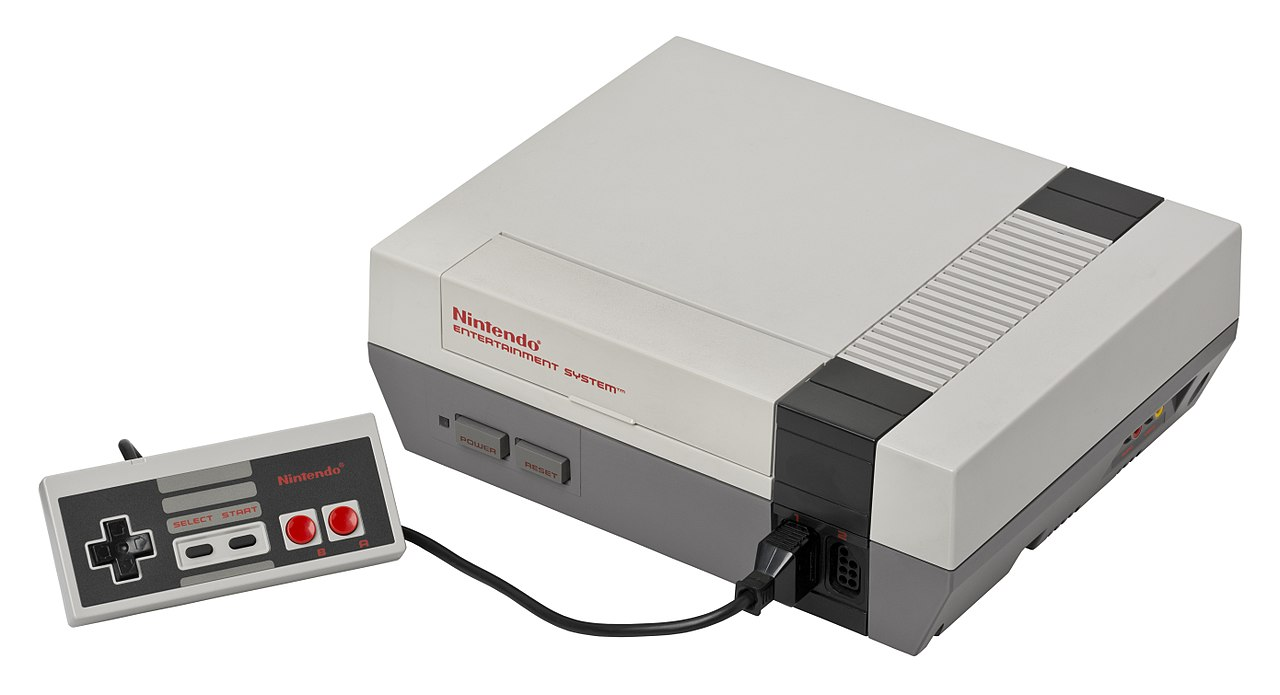
\includegraphics[width=325px, height=175px]{NES_CONSOLE.jpg}\\
\small\textbf{Console Nintendo Entertainment System}
\end{figure}\\
L'emulatore deve, ovviamente, esporre tutte le funzionalità dell'architettura hardware che sta emulando; non serve emulare l'architettura a livello elettrico: per gli scopi del progetto, è sufficiente comprenderne il funzionamento a livello comportamentale, e replicarlo mediante l'ausilio di strumenti tecnologici come il linguaggio C++ o Java, un ambiente di esecuzione, e una macchina host che ospita l'ambiente di esecuzione su cui eseguirà il componente che manifesterà l'emulatore.
\clearpage
Ci teniamo fin da subito a sottolineare che con NES ci si riferisce in genere all'omonima console. Nel nostro caso, poichè il nostro sistema prevede nella fattispecie di sviluppare non solo l'emulatore per la console, ma anche un assemblatore, in grado di poter compilare dei file sorgente scritti dall'utente e produrre così in uscita del codice interpretabile dall'emulatore stesso, allora ci appelleremo al nostro sistema come NES, il cui acronimo tuttavia non sta per \emph{Nintendo Entertainment System}, ma per \emph{NES Emulating System}.

In definitiva, si vuol sviluppare un sistema software, chiamato NES, comprensivo di \emph{emulatore} e \emph{assemblatore}. L'assemblatore consentirà agli utenti del sistema di poter assemblare il proprio programma, scritto ovviamente secondo il modello di programmazione del processore di riferimento montato dalla console, e, consecutivamente, caricare questo programma nell'emulatore consentendo l'esecuzione di quest'ultimo.\\
L'utente deve poter essere in grado di poter interagire con l'assemblatore e assemblare il proprio programma secondo le opzioni messe a disposizione dal sistema stesso; l'utente potrà specificare qualsiasi elemento sintattico appartenente all'ISA della CPU presente nella console: l'assemblatore sarà in grado di interpretare quanto viene specificato dal programma e tradurre il codice e predisporlo per l'esecuzione sull'emulatore.\\
D'altro canto l'utente può decidere di caricare qualsiasi programma assembler sull'emulatore, che sia il programma assemblato con l'assemblatore del sistema, oppure no. L'emulatore non è finalizzato solo all'esecuzione delle linee di codice, ma è destinato anche alla visualizzazione grafica di alcune proprietà interne della macchina emulata durante l'esecuzione del programma, come:
\begin{itemize}
	\item{
		Il comportamento del processore e dei suoi registri interni;
	}
	\item{
		La memoria RAM in qualsiasi range di indirizzi;
	}
	\item{
		Informazioni al contorno;
	}
	\item{
		Il comportamento della PPU e il rendering grafico;
	}
	\item{
		Il comportamento interno della APU.
	}
\end{itemize}
In definitiva, pertanto, l'obiettivo del progetto è chiaramente incentrato sullo sviluppo di un emulatore affidabile, ma non vengono trascurate gli altri aspetti a contorno dell'emulatore, che avranno la loro importanza.
\clearpage
\subsection{Specifiche supplementari}
Tra i requisiti non-funzionali emerge anzitutto la necessità di sviluppare un sistema costituito da componenti \emph{\textbf{riusabili}}; un emulatore mostra davvero la sua utilità qualora il suo meccanismo di emulazione è indipendente dal modo in cui i programmi vengono predisposti per la loro esecuzione. In un progetto si può facilmente comprendere il trascuramento di alcuni di questi requisiti, in quanto la logica dell'emulatore è indubbiamente complessa: se fin da subito, però, si riesce a sviluppare un'architettura costituita da moduli riusabili, ma anche facilmente \emph{\textbf{modificabili}}, allora si potrà fare in modo di adattare l'interfaccia utente all'emulatore sviluppato, senza intaccare la sua logica elaborativa.\\
Oltretutto, non avrebbe senso sviluppare un assemblatore che produca del codice interpretabile solamente dall'emulatore che si sta sviluppando; un approccio lungimirante prevede proprio di rendere \emph{modulare} il sistema e \emph{disaccoppiare} questi due componenti che vanno sotto al nome di assemblatore ed emulatore.

In vista di un approccio agile, e quindi incrementale ed evolutivo, \emph{\textbf{manutenibilità}} e \emph{\textbf{evolvibilità}} sono importanti: entrambi i sottosistemi, essendo complessi, si prestano a essere decomposti in moduli idealmente lascamente accoppiati: bisogna assecondare questa proprietà al fine di ottenere uno sviluppo incentrato sulle parti critiche del sistema, per poter poi \emph{\textbf{estendere}} quanto già sviluppato nelle prime iterazioni.

Si vuole anche rendere il sistema quanto più \emph{\textbf{interattivo}} possibile: data la natura dell'emulatore, il sistema stesso potrebbe risultare poco \emph{\textbf{usabile}}. Le scelte di design dovranno in qualche modo rendere il sistema più user-friendly.
\clearpage
\subsection{Glossario}

In questa sezione presentiamo un documento relativo al mantenimento e all'esposizione di diversi termini che ricorreranno all'interno di tutto il documento; tali termini sono necessari per poter comprendere al meglio, e seguire precisamente, le parti più tecniche relative al dominio applicativo.\\
Come previsto dal processo di sviluppo adottato, ovvero UP, cominceremo a presentare una sfilza di termini adoperati nella prima iterazione, per poi aggiungerne altri man mano che lo sviluppo andrà avanti.

\begin{itemize}
\item{
	\textbf{APU }: Audio Processing Unit, è l'unità elaborativa delegata al processamento del suono, su 8 bit
}
\item{
	\textbf{Background} : Termine con il quale ci si riferisce alla resa grafica degli elementi dello sfondo, contenuti nei secondi 4KB della Pattern Memory
}
\item{
	\textbf{Bus} : Connettore fisico tra tutti i componenti dell'architettura
}
\item{
	\textbf{Cartridge} : Componente fisico contenente il programma nella sua interezza, spesso chiamato anche Cartuccia
}
\item{
	\textbf{CHROM }: Rappresenta la parte di programma contenuta nella Cartridge relativa alle informazioni grafiche
}
\item{
	\textbf{Control Unit }: Unità di controllo della CPU, delegata alla decodifica delle istruzioni, oltre che all'esecuzione del ciclo del processore
}
\item{
	\textbf{CPU }: Unità di processamento, corrispondente al processore fisico 6502, del quale verrà implementato l'ISA
}
\item{
	\textbf{Display }: Componente necessario alla resa grafica; la risoluzione del display sarà quella classica del NES, 240x256
}
\item{
	\textbf{DMA }: Direct Memory Access, componente delegato all'accesso diretto alla memoria, senza passare dal processore ; viene utilizzato per la gestione grafica del foreground
}
\item{
	\textbf{Foreground }: Termine con il quale ci si riferisce alla resa grafica degli elementi più dinamici che si muovono sovrapponendosi allo sfondo, contenuti nei primi 4KB della Pattern Memory
}
\item{
	\textbf{Indirizzamento }: Modalità secondo le quali il processore accede ad i dati. La specifica modalità stabilisce non solo la lunghezza di una istruzione, ma anche dove gli operandi di tale istruzione andranno prelevati
}
\item{
	\textbf{Istruzione }: Incapsula le informazioni binarie relative sia all'Opcode da fare eseguire all'unità operativa, che gli operandi da utilizzare. Tipicamente è a lunghezza variabile e viene estratta dalla Cartridge.
}
\item{
	\textbf{Loopy registers }: Registri ad utilizzo unico della PPU
}
\item{
	\textbf{Joypad }: Componente delegato all'inoltro dei segnali di input
}
\item{
	\textbf{Mapper }: Circuito interno alla cartuccia che realizza il mappaggio tra gli indirizzi virtuali specificati sul bus, e quelli fisici presenti in Cartridge; ne esistono di diversi tipi, ma noi ci riferiremo principalmente al mapper 0.
}
\item{
	\textbf{Mirroring }: Meccanismo di gestione dell'aliasing interno alla memoria
}
\item{
	\textbf{Nametable }: Spazio di memoria dedicato alla memorizzazione di informazioni grafiche. (Tiles e Sprites)
}
\item{
	\textbf{OAM }: Object Attribute Memory, memoria interna alla PPU che contiene una lista di 64 sprites da mostrare a schermo, ognuno dei quali occupa 4 bytes
}
\item{
	\textbf{Opcode }: Codice operativo che stabilisce cosa l'unità operativa dovrà fare
}
\item{
	\textbf{Operative Unit }: Unità operativa del processore, realizza il funzionamento specificato dall'opcode e dall'indirizzamento
}
\item{
	\textbf{Palette }: Tavolozza di colori utilizzati per il rendering di uno specifico tile
}
\item{
	\textbf{Pattern Memory }: Sinonimo di CHROM
}
\item{
	\textbf{Pixel }: unità minima di rappresentazione a schermo; può essere caratterizzato dalla sua posizione e da un colore preso da una palette
}
\item{
	\textbf{PPU }: Picture Processing Unit, unità computazionale delegata alla renderizzazione a schermo
}
\item{
	\textbf{PRGROM }: Parte di memoria della Cartridge contenente le istruzioni del programma da passare alla CPU
}
\item{
	\textbf{Programma }: Insieme di istruzioni interpretabili dal processore 6502
}
\item{
	\textbf{RAM }: Random Access Memory, memoria centrale del sistema, con 2KB di spazio disponibile
}
\item{
	\textbf{Rendering }: Processo tramite il quale avviene la resa grafica a schermo; è un qualcosa di particolarmente elaborato, che fa uso di una logica piuttosto fitta di permutazione di tiles 
}
\item{
	\textbf{Scanline }: Linea "immaginaria" che attraversa orizzontalmente lo schermo, disegnandovi sopra dei pixel, resettandosi ad ogni riga terminata, fino al riempimento dello schermo e oltre. è una astrazione del fascio di fotoni che attraversava lo schermo nei vecchi televisori a tubo catodico
}
\item{
	\textbf{Schermo }: Sinonimo di Display
}
\item{
	\textbf{Scrolling }: Meccanismo grazie al quale la PPU gestisce in maniera fluida gli spostamenti orizzontali, verticali ed eventualmente obliqui. fa affidamento sulla pre-renderizzazione di una parte dello schermo
}
\item{
	\textbf{Shift registers }: Registri a scorrimento usati per trasferire il corretto elemento da renderizzare
}
\item{
	\textbf{Sprite }: Composizione di Tiles, volto alla realizzazione di un elemento del background o del foreground.
}
\item{
	\textbf{Tile }: Elemento di dimensione 8x8 pixel; è il formato standard da considerare nel caso di elemento grafico gestito dal NES
}
\item{
	\textbf{Vertical Blank }: Sezione speciale che corrisponde al rendering esternamente allo spazio visibile dello schermo. Viene utilizzato per resettare alcuni parametri relativi alla prossima elaborazione grafica a schermo
}
\item{
	\textbf{VRAM }: Locazione di memoria atta a contenere informazioni grafiche; si compone di 2 NameTable
}


\end{itemize}

\clearpage

\section{Specifica dei requisiti}
In questa sezione ci riconduciamo ai suggerimenti tratti dal Larman per la stesura dei requisiti funzionali. In particolare, ci concentreremo sulla stesura di artefatti che catturino degli use-case che risultino essere \emph{goal-driven}, ossia incentrandoci sugli obiettivi degli utenti che sfruttano il sistema. Successivamente, sempre nella presente sezione, rivolgeremo la nostra attenzione alle varie features funzionali esposte dal sistema, usufruibili dall'utente, seppure non riconducibili a un obiettivo specifico di quest'ultimo.

\subsection{Attori e Obiettivi}
Attori:
\begin{itemize}
	\item{Utente}
\end{itemize}
Obiettivi utente:
\begin{enumerate}
	\item{
		Esegui programma (Scegliendolo dalla lista o dal file system)
	}
	\item{
		Configura Emulazione (Velocità/Periferica)
	}
	\item{
		Compila il Codice 
	}
	\item{
		Visualizza Stato Architettura 
	}
\end{enumerate}

Descrizione in breve dei casi d’uso:
\begin{itemize}
\item{
	EseguiProgramma: Il programmatore potrà eseguire il programma ed eventualmente visualizzare a schermo l’esecuzione. L’esecuzione potrà essere fatta sia in modalità standard che istruzione per istruzione.
}
\item{
	ConfiguraEmulazione: L’utente prima dell’esecuzione di un programma potrà cliccare su di un pulsante per visualizzare e modificare i parametri di emulazione come la Velocità dell’esecuzione, le periferiche di ingresso e di uscita, la grandezza dello schermo etc. 
}
\item{
	CompilaCodice: Permette di compilare il codice scritto producendo un file macchina comprensibile per l’emulatore.
}
\item{
	VisualizzaStatoArchitettura: Il programmatore potrà cliccare sull’immagine di una specifica componente hardware emulata per verificare il comportamento della stessa durante l’esecuzione di un programma
}
\end{itemize}\clearpage
\subsection{Use-case model}
\subsubsection{EseguiProgramma}
\begin{table}[h]
\begin{tabular}{|l|l|}
\hline
\textbf{Nome del caso d'uso}      & EseguiProgramma                                                                                                                                                                                                        \\ \hline
\textbf{Portata}                  & User-level                                                                                                                                                                                                             \\ \hline
\textbf{Attore primario}          & Utente                                                                                                                                                                                                                 \\ \hline
\textbf{Stakeholders e interessi} & Selezionare il programma ed eseguirlo                                                                                                                                                                                  \\ \hline
\textbf{Pre-condizioni}           & Modalità d'esecuzione scelta                                                                                                                                                                                                                       \\ \hline
\textbf{Post-condizioni}          & Visualizzazione dell'esecuzione del programma                                                                                                                                                                          \\ \hline
\textbf{Scenario principale}      & \begin{tabular}[c]{@{}l@{}}1. Seleziona programma\\ 2. Avvia programma\end{tabular}                                                                                                                                    \\ \hline
\textbf{Estensioni}               & \begin{tabular}[c]{@{}l@{}}1a. L'utente seleziona il programma dalla lista\\ 1b. L'utente seleziona il programma dal file system\\ 2a. L'utente sospende il programma\\ 2b. L'utente arresta il programma\end{tabular} \\ \hline
\end{tabular}
\end{table}
\subsubsection{VisualizzaStatoArchitettura}
\begin{table}[h]
\begin{tabular}{|l|l|}
\hline
\textbf{Nome del caso d'uso}      & VisualizzaStatoArchitettura                                                                                                                                                                                                                                                                             \\ \hline
\textbf{Portata}                  & User-level                                                                                                                                                                                                                                                                                              \\ \hline
\textbf{Attore primario}          & Utente                                                                                                                                                                                                                                                                                                  \\ \hline
\textbf{Stakeholders e interessi} & Verificare l'evoluzione dello stato dell'architettura                                                                                                                                                                                                                                                   \\ \hline
\textbf{Pre-condizioni}           & Il programma è in esecuzione                                                                                                                                                                                                                                                                        \\ \hline
\textbf{Post-condizioni}          & Visualizzazione dello stato dell'architettura                                                                                                                                                                                                                                                           \\ \hline
\textbf{Scenario principale}      & 1. Seleziona componente                                                                                                                                                                                                                                                                                 \\ \hline
\textbf{Estensioni}               & \begin{tabular}[c]{@{}l@{}}1a. Se selezionata la CPU\\ \quad1. Mostra tutti i registri\\ 1b. Se selezionata la memoria\\ \quad 1. Seleziona range\\ \quad 2. Mostra porzione di memoria\\ 1c. Se selezionata la PPU\\ 1d. Se selezionata la APU\end{tabular} \\ \hline
\end{tabular}
\end{table}
\subsection{Feature list}

\subsubsection{Emulazione del Nintendo Entertainment System}
Questo aspetto funzionale è annoverato nella feature list funzionale del sistema; nella fattispecie, consideriamo che un utente voglia usare l'emulatore, ma non è di suo interesse emulare il Nintendo Entertainment System, in quanto questa cosa è interpretabile più come l'effetto piuttosto che la causa che porta l'utente a usare il sistema.\\
In ogni caso, questo è indubbiamente un requisito funzionale, che include in sè tutta una serie di altre feature; prima di discutere di queste altre features, esponiamo in breve l'architettura del NES, che aiuterà a guidare lo sviluppo verso un sistema software la cui parte di logica applicativa sia fedele all'hardware emulato:
\begin{figure}[h]
\hspace*{-1cm}
\centering
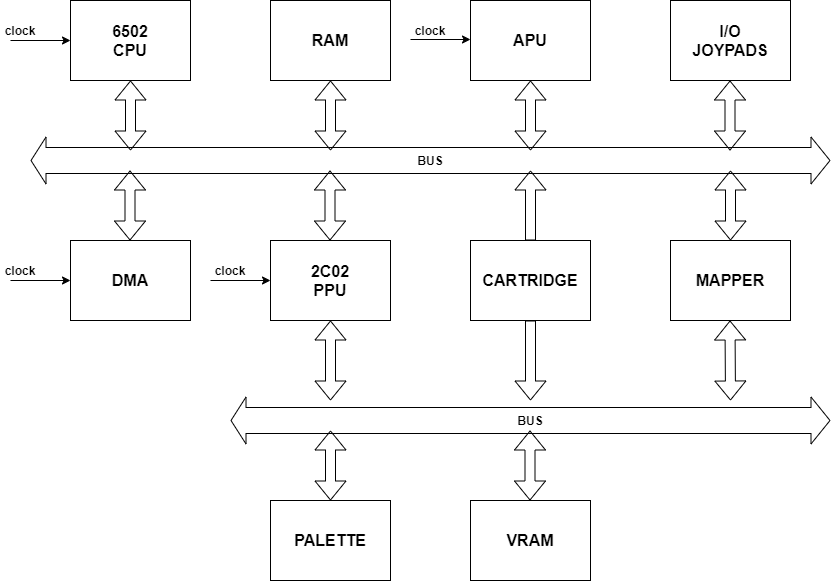
\includegraphics[width=390px, height=270px]{NES_ARCH.png}
\end{figure}\\
Ovviamente l'architettura è complessa, e all'avvio del progetto non è completamente compresa; obbiettivo dello sviluppo iterativo è individuare quali sono i componenti principali, e lavorare sulla loro comprensione, per poi continuare allo sviluppo completo del sistema.\clearpage
\paragraph{Interpretazione del linguaggio assembly per il 6502}
\begin{figure}[h]
\centering
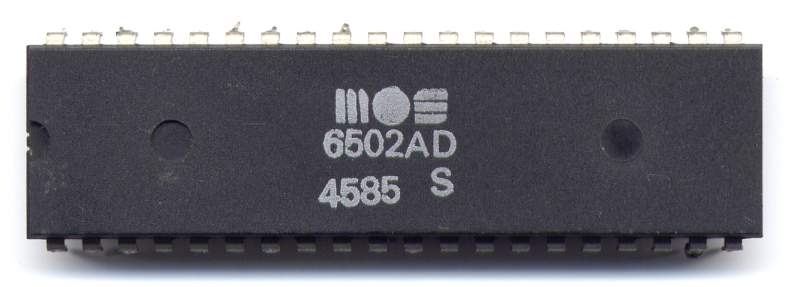
\includegraphics[width=300px, height=110px]{6502.jpg}\\
\small\textbf{Il chip 6502: la CPU che monta il NES}
\end{figure}
L'architettura hardware da emulare possiede una CPU, e il suo comportamento fondamentale è riconducibile a quello di qualsiasi altra CPU in commercio, ossia il percorrimento del \emph{ciclo di Von Neumann}. La CPU possiede due architetture: l'architettura \emph{interna}, che comprende tutti i componenti elementari di cui è costituita la CPU, e l'architettura \emph{esterna}, che lascia invece all'osservatore solo un sottoinsieme dei componenti fondamentali di cui è costituita, oltre che il modo con cui è possibile interagire con la CPU stessa; il modo con cui è possibile interagire si tratta, effettivamente, del \emph{modello di programmazione}: la CPU è una macchina astratta, un interprete, che consente, data un'istruzione, di eseguire tale istruzione e fornire in uscita dei dati. Nella nostra emulazione saremo interessati nel comportamento superficiale della CPU, che d'altronde è in linea con le scelte di progetto che si sono poste sin dall'inizio: non si è interessati a comprendere come i vari segnali si propagano tra il microcontrollore e il datapath della CPU per adempiere a tutte le \emph{microistruzioni} di cui è costituita un'istruzione. L'unica cosa a cui si è interessati è come la CPU risponde, attraverso il suo modello, alle istruzioni fornite alla CPU.
\clearpage
\paragraph{Rendering grafico}
\begin{figure}[h]
\centering
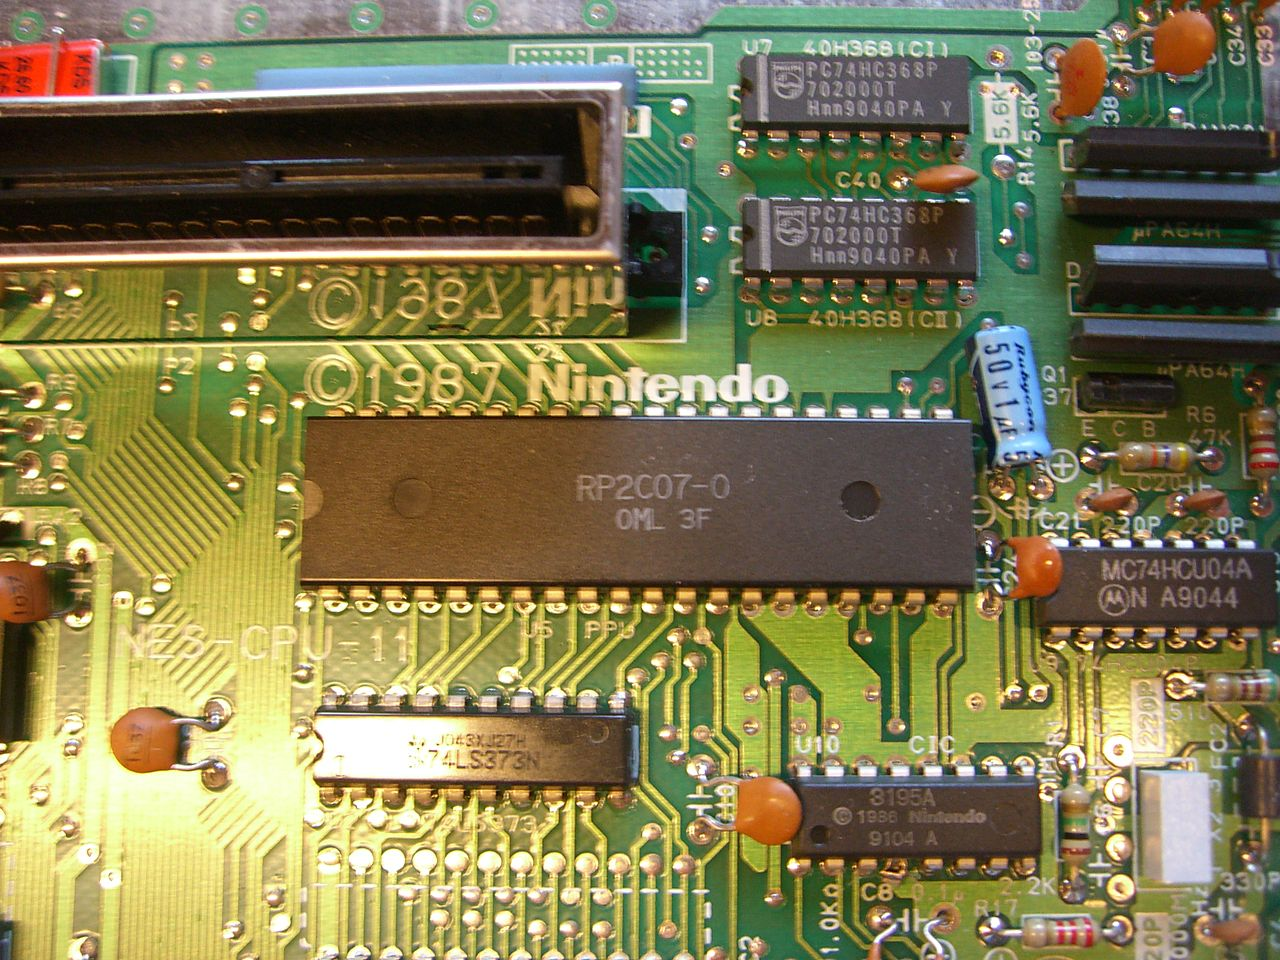
\includegraphics[width=275px, height=206px]{2C02}\\
\small\textbf{Una foto che presenta, tra le altre cose, il chip 2C02: la GPU del NES}
\end{figure}
Insieme all'interpretazione delle istruzioni fornite dalla ROM contenuta nella cartuccia che viene caricata in un NES, non può che esserci una feature fondamentale che consente, di fatto, l'esecuzione dei videogiochi: il rendering grafico. Il rendering grafico è ottenuto mediante la comunicazione della CPU con un componente, denominato PPU. La PPU può essere interpretata come una GPU, ossia in gergo una scheda video, che consente di tradurre le informazioni presenti nella ROM, insieme ad altre memorie, in pixel, ossia degli oggetti che trasportano un'informazione che decodificata rappresenta un colore: il rendering grafico si configura, pertanto, non di meno come il rendering dei pixel attraverso lo schermo.
\paragraph{Lettura periferiche esterne}
Come si nota anche dall'immagine apposta del NES inizialmente, il sistema dovrà prevedere la possibilità di interagire con l'esterno mediante dei `joypad', ossia delle periferiche di input/output che consentano di interagire con il videogioco in esecuzione. Il meccanismo interno della CPU provvederà a leggere dagli opportuni registri, tuttavia bisognerà anche prevedere degli appositi meccanismi per l'interlocuzione delle periferiche con l'emulatore.
\clearpage
\subsubsection{Gestione dei programmi}
\begin{figure}[h]
\centering
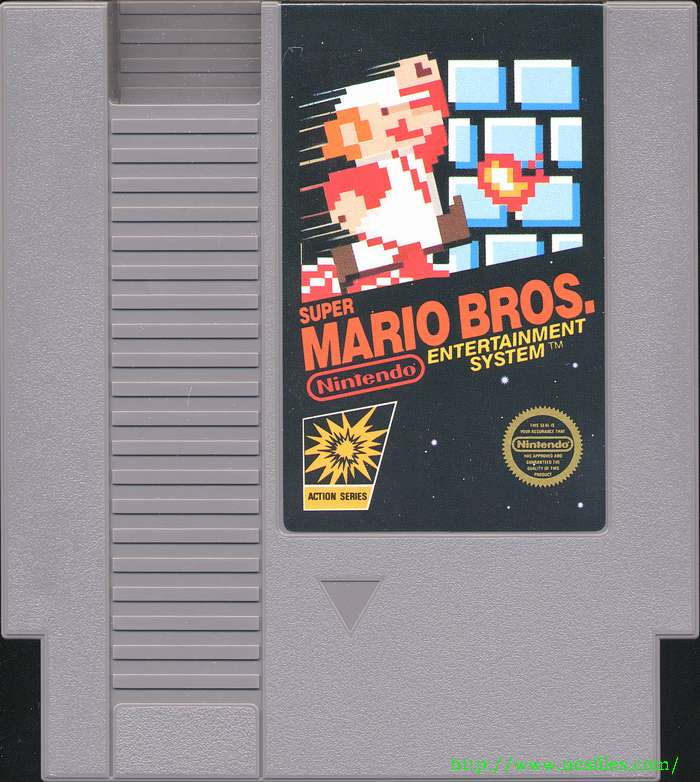
\includegraphics[width=175px, height=195px]{MARIO_ROM.jpg}\\
\small\textbf{Cartuccia per il NES}
\end{figure}
Con il sistema fisico l'utente della console poteva caricare i propri videogiochi mediante le cosiddette cartucce. Nel caso di un'emulazione software dell'architettura hardware, di fatto sarà prevista una gestione delle `cartucce' intese come dati binari memorizzati su piattaforme di immagazzinamento dati persistenti; queste cartucce virtuali vanno sotto al nome generico di programmi, e il sistema prevederà la gestione dei programmi secondo le usuali operazioni CRUD, consentendo tuttavia di poter avere a \emph{diverse} fonti di dati persistenti, il cui accesso dev'essere ovviamente trasparente all'utente.

\subsubsection{Interfaccia grafica}

Prevedendo un sistema in grado di gestire dinamicamente le interazioni con l'utente, abbiamo deciso di annoverare tra le varie feature, anche quella di una interfaccia grafica. Da consegna, l'utente dovrà essere in grado in primo luogo di poter interagire con il sistema, stabilendo alcune configurazioni di base, come la modalità di esecuzione, la grandezza dello schermo, eventuali impostazioni di emulazione e via dicendo.

L'utente dovrà inoltre poter caricare direttamente il programma dal file system, oppure all'interno di una lista mantenuta localmente dal sistema sottoforma di database. è allora chiaro che sarà necessario poter modificare questa lista, inserendo ed eliminando nuovi programmi che si desidera poter avere sempre sottomano.

Dettagliamo brevemente le due possibili modalità di esecuzione:

\begin{itemize}
\item{
\textbf{Utente} : in questa modalità l'utente è solo interessato a potere usufruire dell'emulatore in qualità di Console per videogiochi. ciò significa che l'utente avrà a disposizione unicamente lo schermo sul quale verrà renderizzato il programma; tale programma non sarà necessariamente un videogioco, ma potrebbe essere un qualsiasi programma che preveda un rendering grafico
}
\item{
\textbf{Programmatore} : Questa modalità, decisamente più specializzata, permetterà all'utente non solo di vedere lo schermo con rendering grafico, ma anche di poter visualizzare le informazioni in continua evoluzione di registri del processore e di altre periferiche, nonchè delle svariate memorie.
}
\end{itemize}

Posta una prima interfaccia di configurazione, all'avvio del programma, in base alla modalità scelta, verrà presentata una seconda interfaccia, come specificato dalla modalità poc'anzi illustrata.\\
Ipotizzando di lavorare in modalità "Programmatore", ci aspettiamo che l'utente sia in grado di selezionare di quale periferica analizzare il dettaglio dei registri, e selezionare chiaramente la memoria da mostrare, nonchè il suo range di indirizzamento.

Al contempo è desiderabile poter interagire con dei pulsanti che possano interrompere l'esecuzione, riprenderla, terminarla o addirittura eseguirla \emph{Step by step}; ciò è particolarmente indicato qualora si volesse studiare passo per passo il comportamento di un programma \emph{under test} da parte del programmatore che usufruisce del sistema.\\

\clearpage
\section{Analisi dei requisiti}
L'analisi dei requisiti è stata svolta all'inizio di ogni iterazione. Alcuni requisiti hanno necessitato un approfondimento decisamente più marcato di altri, in parte per l'inesperienza in alcuni campi, in parte per la complessità degli argomenti trattati. In ogni caso, l'analisi dei requisiti è sempre partita da un workshop più o meno lungo svolto tra tutti i membri del team, e ogni volta si è fatto riferimento a un sottoinsieme di funzionalità da sviluppare e requisiti non-funzionali da soddisfare. Consideriamo di seguito tutte le analisi dei requisiti svolte nel corso delle iterazioni.

\subsection{Prima iterazione}
Il primo evidente problema che è stato sollevato è stato quello relativo alla ricerca degli elementi critici del sistema software che dovevano essere sviluppati.\\
Sin da subito è stata posta molta attenzione alla logica dell'emulatore all'interno del nostro NES; in particolare l'elemento più critico che abbiamo considerato è stato proprio la CPU. Prima di ciò, tuttavia, abbiamo già organizzato il sistema NES dal punto di vista statico e predisposto per rispettare i requisiti non funzionali.
\subsubsection{Vista use-case}
Il NES si configura per avere ben pochi casi d'uso che possano essere riconducibili a degli obbiettivi utente. La vista use-case che forniamo in questa istanza è, pertanto, molto povera, ma è essenziale notare che come primo use-case abbiamo considerato \emph{EseguiProgramma}, che consentirà all'utente, almeno per questa prima fase, di poter eseguire un programma molto semplice scritto in assembly secondo l'ISA del 6502.\\
È da notare che, almeno per questa iterazione, non è stato previsto di procedere con l'implementazione, anche solo parziale, di nessuna funzionalità dell'assemblatore, e pertanto non è stato sviluppato alcun use-case diagram.
\clearpage
\begin{figure}[h]
\centering
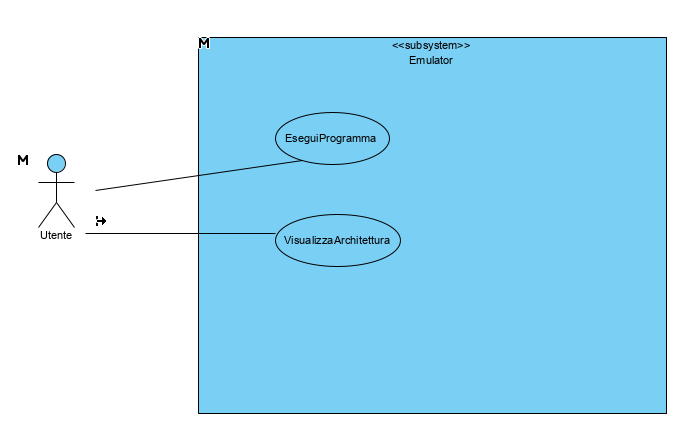
\includegraphics[width=275px, height=171px]{UC_Emulator.png}\\
\small\textbf{UC\_Emulator}
\end{figure}

\subsubsection{Architettura logica}
Abbiamo proceduto anzitutto con la decomposizione modulare dei due sottosistemi di cui il NES è costituito, ossia l'assemblatore e l'emulatore; il che ci ha portato al semplice ma esplicativo primo diagramma che chiarifica i moduli principali del NES:
\begin{figure}[h]
\centering
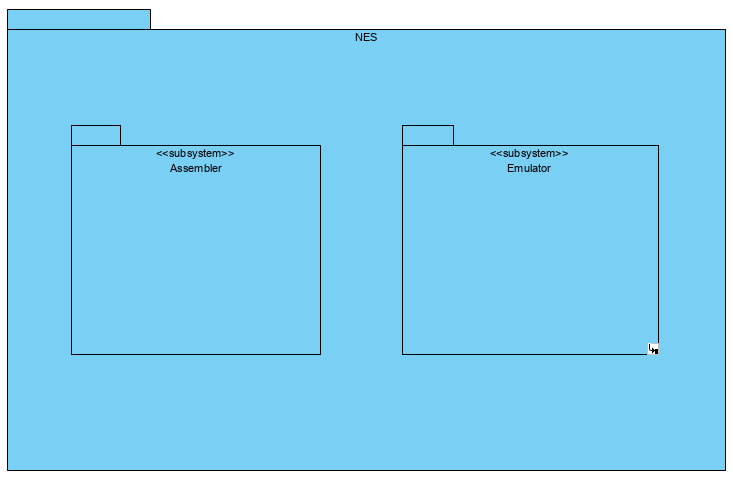
\includegraphics[width=300px, height=191px]{CD_NES_Architecture.png}\\
\small\textbf{CD\_NES\_Architecture}
\end{figure}

\subsubsection{Logica applicativa}
Così come suggerito dall'approccio seguito dal Larman, abbiamo proceduto con l'identificazione, per l'emulatore, delle principali entità costitutive che guideranno il design per la prima iterazione. Prima di ciò, bisogna tuttavia fare una breve parentesi quantomeno sul componente protagonista di questa iterazione, che è proprio la CPU, ovverosia il 6502. 
\paragraph{CPU}
Della CPU, come già accennato, siamo particolarmente interessati al suo comportamento esterno più che alla sua evoluzione dal punto di vista elettrico. Per tal motivo, abbiamo sin da subito ispezionato quello che è il modello di programmazione della CPU montata dal sistema hardware, ossia il 6502. 
\begin{figure}[h]
\centering
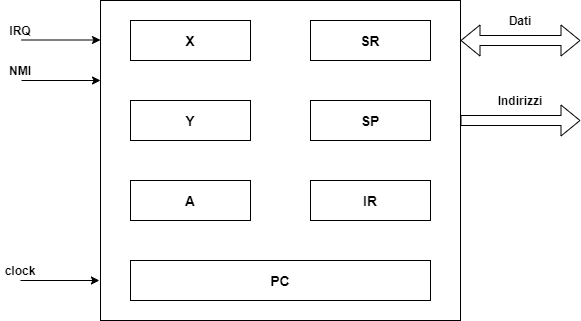
\includegraphics[width=300px, height=166px]{CPU.png}
\small\textbf{Schematizzazione dell'architettura esterna della CPU}
\end{figure}\\
Il modello di programmazione prevede l'interazione con diversi registri:
\begin{itemize}
	\item{
		Il Program Counter è un registro a 16 bit che mantiene la prossima istruzione da indirizzare in memoria;
	}
	\item{
		X e Y sono due registri a 8 bit di utilità per la CPU;	
	}
	\item{
		A è il registro accumulatore;
	}
	\item{
		Lo Status Register mantiene lo stato interno della CPU e viene spesso consultato;
	}
	\item{
		Lo Stack Pointer.
	}
\end{itemize}
I registri sono importanti poichè sono il principale mezzo con cui è possibile comunicare con la CPU. Notiamo, tra le altre cose, anche la presenza di segnali di interruzione (IRQ e NMI, che stanno per Interrupt ReQuest e Non-Maskable Interrupt), il segnale di clock in ingresso alla CPU, e i due bus dati e indirizzi. La CPU possiede un program counter di 16 bit, e può pertanto indirizzare 64KByte di memoria; per il momento supporremo tutta la memoria sia assimilabile a un singolo blocco, che definiamo RAM; vedremo successivamente che in questa architettura hardware gli indirizzi sono spesso sottoposti a un meccanismo specifico, che va sotto al nome di \emph{mirroring}: blocchi di indirizzi non hanno valenza fisica, ma sono solamente `virtuali', il loro contenuto specchia quello degli indirizzi fisicamente presenti. 

Oltre queste considerazioni, il modello di programmazione della CPU può essere pienamente descritto facendo un breve riferimento ai codici operativi e alle modalità di indirizzamento. Come è noto, le istruzioni di una CPU non sono tutte uguali: alcune CPU hanno istruzioni a lunghezza fissa, altre hanno istruzioni a lunghezza variabile, altre hanno istruzioni con quanti fissi ma numero di quanti differenti. Per ciò che riguarda il 6502, le istruzioni sono costituite da diversi quanti da 8 bit ciascuno; dunque si ha una istruzione che ha una lunghezza minima di 1 byte fino ad arrivare a diversi byte di lunghezza. I diversi byte di lunghezza sono determinati sia dalla particolare istruzione, che specifica un numero minimo di operandi, e sia dal modo di indirizzamento.
\clearpage
Combinando codici operativi e modi di indirizzamento, si ottengono diverse permutazioni; il 6502 implementa molti modi di indirizzamento, disponibili per molti codici operativi, configurandosi come un'architettura quasi-ortogonale. In ogni caso, il numero totale di possibilità sono 256; molte delle possibilità, tuttavia, costituiscono dei codici operativi illeciti, che mostrerebbero, su un'architettura reale, un comportamento imprevedibile.
\begin{figure}[h]
\hspace*{-1cm}
\centering
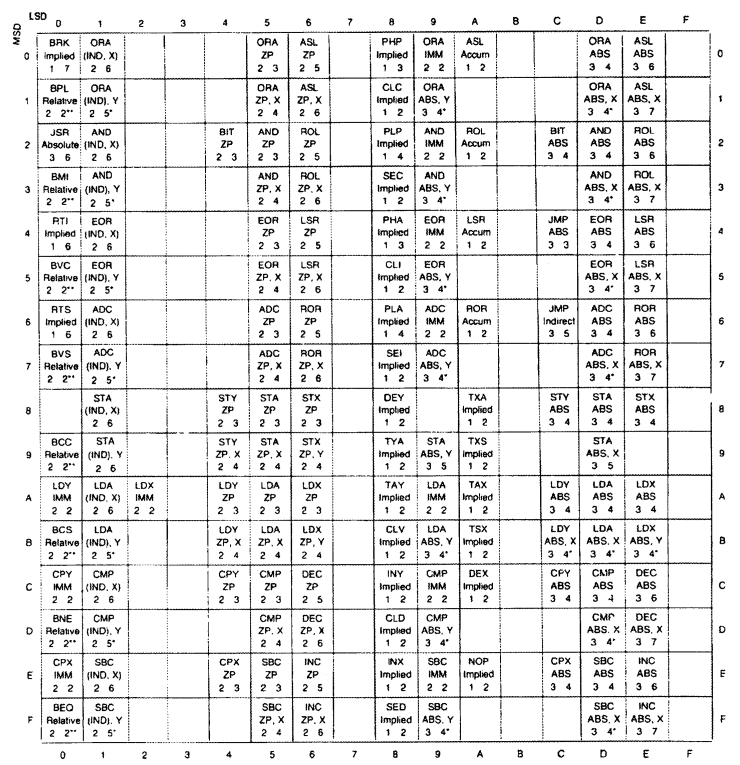
\includegraphics[width=400px, height=400px]{6502_INSTRUCTION_SET.png}
\small\textbf{ISA del 6502}
\end{figure}
\clearpage
\paragraph{System Domain Model} Siamo adesso pronti a presentare il System Domain Model, catturato secondo la notazione UML facendo uso dei costrutti tipici di un class diagram:
\begin{figure}[h]
\centering
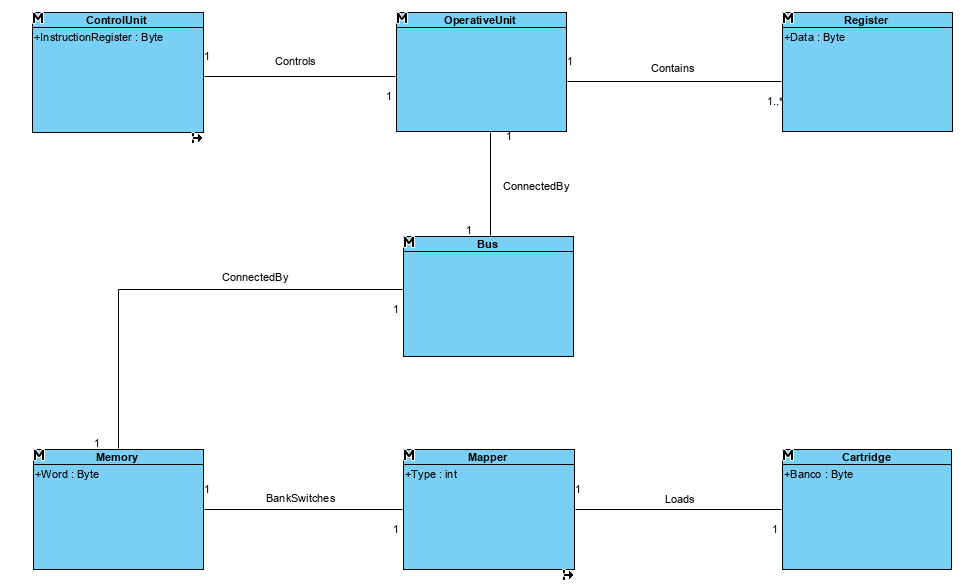
\includegraphics[width=375px, height=225px]{CD_DomainModel.png}\\
\small\textbf{CD\_DomainModel}
\end{figure}\\
Il diagramma cattura le prime entità di dominio; ricordiamo in questa istanza che le classi che vengono raffigurate non fanno riferimento ad alcuna classe software, rappresentano dei concetti, con una loro \emph{intensione}, ossia un loro significato intrinseco, e una loro \emph{estensione}, ossia in che modo esse si relazionano con le altre classi. Di seguito, quindi, una breve descrizione delle classi concettuali catturate:
\begin{itemize}
	\item{
		\emph{ControlUnit}\\
		La classe \emph{ControlUnit} rappresenta un concetto molto chiaro e immediato: un'entità che ordina e controlla l'intera logica applicativa, che in base alle istruzioni di cui
		dispone, è in grado, tramite l'interazione con le altre classi, di comandare l'esecuzione di un programma;
	}
	\item{
		\emph{OperativeUnit}\\
		Questa classe è direttamente collegata alla \emph{ControlUnit}; di fatto, una CPU può essere schematizzata in unità di controllo e unità operativa; tuttavia l'unità operativa
		può essere ritenuta come un concetto a parte, poichè non controlla niente, bensì evolve il proprio stato sulla base degli ordini forniti dall'unità di controllo.
	}
	\item{
		\emph{Register}\\
		I registri sono quelli che sono stati esposti poc'anzi, e sono quelli che, per l'appunto, rappresentano lo stato dell'unità operativa; essi evolvono sulla base delle operazioni svolte
		dall'unità operativa;
	}
	\item{
		\emph{Bus}\\
		Elemento centrale dell'architettura, al bus è demandato il direzionamento della comunicazione verso gli altri elementi dell'architettura;
	}
	\item{
		\emph{Memory}\\
		La memoria incapsula uno spazio riservato ad alcune informazioni che vengono scambiate dalla CPU verso questa entità. Di fatto, non è possibile considerare questa
		entità a un livello di vicinanza come quello dei registri, in quanto la memoria non rappresenta lo stato interno dell'unità operativa, bensì una sorgente dati che sopperisce
		alla limitatezza dei registri;
	}
	\item{
		\emph{Mapper}\\
		Il mapper è un'entità strettamente legata alla cartuccia, ma concettualmente diversa: essa si configura come una sorta di controllore, direziona le richieste di comunicazione
		della CPU verso la cartuccia filtrandole e gestendole opportunamente;
	}
	\item{
		\emph{Cartridge}\\
		Ultimo concetto esposto da questo diagramma, la cartuccia rappresenta l'insieme di dati che verrà continuamente interrogato dalla CPU nel contesto di esecuzione di un 
		programma.
	}
\end{itemize}
\subsubsection{Cattura degli eventi esterni}
Uno dei primi problemi a cui ci si è interessati è stato la cattura degli eventi esterni inoltrati dall'utente. A tale scopo, è stato introdotto un diagramma che ha arricchito il \emph{System Domain Model} precedentemente sviluppato, che ha introdotto delle nuove classi. Il diagramma è mostrato nella seguente pagina.\\
\begin{figure}[t]
\hspace*{-1cm}
\centering
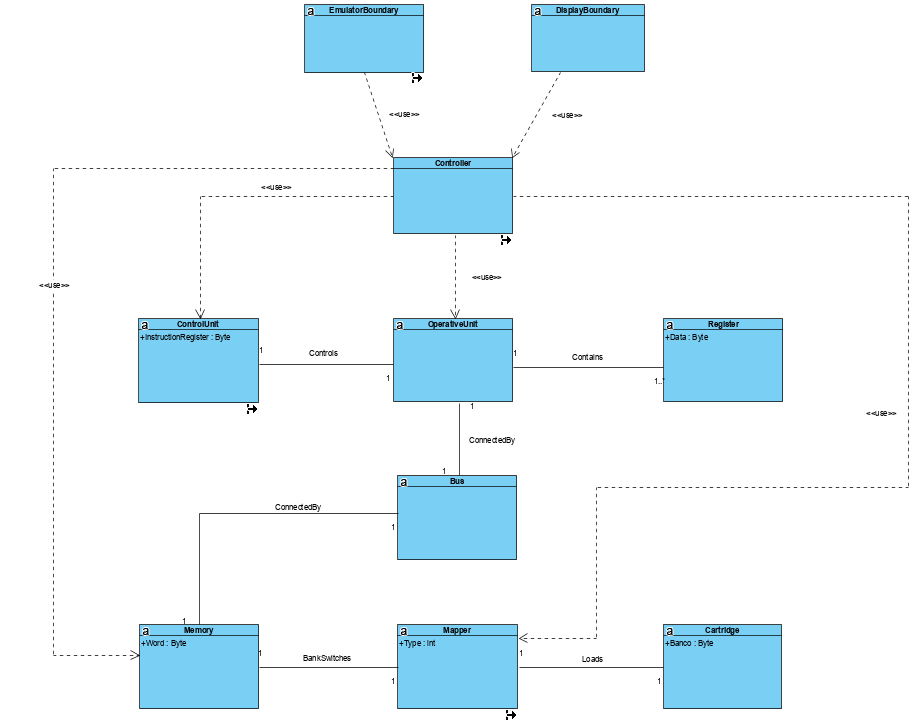
\includegraphics[width=420px, height=330px]{CD_Domain_Boundary_Controller.png}\\
\small\textbf{CD\_Domain\_Boundary\_Controller}
\end{figure}
Questo diagramma è stato il frutto dell'introduzione di due classi, che incapsulano concetti propri di una futura interfaccia grafica; la classe \emph{EmulatorBoundary} sarà responsabile di avviare la comunicazione con l'utente, consentendo a quest'ultimo di interloquire con l'emulatore, mentre la classe \emph{DisplayBoundary} fornirà all'utente informazioni grafiche, che si configurano specialmente per le varie possibilità che verranno aperte all'utente in quanto a visualizzazione a schermo. A questo punto, mediante l'applicazione del pattern GRASP Controller, abbiamo introdotto una classe \emph{Controller} che si occuperà di raccogliere le richieste inoltrate dalle classi di interfacciamento con l'utente con la logica dell'applicazione.\clearpage
A partire da questo diagramma si può già aprire il primo diagramma sulla dinamica che guiderà la fase di design; questo diagramma mostra nella sua essenza il flusso di controllo, con le classi mostrate in questo diagramma, che c'è nel contesto del caso d'uso \emph{EseguiProgramma}:
\begin{figure}[h]
\hspace*{-4.1cm}
\centering
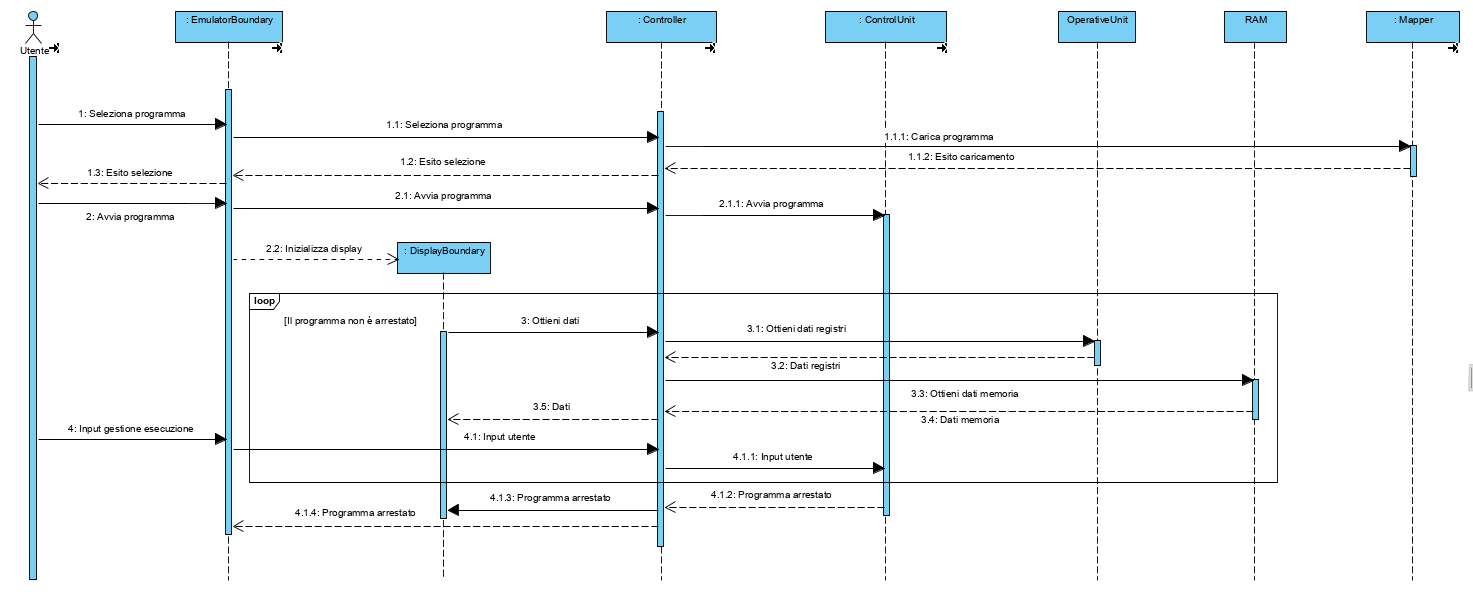
\includegraphics[width=600px, height=241px]{SQD_EseguiProgramma.png}\\
\small\textbf{SQD\_EseguiProgramma}
\end{figure}\\
La lettura è molto chiara; essenzialmente l'utente interagisce con la classe \emph{EmulatorBoundary} per selezionare dapprima il programma (che innescherà un caricamento del programma tramite la classe \emph{Mapper}), e a cui segue poi l'avvio del programma, con inizializzazione del display, recupero dello stato della macchina in esecuzione, e la possibilità di poter gestire gli input degli utenti (anche tramite i cosiddetti Joypad).
\clearpage
\subsection{Seconda iterazione}
\subsubsection{Premessa}
Nella seconda iterazione ci sono stati molti cambiamenti, sia nella stesura dei diagrammi, più coscienziosa e precisa in quanto il gruppo ha raggiunto una maggiore maturità e dimestichezza con gli strumenti a disposizione, sia perchè come team siamo riusciti a comunicare meglio le nostre scelte, discutere sui problemi riscontrati nella precedente iterazione, e quindi apportare delle modifiche importanti. Fortunatamente le scelte di progetto fatte nella prima iterazione hanno favorito le modifiche, poichè la struttura scelta ha facilitato il cambiamento dei requisiti, e l'aggiunta di nuove features. \\
Non sarà quindi raro ritrovare diagrammi già esposti nella prima iterazione, ma ciò è stato interpretato dal gruppo come una cosa giusta, in quanto il processo adottato prevede proprio l'evoluzione dei requisiti, e quindi anche una revisione di quanto già fatto.

\subsubsection{Logica applicativa}
Dal punto di vista architetturale, l'organizzazione a livelli è rimasta del tutto immutata. Ciò che è mutato in maniera decisa, tuttavia, è stato il \emph{System Domain Model}; a causa di una mal interpretazione di elementi del sistema che non erano invero interesse della prima iterazione, la loro modellazione è stata imprecisa in alcuni punti, totalmente sbagliata in altri. Ripresentiamo, quindi, il \emph{Domain Model}, sotto la luce di una revisione concettuale del dominio, nella successiva pagina.\\
Quel che si nota in prima battuta è un infoltimento del diagramma, ciò soprattutto in vista dello sviluppo dei nuovi concetti (ricordiamo, infatti, che lo use-case EseguiProgramma è complesso e ingloba in sè molte altre feature, che bisogna modellare e implementare). Ma si possono notare anche alcune correzioni, come l'eliminazione dell'associazione tra \emph{Memory} e \emph{Mapper}, e il collegamento diretto del \emph{Bus} verso il \emph{Cartridge}; quest'ultimo è solo un esempio di come un'analisi più approfondita verso la materia d'interesse per la corrente iterazione ha portato a un miglioramento del modello.
\clearpage
\begin{figure}[h]
\hspace*{-1.7cm}
\centering
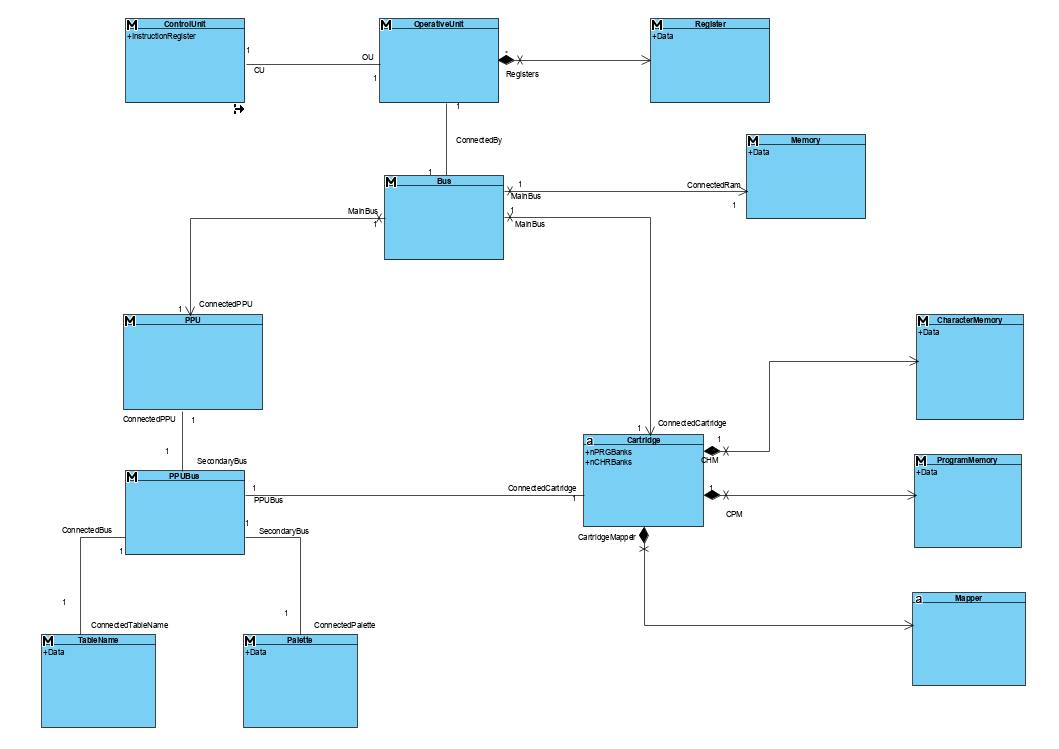
\includegraphics[width=450px, height=320px]{CD_DomainModel_1.png}\\
\small\textbf{CD\_DomainModel}
\end{figure}
Tra le altre cose, abbiamo anche provveduto ad aggiungere alcune classi che saranno utili per il caricamento effettivo della ROM all'interno dell'architettura. Abbiamo:
\begin{itemize}
	\item{
		\emph{PPU}, che concettualmente individua il componente che si farà garante del rendering grafico della ROM che viene caricata in memoria;
	}
	\item{
		\emph{PPUBus}, che sarebbe il componente che redireziona le richieste di lettura e scrittura da parte della PPU verso gli altri componenti;
	}
	\item{
		\emph{TableName}, che rappresenta, di fatto, la VRAM della PPU e mantiene pertanto le informazioni che saranno oggetto effettivo del rendering grafico;
	}
	\item{
		\emph{Palette}, un'altra memoria che incapsula le informazioni a riguardo della Palette dei colori da renderizzare;
	}
	\item{
		\emph{CharacterMemory}, una parte della memoria mantenuta dalla \emph{Cartridge}, che mantiene le informazioni grafiche della ROM;
	}
	\item{
		\emph{ProgramMemory}, simile alla \emph{CharacterMemory}, quest'ultima mantiene le informazioni a riguardo delle istruzioni mantenute dalla ROM da far eseguire alla CPU.
	}
\end{itemize}
Ovviamente queste modifiche si sono riversate anche nel diagramma di dominio arricchito delle classi boundary e della classe controller.
\paragraph{Mapper} Dato che in questa presente iterazione, per quanto concerne la logica applicativa, sarà necessario approfondire il meccanismo di caricamento della cartuccia all'interno dell'emulatore, è bene fare una parentesi sul Mapper.
\begin{figure}[h]
\centering
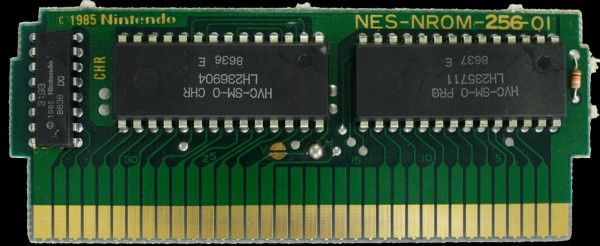
\includegraphics[width=225px, height = 93px]{ROM.jpg}\\
\small\textbf{Una cartuccia fisica, dove sono ben visibili la Program ROM, la Character ROM e il Mapper a lato sulla sinistra}
\end{figure}\\
Quando la CPU desidera comunicare con la cartuccia, e quindi leggere dalla sua \emph{Program ROM}, ciò che avviene è diverso dal fare riferimento al range di indirizzi del mapper. Poichè la CPU riserva per l'indirizzamento verso la cartuccia solamente 32KByte, le cartucce dei videogiochi caricati nel NES sarebbero estremamente semplici, tanto semplici che avrebbero reso il NES obsoleto nel giro di pochissimo tempo. In realtà i progettisti del NES, sotto questo punto di vista molto previdenti, hanno previsto un circuito ausiliario, definito \emph{Mapper}, che ogni cartuccia monta. Il mapper si configura come un vero e proprio intermediario, traducendo gli indirizzi emessi dalla CPU con il corretto contenuto della cartuccia (trattasi propriamente di \emph{bank switching}, ossia scambio di banchi durante l'esecuzione del videogioco).\\
Il nostro emulatore dovrà necessariamente emulare questo meccanismo, e consentire, pertanto, alla CPU di interloquire con questo mapper, prima che, ovviamente, possa trarre il contenuto dalla cartuccia (un meccanismo di traduzione degli indirizzi che rassomiglia quello di una MMU).\\
Un'ultima cosa importante da dire a riguardo dei Mapper riguarda il fatto che ogni ROM monta, concettualmente, un mapper diverso. Ne esistono molti; nel nostro caso, faremo particolare riferimento al mapper più semplice, che nella comunità è appellato come `Mapper 0'.

\subsubsection{Interfaccia grafica}
Durante questa iterazione ci siamo dedicati anche alla progettazione più concreta relativa all'interfacciamento utente.\\
In base a quanto stabilito in origine, l'iterfaccia si sarebbe dovuta comporre di due fondamentali "porti" di interfacciamento, ovvero delle vere e proprie entità di confine, chiamate rispettivamente \textbf{Emulator Boundary} e \textbf{Display Boundary}.

Nonostante tali entità non ritrovino un corrispettivo reale nel nostro modello, esse sono fondamentali per stabilire i confini del sistema nei confronti dell'attore, ovvero l'utente, che vi interagisce.\\
Per quanto detto l'Emulator Boundary dovrà necessariamente prevedere il primo interfacciamento dell'utente, e per quanto visto dall'activity Diagram presentato in precedenza, esso sarà anche responsabile per la creazione di diversi \emph{flussi concorrenti}.

Dall'activity Diagram possiamo infatti notare che l'Emulator Boundary sarà responsabile per la selezione del programma, sia esso da DB o da File System, oltre che dell'esecuzione dello stesso. Sarà poi il Display Boundary a doversi occupare dell'interfacciamento con lo stato, e dell'aggiornamento della \emph{vista}, che sarà mutevole in base alle interazioni con l'utente.

I flussi concorrenti previsti, e visibili nel diagramma, possiamo cominciare a descriverli brevemente:

\begin{itemize}
	\item{
		\emph{Flusso di avvio logica} : il flusso concorrente che si occuperà di avviare il motore sottostante per l'emulazione
	}
	\item{
		\emph{Flusso di visualizzazione dello stato}: il flusso delegato al prelievo dello stato del motore sottostante, e all'aggiornamento conseguente della vista
	}
	\item{
		\emph{Flusso di gestione input}: il flusso responsabile della cattura degli input utente per poter sospendere, riprendere,terminare l'esecuzione
	}
\end{itemize}

Fatta questa prima premessa, si è anche specificato come lo stesso Display Boundary possa essere in grado di creare altri flussi concorrenti per la visualizzazione dei singoli componenti. 
Naturalmente la modellazione di flussi concorrenti si rende necessaria, e dunque abbiamo scelto di applicare nuovamente un activity diagram, collegato alla visualizzazione dello stato dell'architettura, per esplicitare il funzionamento descritto.

\begin{figure}[h]
\centering
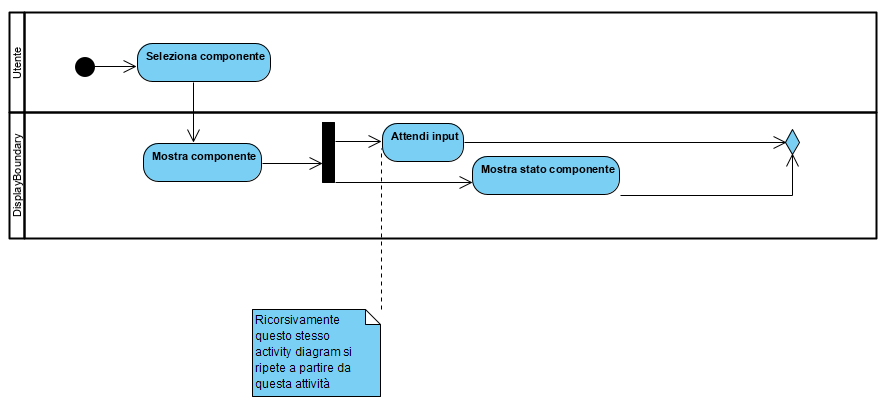
\includegraphics[width=275px, height = 133px]{AD_VisualizzaStatoArchitettura.png}
\end{figure}
\small\textbf{Activity Diagram per la visualizzazione dello stato dell'architettura}\\

\subsubsection{Interfacciamento con File System e Database}
Nella presente iterazione approfondiremo i meccanismi di interfacciamento con le fonti di dati persistenti. Ci saranno due fonti di dati persistenti, che sono, come già enunciato nel titolo, File System e Database; l'obbiettivo è quello di arrivare al termine dell'iterazione disponendo di un meccanismo per caricare i dati di una ROM dal File System o dal Database, secondo il formato binario. In questo caso, è bene fare una specificazione: il contenuto delle ROM è ovviamente binario, in quanto le istruzioni sono codificate in quanti da 2 byte ciascuno. Quindi, quando da un file, o comunque da una tabella all'interno del database, vengono letti due byte, tali due byte sono parte di un'istruzione, o tutta l'istruzione.\\
Nel caso di un file nativamente binario, e quindi in formato \emph{ines} o \emph{nes}, il problema non sussiste: è sufficiente sviluppare una lettura da file byte per byte, e creare opportune strutture per memorizzare i byte che vengono tratti dal file binario. Nel caso di file di testo che contengono il contenuto binario codificato in esadecimale, c'è da fare una puntualizzazione.\\
Supponiamo che il file di testo abbia una forma del tipo:
\begin{lstlisting}
4E45531A010100000000000000000000A9008D00208D0
\end{lstlisting}
bisogna considerare che seppure i singoli caratteri vanno intesi come il risultato di una conversione da stringa binaria a esadecimale, la lettura da un file di testo non è così banale. Se ci aspettiamo che \texttt{A} è il risultato della codifica in esadecimale della stringa binaria \texttt{1010}, nel caso di lettura da file di testo in realtà \texttt{A} è la codifica in formato ASCII della lettera A, che è su 8 bit, e corrisponde a \texttt{01000001}.\\
Prevedere una conversione di questo formato per la lettura da file non è relegato solamente a casi eccezionali di questo tipo. Prevediamo che la memorizzazione su database venga svolta proprio convertendo in esadecimale le informazioni binarie: se non prevediamo un meccanismo, una volta recuperati da database i dati in codifica esadecimale, per riconvertire le informazioni, allora non riusciremmo a gestire le eventuali codifiche dei file, la memorizzazione su database, la gestione interna dei programmi, ecc.

\clearpage
\subsection{Terza iterazione}
\subsubsection{Premessa}
Arrivati alla terza iterazione, il gruppo ha raggiunto molta più maturità. I diagrammi svolti arrivano a un livello di qualità molto più alto, la comunicazione è agevole, e accordarsi sulle scelte diventa più facile in quanto tutti sono allineati sulle giuste scelte da svolgere. I workshop sono più brevi e concisi, e la suddivisione dei compiti più organizzata.\\
Una delle più grandi difficoltà incontrate in questa iterazione ha riguardato il testing di integrazione di tutte le features implementate; il testing è proceduto consultando dei log presenti online che mostravano la corretta esecuzione di alcune ROM, oltre che l'ausilio di alcuni test automatizzati per il 6502 presenti in rete.\\
Un'altra importante sfida è stata la comprensione, modellazione e implementazione della PPU; dispositivo molto complesso, ha necessitato di molti giorni perchè venisse digerito e compreso da tutti. Da queste parole si comprende perchè per la PPU è stata riservata una sezione così ampia come quella che verrà: la comunicazione tra i membri del gruppo è stata di fondamentale importanza. 

\subsubsection{Gestione delle interrupt}
Come ogni CPU che si rispetti, anche il 6502 consente di gestire le richieste di interruzioni provenienti da altri dispositivi; la routine seguita è molto semplice: viene salvato lo stato del sistema nello stack (status register e program counter), per poi interpellare un indirizzo a cui è presente l'istruzione a cui saltare per eseguire la ISR.

\subsubsection{Gestione della tempificazione}
Introducendo in questa iterazione nuovi sistemi che necessitano di essere tempificati (in gergo, `clockati'), si è rivelato indispensabile ricorrere ad analizzare quali sono i dispositivi che necessitano del clock per poter eseguire, anche se ovviamente ciò si ridurrà a `simulare' il clockaggio (in linea con l'interesse di emulare a livello comportamentale l'architettura).

\subsubsection{Comunicazione con l'I/O}
Come è già stato anticipato nelle precedenti sezioni, la CPU 6502 comunica con uno spettro di dispositivi tra loro anche molto diversi. Oltre che la RAM, esistono dispositivi come la Cartridge, la PPU, i Joypad, il DMA, ecc. Tutte le comunicazioni che non avvengono con la RAM e con la Cartridge sono state da noi astratte come `comunicazione I/O', per gestire quindi un vero e proprio sottosistema di input/output, verso cui redirezionare le richieste della CPU. 

\subsubsection{PPU}
La Picture Processing Unit (PPU) è vista dalla CPU montata dal NES come un dispositivo I/O; infatti, la comunicazione con questa unità avviene mediante dei registri (trattasi di \emph{memory-mapped I/O}). La PPU può però essere pienamente classificata come un'unità di elaborazione molto complessa, probabilmente, dal punto di vista implementativo, ancor più della CPU.\\
Essa è ovviamente una macchina sequenziale, che evolve in diversi stati; il suo obbiettivo è quello di \emph{renderizzare}, ossia \emph{disegnare} a schermo, i vari pixel che derivano dalle memorie attaccate alla PPU, ma anche interne alla Cartridge. Detto ciò, analizziamo il sottosistema d'interesse:
\begin{figure}[h]
\hspace*{-2cm}
\centering
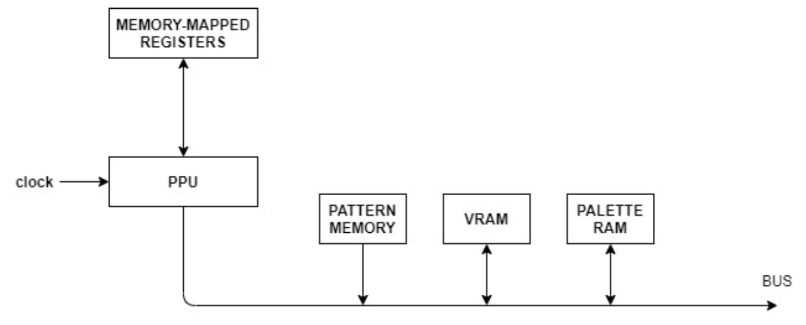
\includegraphics[width=400px, height=156px]{PPUARCH.jpg}
\end{figure}\\
Come si vede, a connettere la PPU è un BUS, che consente il colloquio della PPU con le memorie che sono ad essa fisicamente (e logicamente) accoppiate. In particolare abbiamo:
\begin{itemize}
	\item{
		Pattern Memory\\
		La pattern memory è essenzialmente dove sono memorizzati i disegni sviluppati dai programmatori e che vengono visualizzati a video. È una ROM da 8KByte;
	}
	\item{
		VRAM\\
		La VRAM, o anche Name Table Memory, è la memoria che la PPU utilizza per renderizzare i frame. È molto importante, ed è ovviamente la più complicata, in quanto deve in
		qualche modo mettere insieme le informazioni della ROM con la \emph{palette RAM}. La VRAM occupa 2 KByte di memoria;
	}
	\item{
		Palette RAM\\
		La Palette RAM è una piccola memoria da 64 Byte che consente la memorizzazione dei colori utilizzati per renderizzare i pixel. È scritta dal programma quand'esso andrà
		in esecuzione, ed è gestita in maniera peculiare, così come vedremo successivamente.
	}
\end{itemize}
Per dare una breve panoramica sin da subito su come il meccanismo funziona, prendiamo in esame la VRAM.\\
La VRAM contiene le informazioni per poter individuare un singolo \emph{tile}, o, a un livello di granatura più fine, il singolo \emph{pixel}. La VRAM è costituita da due array, ognuno da $32\times32$ byte, di cui però solo $32\times30$ sono destinati al rendering finale del frame, mentre il rimanente spazio è destinato a determinare gli \emph{attributi} dei tile da renderizzare. Ogni byte fa riferimento a un particolare ID da trarre nella \emph{pattern memory}. Combinando le informazioni tra il tile (o meglio, il pixel) indirizzato dalla VRAM, e l'informazione relativa alla palette, recuperata dalla \emph{attribute memory} (le due righe del singolo array della VRAM non rappresentative di pixel), è possibile \emph{renderizzare un singolo pixel}.

Concettualmente, quindi, disponendo del pixel e dell'attributo relativo al pixel, possiamo disegnare tale pixel.\\
Abbiamo quindi da esplorare quattro cose:
\begin{enumerate}
	\item{
		La gestione della pattern memory;
	}
	\item{
		La gestione della palette memory;
	}
	\item{
		Lo scrolling;
	}
	\item{
		Il rendering.
	}
\end{enumerate}
tenendo a mente che, sotteso a ogni fase, è presente la comunicazione con la CPU attraverso i memory-mapped registers.
\clearpage
\paragraph{Gestione della pattern memory} La pattern memory risiede sulla cartridge, ed è organizzata in due blocchi da $4KByte$ ciascuno:
\begin{figure}[h]
\centering
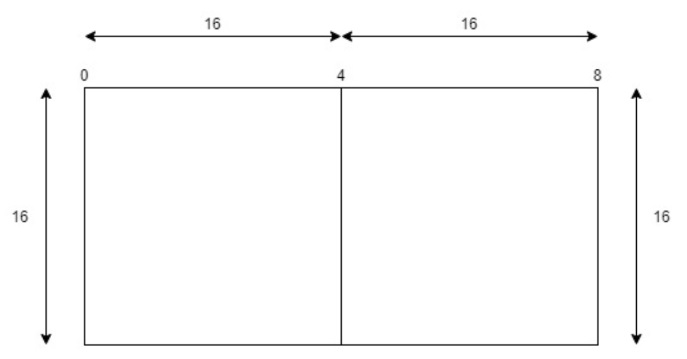
\includegraphics[width=350px, height=175px]{PATTERNMEM.jpg}
\end{figure}\\
Ogni blocco può essere considerato come costituito da $16\times16$ tiles, dove ogni tile non è altro che un agglomerato di pixel. Ogni pixel mantiene un'informazione da 2 bit, e pertanto, poichè ogni tile è $8\times8$ pixel, allora per ogni tile sono necessari 128bit, ossia \emph{16 byte}. Questi 16 byte sono memorizzati tramite i due \emph{bit plane} in cui è decomponibile un tile. Dunque, visualizzando questa tecnica, abbiamo:
\begin{figure}[h]
\centering
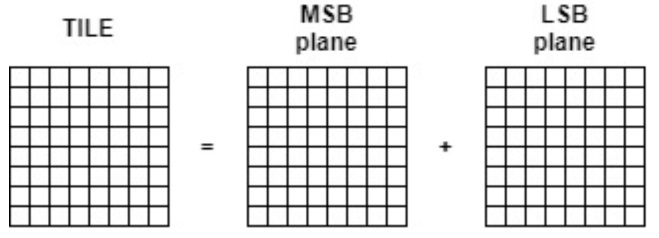
\includegraphics[width=322px, height=116px]{TILE_STORING.jpg}
\end{figure}\\
Il valore contenuto dal pixel ci sarà utile per determinare il suo colore.
\clearpage
\paragraph{Gestione della palette memory}
La palette memory è gestita facendo uso di una piccola porzione dello spazio di indirizzamento della PPU, ossia da $\$3F00$ a $\$3FFF$, con mirroring a partire da $\$3F20$.\\
La palette memory è così organizzata:
\begin{figure}[h]
\centering
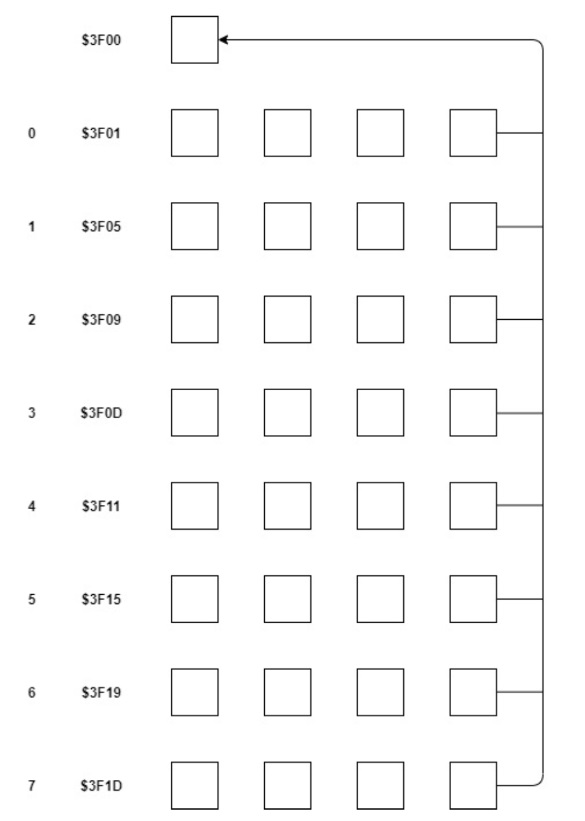
\includegraphics[width=275px, height=400px]{PALETTE_STORING.jpg}
\end{figure}\\
Con quei numeri a fianco degli indirizzi, si indica l'indice della i-esima palette. Nel contesto della palette, oltre all'indice va specificato anche l'offset, per campionare lo specifico colore della specifica palette. La formula è:
\[
	(\textrm{PaletteID}\cdot 4)+\textrm{offset}=\textrm{colore}
\]
Da notare che per ogni palette c'è un mirroring al colore mantenuto da $\$3F00$, che è il background.

Dunque, concettualmente, il programma \emph{carica} la palette memory, \emph{carica} la pattern memory, e quando la \emph{VRAM} riesce a indirizzare un pixel dalla pattern memory, combinando questa informazione con ciò che è contenuto nell'attributo relativo al pixel, si può ottenere il colore corretto per il pixel da disegnare.
\paragraph{Gestione dello scrolling} Poniamo qui particolare enfasi sulla configurazione grafica della VRAM:
\begin{figure}[h]
\centering
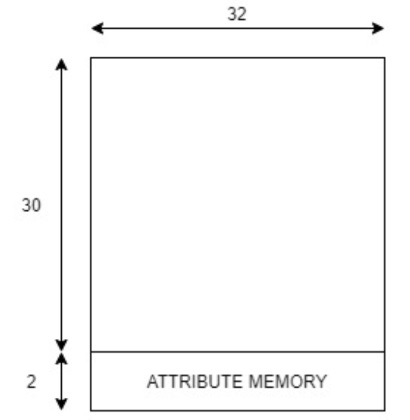
\includegraphics[width=200px, height=215px]{NAMETABLE.jpg}\\
\small\textbf{Nametable}
\end{figure}\\
Spesso i programmi, nel passare da un frame a un altro, cambiano solo lievemente lo scenario, dando l'impressione di star srotolando una bobina (in verticale o in orizzontale). Ciò apre le porte a un meccanism ocomplesso ma fondante della logica di rendering: lo scrolling.
\clearpage
Consideriamo lo scrolling orizzontale:
\begin{figure}[h]
\centering
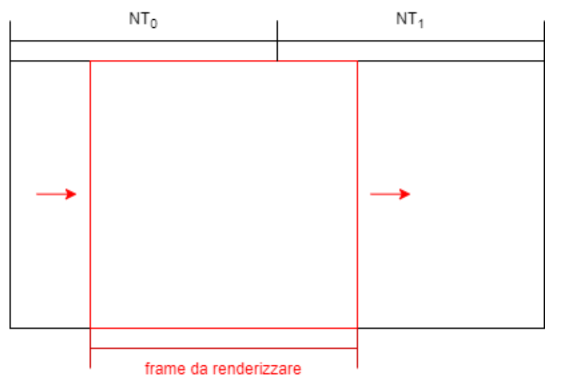
\includegraphics[width=270px, height=190px]{HOR_SCROLL.png}
\end{figure}\\
Il riquadro rosso individua nella fattispecie il frame da renderizzare, che però è posto tra $NT_0$ e $NT_1$. Questa cosa necessita che i tile, o meglio i \emph{pixel}, da renderizzare non devono partire dal punto più estremo in alto a sinistra del singolo nametable, bensì da un offset ben preciso, calcolato a partire dall'angolo estremo in alto a sinistra di uno dei due $NT$.\\
Per calcolare questo offset, prendiamo in esame una granatura per \emph{singolo tile}.\\
La granatura impone di calcolare l'offset con una formula del tipo:
\[
	y\cdot width+ x
\]
È tuttavia facile dimostrare che, scegliendo una stringa da 10 bit, e considerando la prima parte come \emph{coarse y} e la seconda come \emph{corase x}, abbiamo il nostro offset:
\begin{figure}[h]
\centering
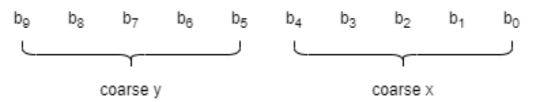
\includegraphics[width=275px, height=50px]{OFFSET_CALC.png}
\end{figure}\\
Aggiungendo due bit in testa, e arrivando quindi a una stringa di 12 bit totali, possiamo anche individuare qual è il nametable corrente nella fase di rendering.

In realtà, lo scrolling viene svolto con una granatura dell'ordine del pixel, e pertanto necessita che ci siano altre due variabili, nominate \emph{fine x} e \emph{fine y}, che specificano l'offset nel singolo tile.

A questo punto non rimane che legare i tile con i rispettivi attributi. Consideriamo che la attribute memory è grande $64 Byte$. In virtù di ciò, è possibile organizzarla come una matrice di $8\times8$ Bytes. Ogni byte fa riferimento a una regione di $4\times4$ tiles nella nametable corrispondente di dimensioni $32\times 30$ Bytes. In realtà, è possibile suddividere il singolo byte in quattro regioni da 2 bit ciascuna per poter individuare nella regione quattro sottoregioni da $2\times 2$ tiles. Per ognuna di queste sottoregioni è possibile specificare la palette desiderata, che coprirà quindi un'area pari a $16\times 16=256$ pixel.\\
Due bit sono sufficienti in virtù del fatto che le palettes destinate al rendering del background sono proprio 4 (sono sufficienti dunque solo 2 bit per trarre una delle 4 palette). A questo punto, l'associazione va a 2 a 2 con ogni blocchetto da $2\times 2$ tiles.
\begin{figure}[h]
\centering
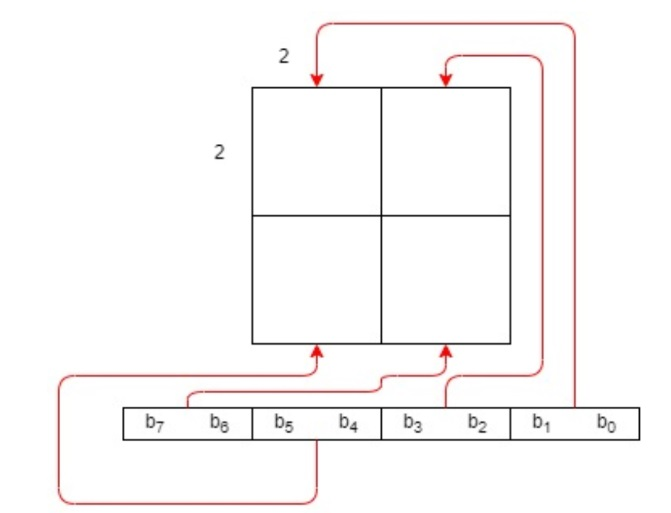
\includegraphics[width=300px, height=255px]{ATT_TILE_MAP.jpg}\\
\small\textbf{Mapping tra Byte dell'attribute memory e le varie regioni da essa rappresentata}
\end{figure}\\
C'è infine da considerare una cosa importante: così come per i tile, va specificato un \emph{attribute offset} per il relativo byte rappresentativo. Tuttavia, per \emph{coarse X} e \emph{coarse Y} sono sufficienti solo 3 bit ciascuno, risparmiando così 4 bit in totale, da poter usare per specificare le palette particolari da utilizzare per la singola regione indirizzata.
\paragraph{Gestione del rendering}
Per poter renderizzare un frame sono utili i cosiddetti \emph{loopy registers}. I loopy register sono dei registri interni alla PPU che consentono la lettura/scrittura della VRAM da parte della CPU, ma anche e soprattutto di supportare il rendering.

I loopy registers sono i seguenti:
\begin{itemize}
\item{
v: current VRAM (15 bit);
}
\item{
t: temporary VRAM (15 bit);
}
\item{
x: fine X scroll (3 bit);
}
\item{
w: first or second write toggle (1 bit).
}
\end{itemize}
Durante il rendering, la configurazione di t e v è la seguente:
\[
	yyyNNYYYYYXXXXX
\]
dove, a partire dal bit meno significativo, i primi 5 bit indicano l'offset rispetto all'asse orizzontale, i successivi 5 bit l'offset rispetto all'asse verticale, i successivi 2 la nametable scelta, e infine gli altri 3 l'offset rispetto all'asse verticale con granatura interna al tile.

Il punto importante è che, al di là della particolare configurazione di t e v, questi due registri sono influenzati pesantemente dalla comunicazione della CPU con la PPU tramite i vari registri. Ad esempio:
\begin{itemize}
	\item{
		Per una write su $\$2000$ con $d=......BA$, abbiamo:
		\[
			t = ...BA.........
		\]
	}
	\item{
		Per la first write su $\$2005$ con $d=HGFEDCBA$:
		\[
			t = .........HGFED
		\]
		\[
			x = CBA
		\]
		\[
			w = 1
		\]
	}
\end{itemize}
I loopy register vengono settati così, e partecipano attivamente al rendering dei frame.

Quando la PPU esegue, le sue operazioni dipendono dal suo passato. Ad esempio, se la PPU ha eseguito per un certo numero di cicli, allora essa si comporterà in maniera diversa, così come se essa ha eseguito per un certo numero di \emph{scanline}, si comporterà in maniera diversa.

In qualsiasi stato, tuttavia, essa farà uso dei loopy registers, ma non solo: per il rendering si rivelano necessari alcuni shift registers e altre variabili d'appoggio.

Tra gli shift registers ritroviamo:
\begin{itemize}
	\item{
	2 shift-registers di 16 bit ciascuno che memorizzano 2 tile; la parte più significativa contiene i primi 8 pixel da dover renderizzare, mentre la parte meno significativa l'altro tile pre-caricato.
	}
	\item{
	2 shift registers di 8-bit ciascuno che memorizzano gli attributi per il tile corrente.
	}
\end{itemize}
\clearpage
Gli shift registers si rivelano necessari poichè consentono di renderizzare un pixel alla volta. Concettualmente, quando si avvierà un nuovo ciclo nella parte di rendering grafico, si avrà una disposizione di questo tipo:
\begin{figure}[h]
\hspace*{-1.2cm}
\centering
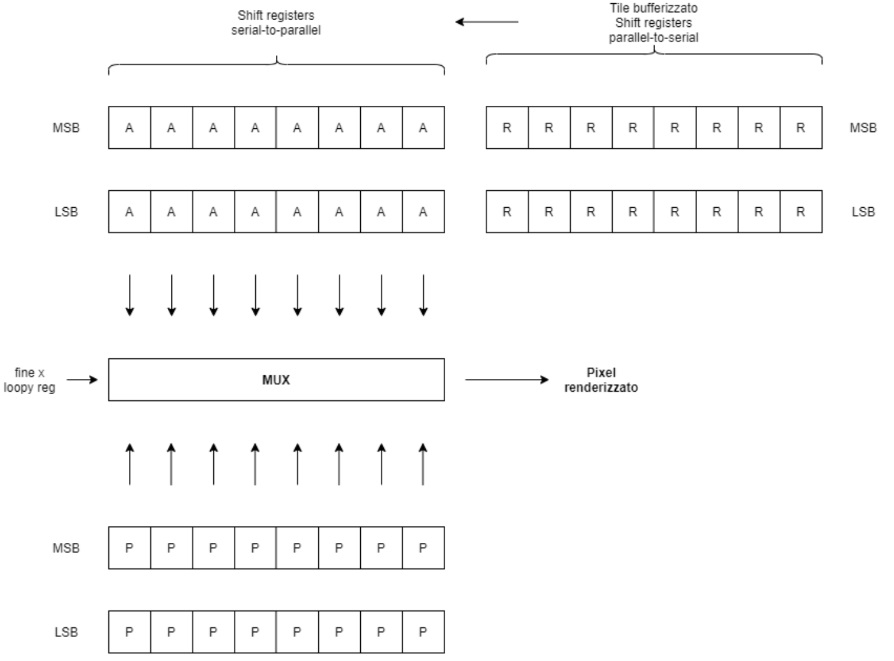
\includegraphics[width=450px, height=330px]{PIXEL_RENDERING_LOGIC.png}
\end{figure}\\
Concettualmente, supponiamo di disporre già una coppia di shift-registers pronti per essere renderizzati. Questi shift-registers sono quelli i cui singoli flip-flop sono etichettati con `A'. I valori di questi shift-registers si combinano con quelli dei corrispondenti attributi (shift-registers i cui singoli flip-flop sono etichettati con `P'), secondo il valore specificato dal loopy register \emph{fine x}: il multiplexer consente di selezionare il pixel da renderizzare avendo come segnale di abilitazione \emph{fine x}. 

Ovviamente quanto appena descritto fa riferimento alla situazione nominale per cui si dispone di tutti gli shift-registers riempiti, tuttavia la logica di controllo è più complessa di così; difatti si spenderanno cicli di clock della PPU a caricare i dati da immettere negli shift-registers, ad aggiornare la VRAM, ecc.

\subsubsection{Logica applicativa}
In vista di tutte queste informazioni appena enunciate, si rivela indispensabile il ritocco al \emph{System Domain Model} prima di poter procedere a svolgere le opportune scelte di design.
\begin{figure}[!h]
\hspace*{-3.3cm}
\centering
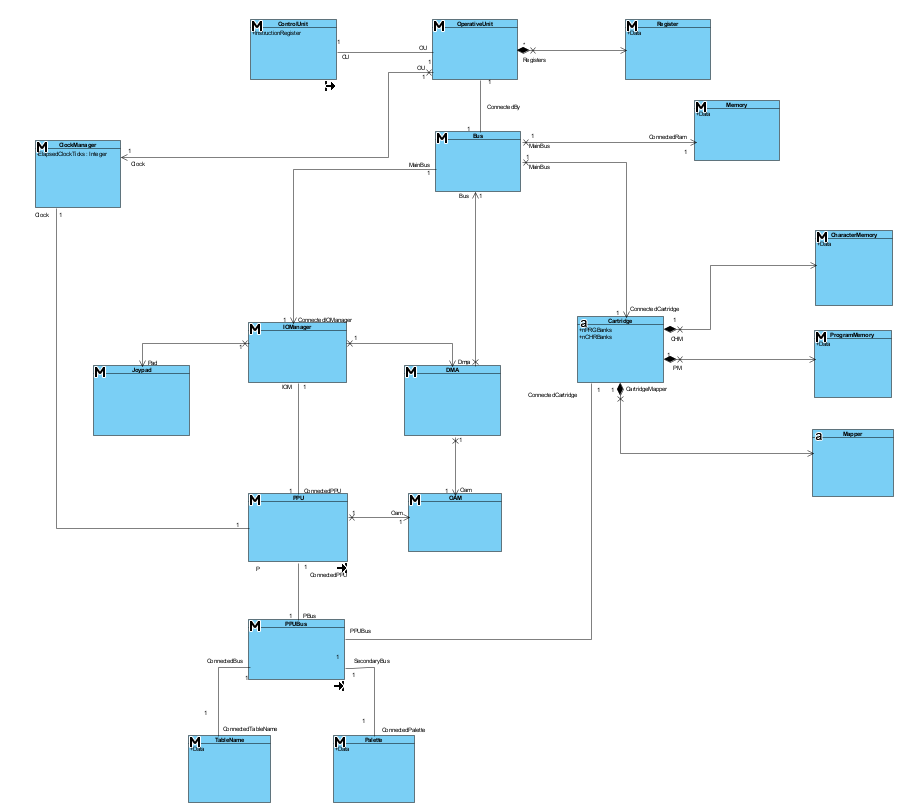
\includegraphics[width=525px, height=465px]{CD_DomainModel_2.png}
\end{figure}\\
Abbiamo l'introduzione di nuove, interessanti classi:
\begin{itemize}
\item{
	\emph{ClockManager}, che asserve al compito di gestire la tempificazione dei dispositivi. È a questa classe che la CPU afferisce per comprendere quando sia il suo `turno' di eseguire;
	ricordiamo in questa istanza che il NES è programmato perchè la PPU esegua \emph{3 volte più veloce}, quindi la CPU ha l'occasione di eseguire solamente ogni tre colpi di clock,
	a meno di situazioni eccezionali (come la lettura del DMA delle informazioni contenute all'interno della cartuccia);
}
\item{
	\emph{IOManager}, una classe che incapsula il controllo delle richieste redirezionate dal Bus verso una delle periferiche di I/O. Per mantenere basso accoppiamento, infatti, invece
	che portare il \emph{Bus} a collegarsi direttamente con tutte le periferiche di I/O, con questa periferica facciamo in modo che questa gestione sia nascosta al \emph{Bus}, il quale
	dovrà solamente passare la richiesta a questa classe;
}
\item{
	\emph{Joypad}, il dispositivo con cui l'utente comunica i comandi da inoltrare al videogioco in esecuzione;
}
\item{
	\emph{DMA}, la classe che rappresenta l'omonimo dispositivo fisico; sarà interessato nel trasferimento diretto dei dati da cartuccia verso l'OAM, una memoria interna alla PPU;
}
\item{
	\emph{OAM}, una memoria interna alla PPU che incapsula i dati inerenti ai cosiddetti `sprite'.
}
\end{itemize}
\clearpage
\subsection{Quarta iterazione}
\subsubsection{Premessa}
La quarta iterazione è stata l'ultima che è stata svolta prima di procedere alla consegna di tutto l'elaborato.\\
Questa iterazione è commessa a valle dell'aggiunta di molte feature per l'esecuzione del programma. Nella precedente iterazione il rendering grafico ha visto solamente il cosiddetto `rendering del background', che è un modo con cui si distingue il rendering di elementi allo sfondo dei videogame che vengono eseguiti sull'emulatore. In questa iterazione particolare attenzione si porrà sul rendering grafico del cosiddetto `foreground', ossia essenzialmente di tutti quegli elementi grafici dinamici che intervengono nell'esecuzione di un videogioco. Ci sono anche altri elementi al contorno che hanno richiesto, per questa iterazione, un perfezionamento.
\subsubsection{Gestione della lista dei programmi}
È d'interesse per la corrente iterazione sviluppare la gestione della lista dei programmi a disposizione per l'utente mediante le consuete operazioni CRUD inoltrabili verso il Database. La particolarità sta nel fatto che bisognerà consentire la comunicazione tra gli elementi dell'architettura destinati alla gestione dei file su File System: ad esempio, per l'inserimento di un programma dal File System, bisognerà dapprima caricare i dati dal File System, e imprimerli successivamente nel Database in maniera opportuna. 

\subsubsection{PPU - foreground }
Per foreground intendiamo il rendering a schermo dei personaggi, o in generale degli sprites che si muovono sul background. L’idea di base per il rendering del foreground è la stessa di quella del background ma in questo caso bisogna fare attenzione a dei particolari quali
\begin{itemize}
\item{
	\emph{Sprites}, cosa sono e dove vengono memorizzati;
}
\item{
	\emph{Sprite Rendering}, visualizzazione e posizionamento;
}
\item{
	\emph{Sprite Orientation}, orizzontale e verticale;
}
\item{
	\emph{Collision Detection};
}
\end{itemize}
\paragraph{Sprites}
Uno sprite rappresenta un Tile del foreground ed è caratterizzato da 4 Byte di informazioni quali
\begin{itemize}
\item{
	\emph{Coordinata Y};
}
\item{
	\emph{Tile ID};
}
\item{
	\emph{Attribute}, (Pritority, palette, orientation);
}
\item{
	\emph{Coordinata X};
}
\end{itemize}
Memorizzati in quest’ordine, queste informazioni sono presenti in una memoria propria della PPU chiamata OAM (Object Attribute Memory). L’OAM è una memoria di 256 Bytes contente 64 possibili sprites. Per popolare il più rapidamente possibile la memoria della PPU, invece di passare ogni volta per la CPU, viene utilizzato un dispositivo chiamato DMA (Direct Memory Access) che prende il controllo del BUS mettendo in pausa la CPU e che copia un’intera pagina di memoria (256 Bytes) dal BUS della CPU nell’ OAM. Questa tecnologia nella pratica incrementa di 4 volte la velocità di trasferimento dei dati.
\paragraph{Sprite Rendering}
Il problema principale della stampa degli sprites è che essi possono trovarsi in qualsiasi punto dello schermo in momenti diversi, per cui ci dobbiamo chiedere quando la PPU si rende conto che c’è bisogno di stampare uno o più sprites. Ricordiamo che i pixel vengono renderizzati riga per riga utilizzando dei contatori di colonna (i Cycles) e di riga (le scanlines), per cui alla fine di ogni riga renderizzata a schermo andremo a controllare se nella prossima riga sarà presente uno sprite da disegnare. \\
Prima di tutto bisogna capire quale e se è presente uno sprite da disegnare nella prossima riga, confrontando la coordinata Y degli sprite nell’OAM con quella dello schermo (cioè lo scanline). Se la differenza è compresa tra 0 e l’altezza dello sprite (8 o 16 a seconda della modalità scelta) allora dovrà essere stampato quel determinato sprite.\\
Appurata l’esistenza dello sprite sullo schermo, dobbiamo ricavare il Byte da disegnare nella prossima riga e la sua posizione. Per farlo iniziamo a renderizzare la riga successiva e ad ogni cycle andiamo a sottrarre 1 alla coordinata x dello sprite da disegnare a schermo, così che quando la coordinata x sarà pari a 0 vorrà dire che è arrivato il momento di disegnare lo sprite.  \\
In tutto questo bisogna fare attenzione al massimo numero di sprite renderizzabili in un frame. Il NES è in grado di renderizzare al massimo 8 sprites per frame e in caso si cerchi di renderizzare più sprites verrà alzato un bit di segnalazione nel registro di Stato della PPU.\\
Un'altra condizione interessante si verifica quando ci sono più sprites nella stessa posizione. Bisogna in quel caso gestire una priorità e per farlo semplicemente ci si appoggia alla posizione degli sprites nell’OAM. In particolare, gli sprites posizionati nelle locazioni puntate da indirizzi più bassi dell’OAM sono più prioritari per cui mi basterà prelevare lo sprite più prioritario cercando dall’alto verso il basso nell’OAM.
\paragraph{Sprite Orientation}
Data la limitata quantità di memoria del NES, esso implementa una tecnica per specchiare orizzontalmente o verticalmente uno sprites in modo da non dover memorizzare più sprites per lo stesso personaggio ma con orientamento diverso. In particolare, nella Cartridge leggeremo l’orientamento del personaggio e in caso esso dovrà essere specchiato orizzontalmente, andremo a invertire i bit dello sprite in ogni riga. Se invece il personaggio dovrà essere specchiato verticalmente allora basterà invertire gli indirizzi che puntano alle righe dello sprite. 
\paragraph{Collision Detection}
Durante l’andamento di un videogioco potremmo voler tenere dei dati costanti a schermo durante lo scrolling. Per gestire questo comportamento il NES implementa la Collision detection, cioè utilizza un flag detto “SpriteZeroHitDetection” che permette di sincronizzare CPU e PPU.  Quando si verifica una collisione con lo Sprite Zero esso modificherà il flag e indicherà alla CPU in quale parte dello schermo si sta permettendo alla CPU di decidere quale parte dello schermo renderizzare in maniera costante e indipendente dallo scrolling. Questo permette per esempio di avere una barra di stato costante in alto sullo schermo, mentre il resto si muoverà tramite la tecnica di scrolling discussa precedentemente.
\clearpage

\section{Design funzionale/non-funzionale}
Una volta svolto il workshop dei requisiti, e quindi arrivati ad analizzare questi ultimi, il design del sistema è volto a soddisfare tali requisiti, che siano essi funzionali oppure non funzionali. Dettagliamo in questo caso le scelte svolte per ogni iterazione.
\subsection{Prima iterazione}
Nella prima iterazione siamo particolarmente interessati a sviluppare la parte critica che ha previsto l'implementazione delle classi concettuali esposte nel domain model; prima di ciò, tuttavia, ha dovuto seguire un'approfondimento dell'architettura da adottare per realizzare l'emulatore.
\subsubsection{Architettura logica dell'emulatore}
L'architettura che è stata scelta per sviluppare l'emulatore è un'architettura a livelli; non solo: avendo appreso che la logica applicativa del sistema prevede l'interpretazione di istruzioni, abbiamo scelto, per il layer relativo alla logica applicativa, di applicare uno stile a interprete, privato, tuttavia, del layer di interfacciamento verso l'esterno, in quanto le istruzioni vengono continuamente determinate tramite la manipolazione del Program Counter nell'esecuzione di un certo programma. In ogni caso, il diagramma modulare risultante è mostrato nella seguente pagina.
\begin{figure}[t]
\centering
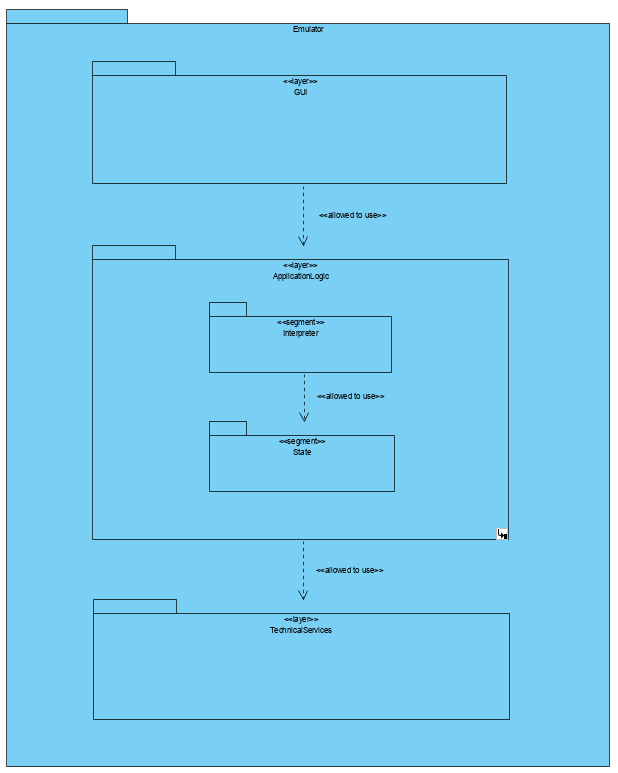
\includegraphics[width=375px, height=468px]{CD_Emulator_Architecture.png}\\
\small\textbf{CD\_Emulator\_Architecture}
\end{figure}
\clearpage
La scelta a livelli è motivata perchè innanzitutto consente già di mappare i requisiti che coinvolgono la gestione eventuale di una lista di programmi mediante l'interfacciamento ai servizi esposti dal livello \emph{Technical Services}, l'interazione dell'utente mediante un'interfaccia grafica messa a disposizione da parte del package \emph{GUI}, e l'inquadramendo della logica applicativa (in cui è contenuta un'ulteriore stratificazione a livelli dato dallo stile a interprete) nel package \emph{Application Logic}.\\
I requisiti non funzionali anche vengono in parte soddisfatti: un'architettura a livelli evolve facilmente, le responsabilità sono tra loro ben distinte, il lavoro è facilmente distribuibile nel team, e qualora avvenissero dei cambiamenti anche per i requisiti già sviluppati, la loro integrazione non sarebbe difficoltosa data l'indipendenza tra i vari layer e il tracciamento semplice del flusso di controllo e dei flussi di dati. È particolarmente importante che la scelta architetturale presti a una facile \emph{modificabilità}: essendo il sistema sconosciuto per molte parti, che verranno successivamente approfondite, è di fondamentale importanza disaccoppiare tra loro le varie entità modulari.

\subsubsection{Raffinamento della dinamica di EseguiProgramma}
Siamo successivamente passati al raffinamento dell'architettura logica mediante l'aggiunta di classi software, ispirandoci, soprattutto per quanto riguarda il livello di dominio applicativo, alle classi già modellate in precedenza. Prima di ciò, tuttavia, è bene dire che il raffinamento della dinamica del caso d'uso EseguiProgramma è stato determinante per la corretta modellazione a livello di design dell'annesso class diagram. Innanzitutto, poichè lo stile a interprete si configura per essere altamente dinamico, dipendendo essenzialmente dallo stato interno del processore, ma anche dalla particolare istruzione ottenuta in ingresso, è stato più facile descrivere questa sottoparte di tutto il caso d'uso attraverso uno \emph{state diagram}, che è presentato nella successiva pagina.

Lo state diagram descrive essenzialmente il comportamento dell'unità di controllo durante tutta l'esecuzione del programma; si può facilmente annoverare questo comportamento tra quelli tipici di una CPU, ossia riconducibile al ciclo di Von Neumann. Nel nostro caso, la descrizione calza a pennello, e rende anche molto più facile, rispetto che a un sequence diagram, la descrizione del comportamento dell'unità di controllo. Ricordiamo, infatti, che i vari codici operativi, modi d'indirizzamento, ecc. portano ad avere un comportamento estremamente variegato, che è bene descrivere in maniera indipendente per poter effettivamente rendere i diagrammi usufruibili per la parte implementativa. 
\clearpage
\begin{figure}[h]
\centering
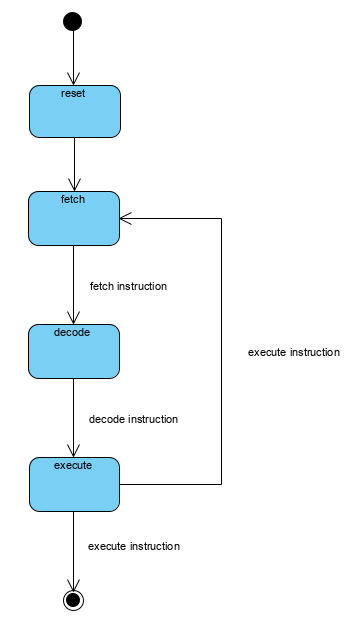
\includegraphics[width=200px, height=352px]{SD_ControlUnit.png}\\
\small\textbf{SD\_ControlUnit}
\end{figure}

Interessante, in questo contesto, è anche mettere enfasi sul fatto che se non si adoperasse la programmazione concorrente, l'unico thread che eseguirebbe il programma renderebbe l'interfaccia completamente unresponsive, il che va contro i requisiti non-funzionali che sono stati imposti all'inizio del progetto. Ciò lascia spazio a una modellazione un po' più articolata delle varie \emph{attività} che vengono svolte nel contesto dell'esecuzione del programma, ma anche in parte per la visualizzazione dello stato dell'architettura.\clearpage Consideriamo, dunque, l'activity diagram:
\begin{figure}[h]
\hspace*{-1cm}
\centering
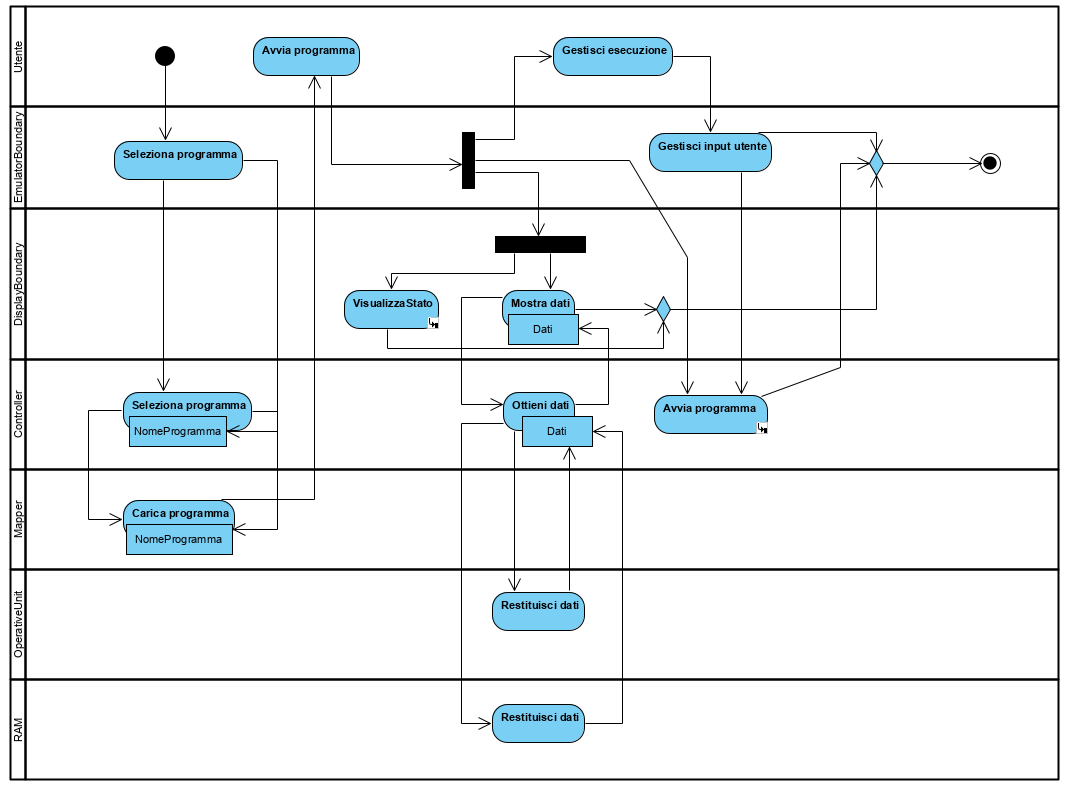
\includegraphics[width=400px, height=295px]{AD_EseguiProgramma.png}\\
\small\textbf{AD\_EseguiProgramma}
\end{figure}


Gli activity diagram sono particolarmente utili poichè consentono di visualizzare concretamente dov'è che ci sono più flussi di controllo concorrenti, e quindi aiutano anche a sviluppare un design più vicino all'implementazione. Le varie attività sono descritte in termini generali, e si può già scorgere un accenno di quelle che sono altre feature messe a disposizione dal sistema, come la visualizzazione dello stato e la gestione degli input utente. 

A questo punto è possibile arrivare a una descrizione modulare della nostra architettura raffinando ciò di cui già disponiamo. Enunciamo in questa sede tutti i design pattern che vengono adoperati:
\begin{itemize}
	\item{
		\emph{State pattern}, adoperato per descrivere i vari stati che attraversa la \emph{ControlUnit};
	}
	\item{
		\emph{Facade pattern}, per garantire un unico punto di accesso a un layer attraverso un singolo oggetto che espone l'interfaccia di quel dato layer;
	}
	\item{
		\emph{Singleton pattern}, ampiamente utilizzato in tutto il progetto, il pattern si rivela fondamentale poichè il peculiare contesto in cui è immerso l'intero sistema
		prevede un numero di istanze limitato, spesso pari proprio a 1, delle classi in gioco. Oltretutto, facendo in modo che l'accesso agli oggetti sia fatto attraverso
		un'istanza statica, consente agli elementi di poter mantenere il proprio stato per tutta la durata del programma (si pensi alla \emph{Cartridge} che si prevede sarà acceduta
		da più oggetti e bisogna dunque fare in modo che il suo stato sia persistente per tutta la durata del programma).
	}
	
\end{itemize}
Rappresentiamo dunque in questa istanza una piccola parte del class diagram nella presente iterazione per mostrare effettivamente tutti i design pattern utilizzati:
\begin{figure}[h]
\hspace*{-4.3cm}
\centering
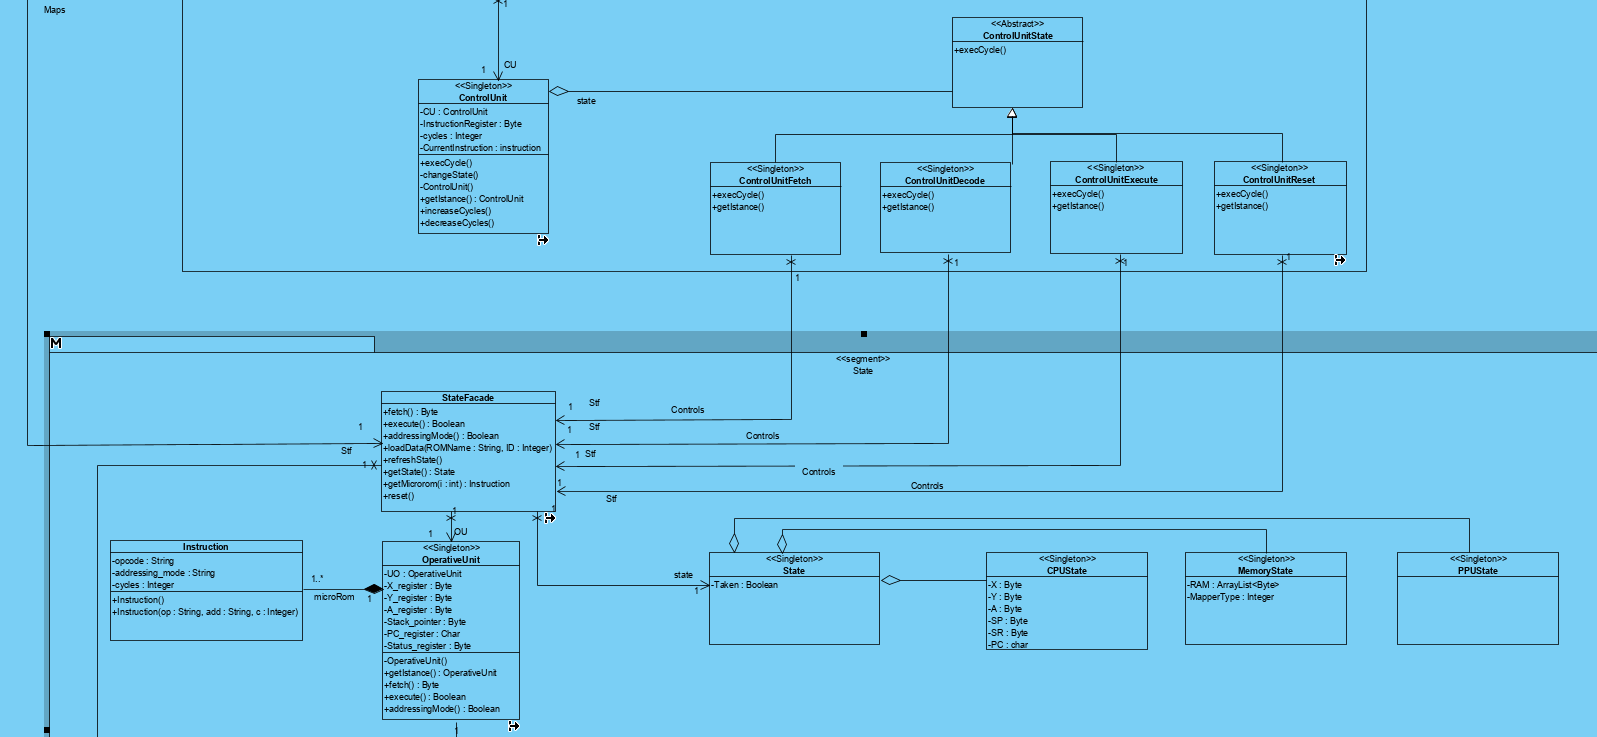
\includegraphics[width=600px, height=277px]{CD_Emulator_0.png}
\end{figure}\\
Dando dei piccoli commenti, possiamo dire che sono stati apposti gli stereotipi alle classi laddove è stato ritenuto necessario; si vedono oltretutto delle nuove classi che nel \emph{domain model} non sono state modellate, come la classe \emph{State} e quella \emph{Instruction}; non appare, oltretutto, la classe \emph{Register}. Questa cosa non è propriamente sbagliata: le classi del domain model sono solamente concettuali; le classi qui raffigurate si avvicinano già all'implementazione, e saranno specialmente utili per guidare i progettisti alla programmazione di quanto progettato.\\
Nel piccolo spezzone mostrato non è rappresentato, ma abbiamo anche introdotto un'ulteriore layer, denominato `Controller', che incapsula le responsabilità demandate alla gestione degli input utente trasportati dalla GUI verso gli altri livelli del sistema.

A questo punto, conosciuta la dinamica, conosciuto il class diagram, possiamo mostrare uno dei tanti sequence diagram che popolano il modello dinamico del nostro sistema software:
\begin{figure}[h]
\hspace*{-1cm}
\centering
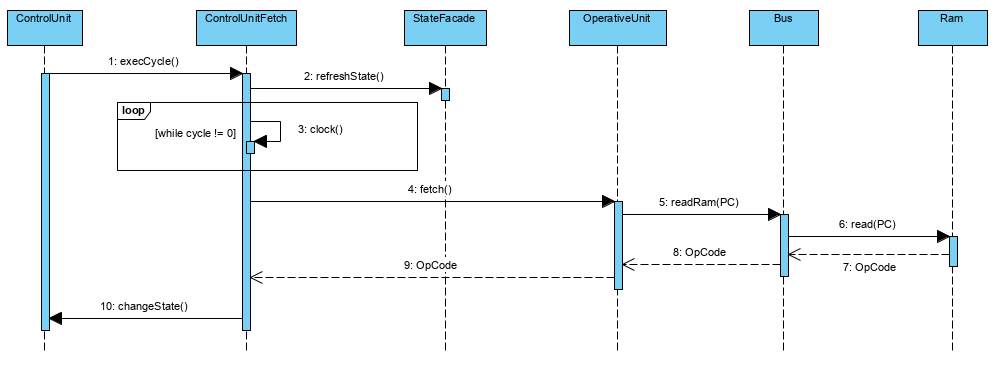
\includegraphics[width=350px, height=127px]{SQD_fetch_execCycle().png}\\
\small\textbf{SQD\_fetch\_execCycle()}
\end{figure}\\
Questo diagramma esplica il comportamento della \emph{ControlUnit} qualora essa si trovi nello stato `fetch'; nel modello, per ogni stato, abbiamo modellato lo specifico diagramma di sequenza.
\clearpage
\subsubsection{Vista componenti\&connettori}
Come ben noto, la vista modulare non dà informazioni rilevanti a riguardo degli elementi costitutivi del sistema a run-time; è necessario sviluppare dei diagrammi, o meglio fornire delle viste del sistema software, che possano in qualche modo rappresentare quali sono le entità che figureranno nel sistema a run-time. I diagrammi scelti sono quelli che vanno sotto al nome di diagrammi dei componenti; presentiamo dapprima il cosiddetto \emph{catalogo}, che fornisce tutti i vari \emph{tipi} di componenti che intervengono nel sistema, e successivamente faremo vedere un diagramma dove i vari componenti si configurano per essere delle istanze dei tipi più genericamente definiti nel catalogo. 

Premettiamo, innanzitutto, di star usando uno stile \emph{shared-data}, dove esistono dei componenti, definiti \emph{repository}, con cui i componenti software del sistema interagiscono per recuperare dati memorizzati su una fonte condivisa; ciò in virtù del fatto che l'assemblatore presente nel NES pubblica, eventualmente, dei programmi compilati su una fonte condivisa con l'emulatore. Ma anche, è previsto che l'emulatore possieda un proprio repository personale su cui memorizzare dei programmi; lo stile scelto, pertanto, si presta bene allo scopo del progetto. \clearpage
Osseviamo dunque il catalogo dei componenti:
\begin{figure}[h]
\centering
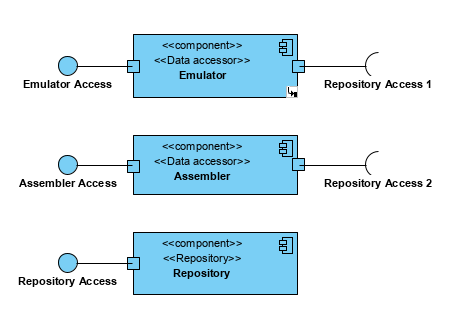
\includegraphics[width=240px, height=175px]{CMPD_NES_Catalogue.png}\\
\small\textbf{CMPD\_NES\_Catalogue}
\end{figure}
E quindi il successivo diagramma dei componenti:
\begin{figure}[h]
\centering
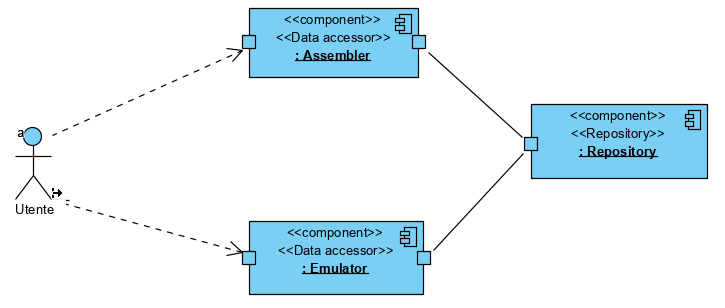
\includegraphics[width=300px, height=125px]{CMPD_NES.png}\\
\small\textbf{CMPD\_NES}
\end{figure}
\clearpage
\subsection{Seconda iterazione}
\subsubsection{Architettura logica dell'emulatore}
Per quanto concerne l'architettura logica abbiamo provveduto massicciamente a migliorare la modellazione degli aspetti statici e dinamici di quanto avevamo già sviluppato, correggendo gli errori che sono emersi da un'analisi più approfondita del dominio, e prevedendo nuove funzionalità. Ovviamente le strutture che abbiamo previsto per la prima iterazione sono rimaste integre, e il sistema si è rivelato davvero facilmente estendibile, soprattutto per la scelta dei design pattern che abbiamo fatto nella prima iterazione.
\paragraph{Aspetti statici: ApplicationLogic}
Dal punto di vista statico abbiamo arricchito il layer \emph{ApplicationLogic}, come ad esempio l'aggiunta di un nuovo stato per la \emph{ControlUnit}, e organizzando per ogni segmento un'interfaccia per favorire la distribuzione dei compiti tra i membri del team. Come prima, non faremo vedere tutto il diagramma delle classi perchè è troppo folto e denso di concetti, ma per far intravedere gli sviluppi, mostriamo nella pagina successiva un paio di fotografie che palesano le modifiche e le aggiunte al layer \emph{ApplicationLogic}
\begin{figure}[!h]
\vspace*{-4cm}

\centering
	\begin{subfigure}{600px}
	\hspace*{-4.3cm}
	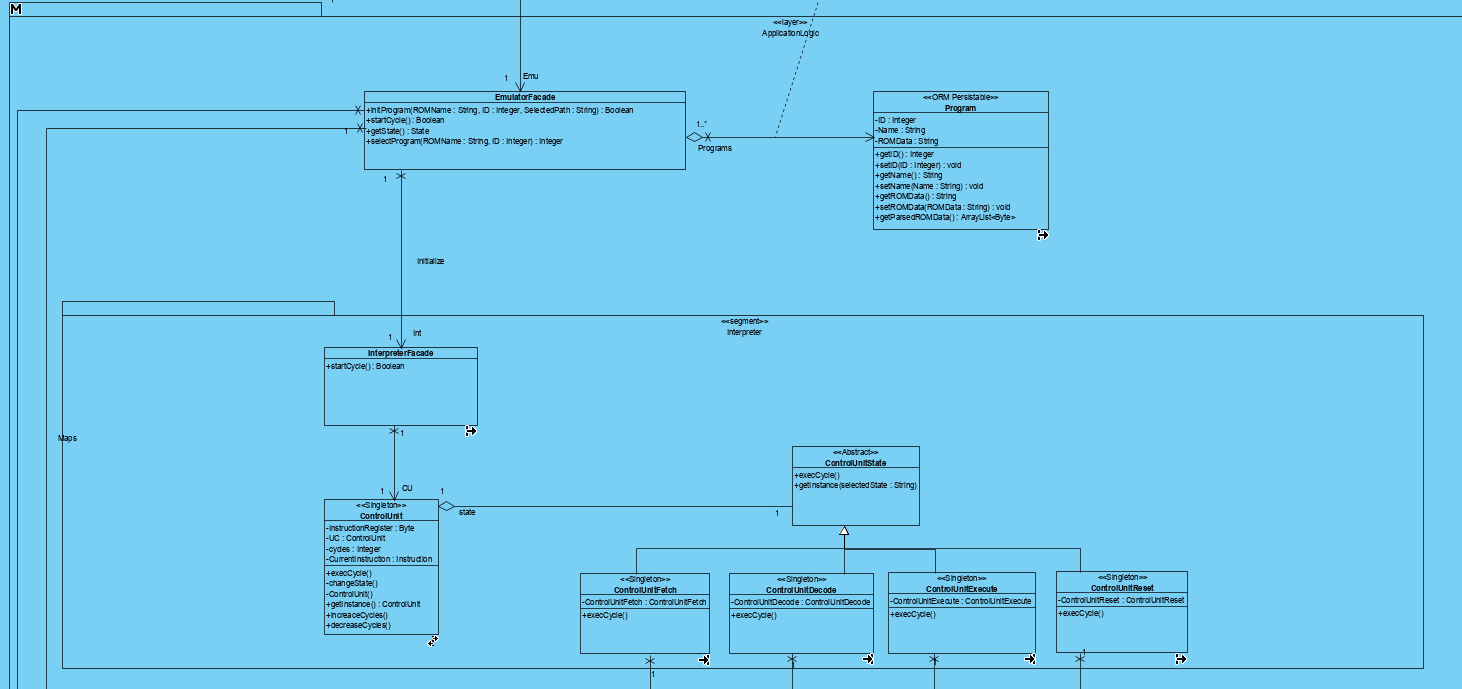
\includegraphics[width=600px, height=281px]{CD_Emulator_1.png}\\
	\end{subfigure}
	\begin{subfigure}{600px}
	\hspace*{-4.3cm}
	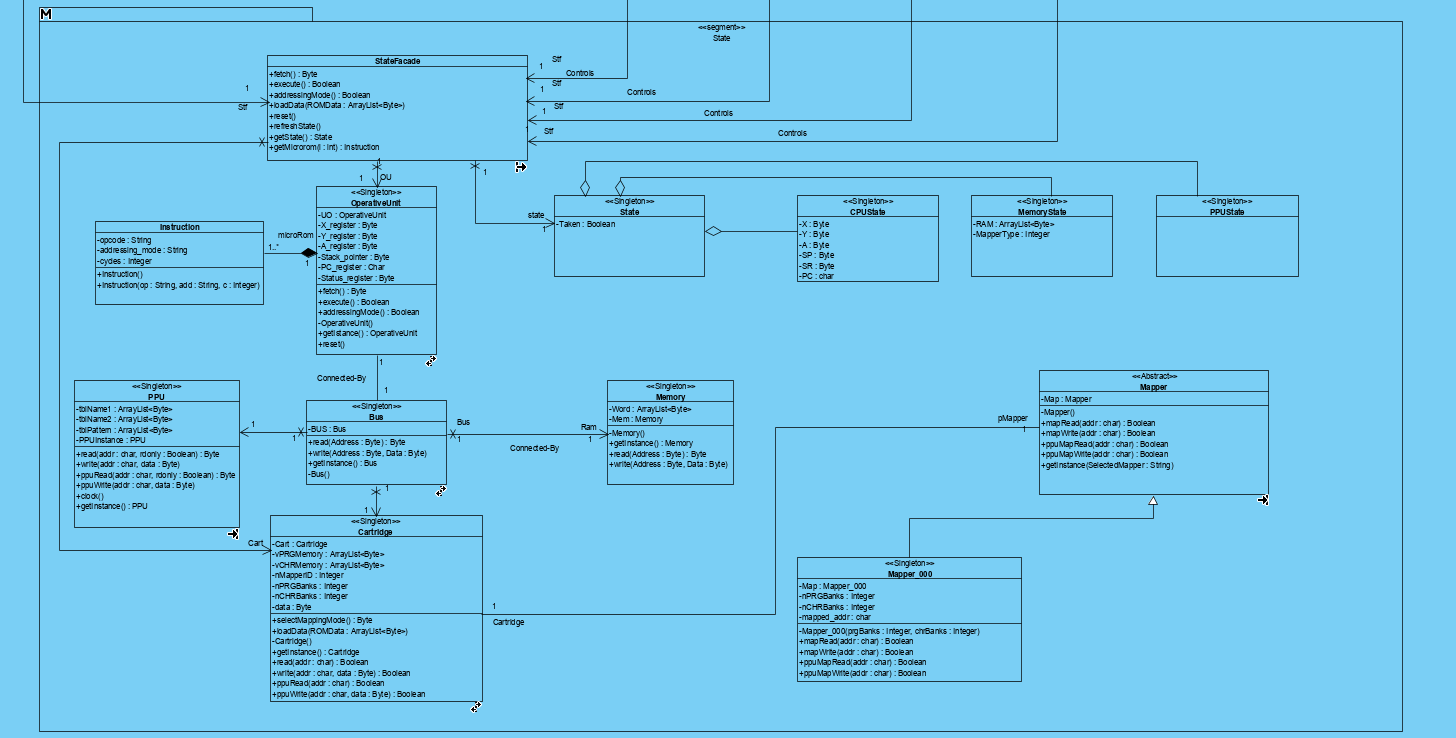
\includegraphics[width=600px, height=281px]{CD_Emulator_2.png}\\
	\end{subfigure}
	\small\textbf{CD\_Emulator}
\end{figure}\\
Come detto, tra le modifiche più significative rientra l'aggiunta di un nuovo stato per la \emph{ControlUnit}, la riorganizzazione dei collegamenti tra classi all'interno del segmento \emph{State}, l'aggiunta di polimorfismo per determinare dinamicamente il mapper della cartuccia che viene caricata.
\clearpage
\paragraph{Aspetti statici: TechnicalServices}
Obbiettivo della corrente iterazione è, ricordiamo, fare in modo che il caricamento di una qualsiasi cartuccia avvenga correttamente. Notiamo una classe importante, che va sotto al nome di \emph{Program}. Program è una classe che incapsula le informazioni a riguardo di tutte le cartucce di cui l'utente dispone e che è interessato a caricare. Attenzione: il programma non va inteso come la cartuccia \emph{innestata} all'interno dell'emulatore, ma è inteso come il programma che viene recuperato dal File System o dal Database, e quindi caratterizzato per avere un ID, un Nome, e i dati binari convertiti sottoforma di stringa (attraverso un'opportuna conversione). La classe rispecchia, di fatto, l'entità presente all'interno del Database relazionale, che mantiene tre colonne, nominate allo stesso modo di come sono stati nominati gli attributi della classe stessa. Lo stereotipo \emph{ORM Persistable} sta proprio a indicare che quella classe rispecchia un'entità del modello relazionale, direttamente mappata con gli oggetti all'interno del nostro sistema software.\\
Poichè è la classe \emph{EmulatorFacade} che si interfaccia direttamente con il Database per recuperare i dati relativi ai programmi, abbiamo scelto di modellare una relazione di contenimento tra \emph{EmulatorFacade} e la classe \emph{Program}: è l'EmulatorFacade, pertanto, la classe \emph{information expert} degli oggetti appartenenti alla classe \emph{Program}, e sarà essa responsabile della loro creazione e della interlocuzione con gli elementi di questa classe. Osserviamo, pertanto, la parte del class diagram sviluppato inerente all'interfacciamento con il File System e il Database nella successiva pagina.
\begin{figure}[!h]
\hspace*{-4.3cm}
\centering
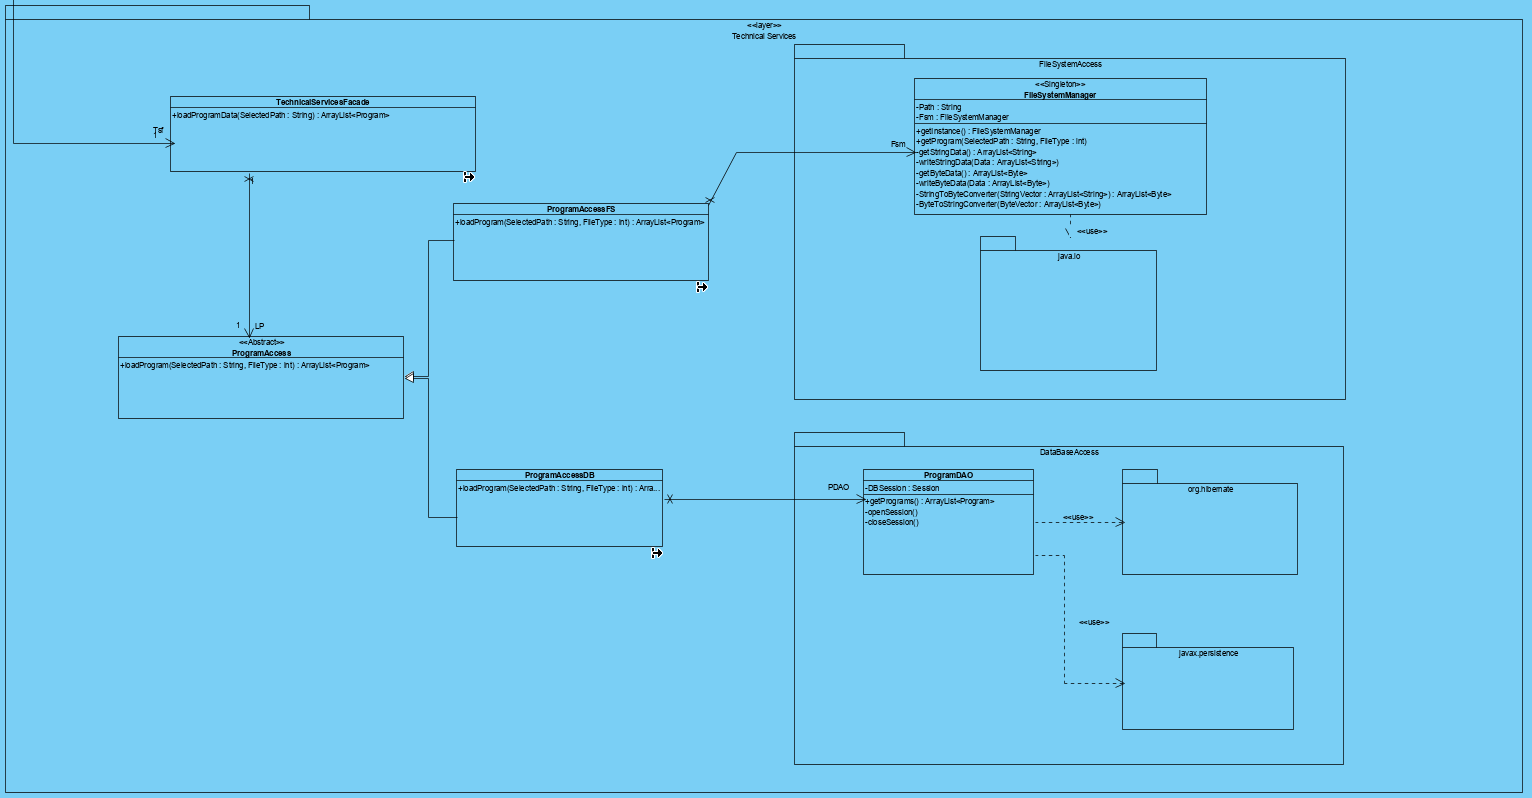
\includegraphics[width=600px, height=315px]{CD_Emulator_3.png}\\
\small\textbf{CD\_Emulator}
\end{figure}\\
Abbiamo che, mediante un'opportuna gestione del polimorfismo, il \emph{TechnicalServicesFacade} potrà decidere di scegliere di usufruire dei servizi particolarizzati per l'accesso al Database oppure al FileSystem. Qualora si fosse interessati a ottenere informazioni dal Database, la classe \emph{ProgramAccessDB} interloquia con la classe \emph{ProgramDAO} che si occupa di aprire una connessione col database e recuperare i dati da quest'ultimo, mentre qualora si fosse interessati a ottenere informazioni dal File System, la classe \emph{ProgramAccessFS} interloquia con la classe \emph{FileSystemManager} che si occuperà di leggere i dati. Ovviamente la lettura dei dati dal File System necessita di avere accortenze: bisogna essere compliant con quanto già è stato analizzato in questa iterazione, e quindi valgono i discorsi sui formati, sulla conversione, ecc. Ciò motiva anche la presenza di molte funzioni all'interno di questa classe, che assolvono proprio al compito di convertire opportunamente i dati che vengono tratti dal File System.
\clearpage
\paragraph{Aspetti statici: GUI }

Passati ad una fase di design, abbiamo spinto la progettazione verso una prima modellazione statica del problema.\\
Come prima cosa il package UI è stato arricchito di altri 2 sottopackage, rispettivamente \emph{EmulatorBoundaryPackage} e \emph{DisplayBoundaryPackage}. \\
Questi due package serviranno a separarare secondo approccio modulare le due entità di confine, dove la prima avrà un ruolo di controllo verso la seconda, che si comporterà invece più come una vista che altro.

è chiaro allora che entrambe le entità debbano essere realizzate come delle classi fra loro associate, dove l'EmulatorBoundary avrà una responsabilità di \emph{Creator} nei confronti del display Boundary.\\
Ci aspettiamo che l'emulator boundary esponga diversi metodi per l'inizializzazione dei suoi componenti e per l'avvio del programma. In realtà in questa fase sono già state impostate delle funzionalità per la creazione dei flussi concorrenti, seppur non ancora approfondite.

Al contempo è stata aggiunta una classe di configurazione \emph{UIConfiguration} con la quale tener traccia sia della modalità (da inoltrare al display boundary) sia dei parametri relativi al programma da caricare.\\
Tale struttura di principio è costruita per essere espandibile, andando di pari passo con il tipo di configurazione che vorremo fornire in futuro all'utente.

Naturalmente è fondamentale che l'Emulator Boundary comunichi con il controllore sottostante per poter richiamarne i servizi sia per il caricamento del programma che per il suo avvio.\\
A questo punto è possibile spendere due parole sulla progettazione ancora preliminare del package DisplayBoundary. Infatti allo stato attuale ci interessiamo unicamente della sua creazione, e non ancora del suo effettivo comportamento; ciò nonostante abbiamo preparato una piccola impalcatura relativa ai vari frame che tale display potrà mostrare su richiesta, \emph{on demand}, dell'utente, tramite opportune iterazioni.

Per concludere il discorso relativo alla progettazione della GUI in questa iterazione, va specificato l'esplicito collegamento al package \emph{JavaSwing}, che rappresenta il framework che abbiamo stabilito di usare.\\

\begin{figure}[!h]
\hspace*{-4.3cm}
\centering
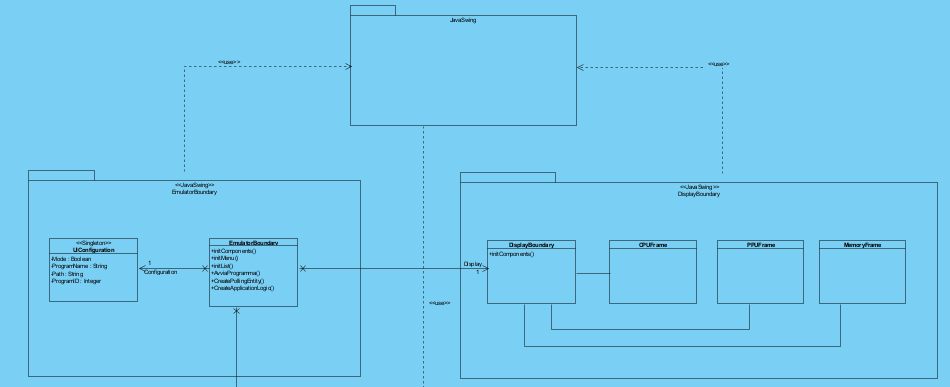
\includegraphics[width=600px, height=260px]{CD_UI.png}
\small\textbf{Class Diagram di design per la GUI, durante la seconda iterazione}\\
\end{figure}


\clearpage
\subsubsection{Raffinamento della dinamica di EseguiProgramma}
A tutte le modifiche svolte dal punto di vista statico, è coinciso ovviamente un raffinamento della dinamica di EseguiProgramma.

Innanzitutto, è stato modificato il diagramma degli stati che descrive l'evoluzione della \emph{ControlUnit}, aggiungendovi uno stato di \emph{reset}, che consente di impostare l'architettura a uno stato noto (volendo dare una vista più a basso livello, lo stato di reset prevede di impostare tutti i registri della \emph{OperativeUnit} a dei valori iniziali, e far partire il registro \emph{PC} da un indirizzo letto a partire dalle locazioni di memoria 0xFFFC e 0xFFFD):
\begin{figure}[h]
\centering
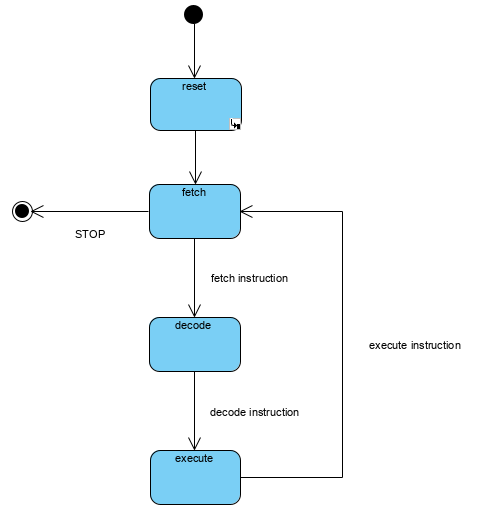
\includegraphics[width=270px, height=290px]{SD_ControlUnit_1}
\end{figure}\\
Da notare anche che è stato cambiato il punto di uscita, che adesso è impostato come possibilità per lo stato di \emph{fetch}, piuttosto che \emph{execute}. Il tutto è documentato nei vari diagrammi che sono stati sviluppati per ogni stato. Volendo darne una vista, osserviamo, anche per comparazione rispetto a quello della precedente iterazione, quello per la fetch appena nella prossima pagina.
\begin{figure}[!h]
\hspace*{-1.2cm}
\centering
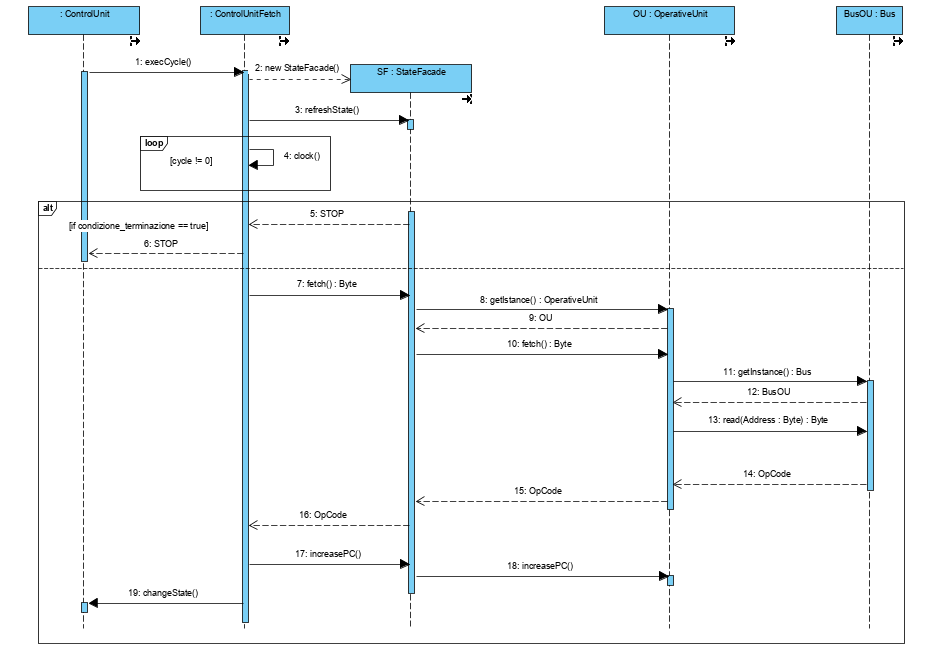
\includegraphics[width=425px, height=303px]{SQD_fetch_execCycle()_1.png}\\
\small\textbf{SQD\_fetch\_execCycle()}
\end{figure}\\
A questo punto possiamo anche mostrare il sequence diagram più generale che comincia a mostrare a un livello di dettaglio più ampio il sequence diagram annesso al caso d'uso \emph{EseguiProgramma}. Ovviamente è molto complesso, e le sue parti sono state combinate con altre viste, così come abbiamo ispezionato finora, ma il sequence riesce a fornire una visione abbastanza completa del punto di inizio del caso d'uso, e del punto di fine. Mostriamo il sequence nella successiva pagina, suddiviso in due parti.
\begin{figure}[!h]
\vspace*{-4cm}

\centering
	\begin{subfigure}{600px}
	\hspace*{-4.3cm}
	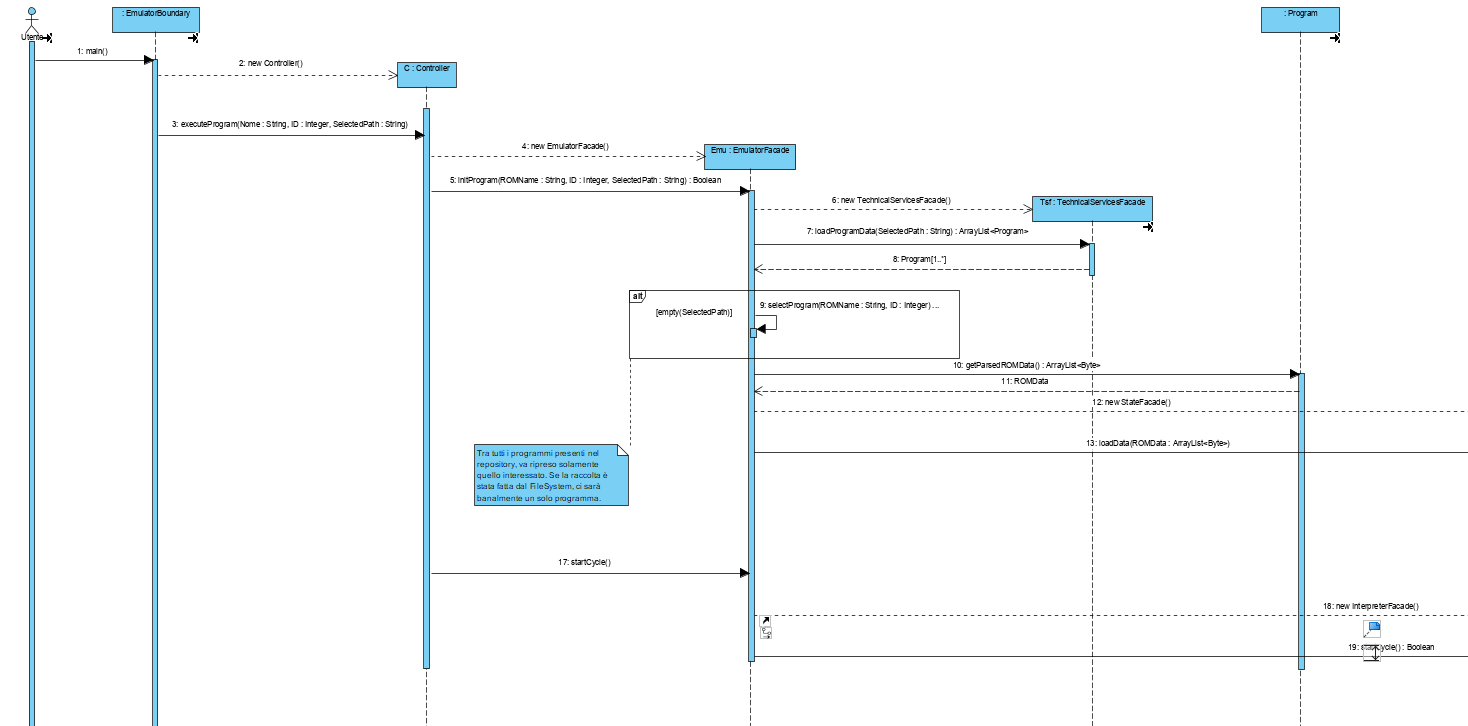
\includegraphics[width=600px, height=281px]{SQD_EseguiProgramma_1.png}\\
	\end{subfigure}
	\begin{subfigure}{600px}
	\hspace*{-4.3cm}
	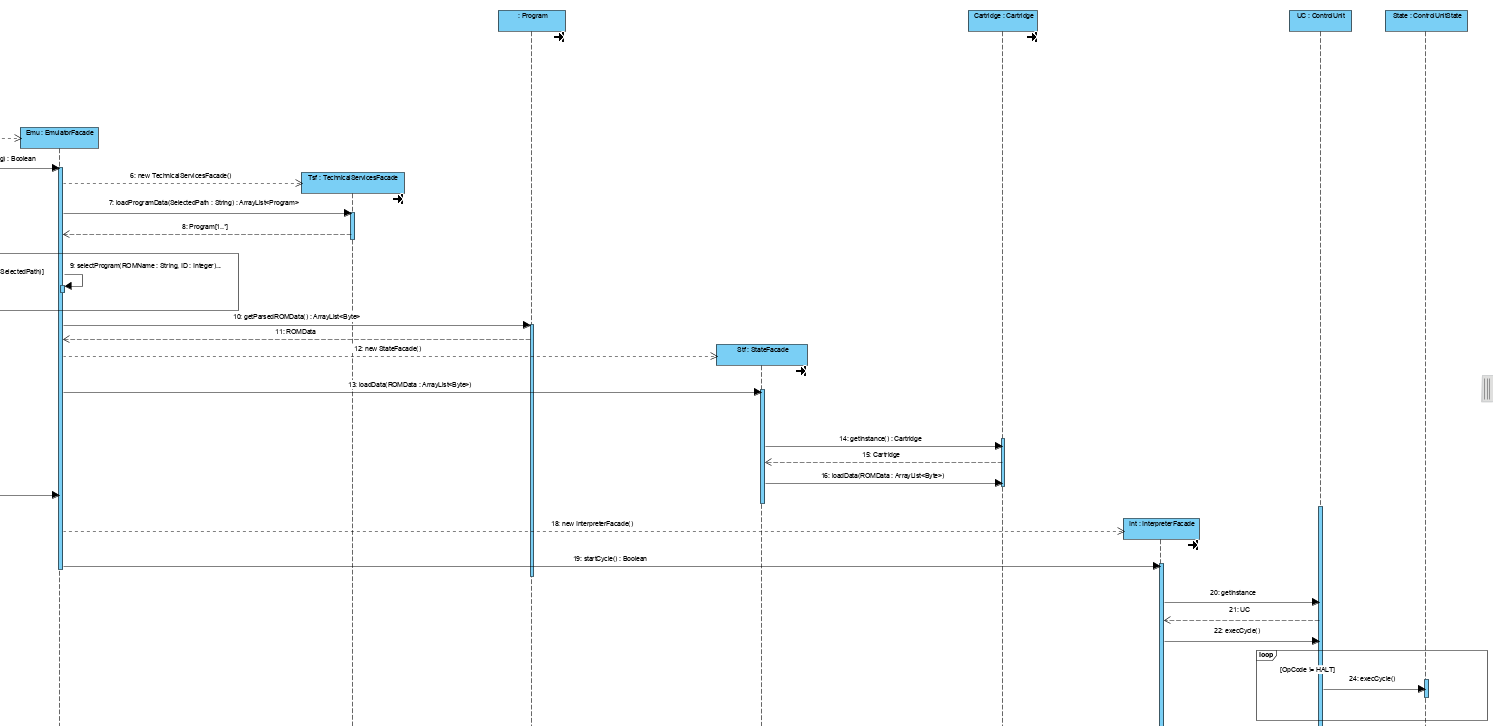
\includegraphics[width=600px, height=281px]{SQD_EseguiProgramma_2.png}\\
	\end{subfigure}
	\small\textbf{SQD\_EseguiProgramma}
\end{figure}\\
In questo diagramma anticipiamo subito che abbiamo, per ora, trascurato la parte che riguarda il recupero dello stato dal programma in esecuzione, per concentrarci sugli input che l'utente fornisce per l'esecuzione del programma. Oltretutto è ben chiaro che, a partire dall'\emph{EmulatorFacade}, avviene il caricamento dei programmi dalla fonte di dati persistente; a tal proposito, è opportuno fare una parentesi. All'utente, il meccanismo di scelta di un file dal File System, oppure dal Database, è totalmente trasparente: l'unica cosa che cambia per l'utente è la selezione di un elemento navigando nel File System dall'interfaccia (che si tradurrà semplicemente nel parsing del file selezionato con il path che porta a quel file), oppure la selezione di un elemento da una \emph{lista}, dove in quest'ultimo caso la selezione avverrà dal File System. La gestione è molto semplice: la selezione di un elemento dalla lista non necessita di un path, bensì solamente di ID e nome; la sola presenza di un ID e un nome, e una stringa vuota passata come parametro in \emph{initProgram()} a \emph{EmulatorFacade}, consentirà di discriminare quella inizializzazione come indirizzata verso il Database, e viceversa avviene per la selezione di un file dal File System.\\
Chiusa questa breve parentesi, si nota come l'intera logica è spostata dalla fonte di dati persistente, all'interno dell'applicazione: si è scelto, quindi, di non effettuare una ricerca del particolare programma nel Database, ma di limitarsi a selezionare tutti i programmi, ed effettuare una piccola ricerca una volta che l'EmulatorFacade è stato fornito di tutti i programmi memorizzati sul Database.\\
Quando si è ottenuto il programma giusto, si passa al caricamento, mediante lo \emph{StateFacade}, dei dati; attenzione: i dati, che sono memorizzati come una stringa all'interno di un oggetto istanza della classe \emph{Program}, devono essere \emph{tradotti} in dati binari per il corretto \emph{innesto} della cartuccia. Una volta tradotti i dati, la classe \emph{Cartridge} effettuerà tutte le operazioni per collocare correttamente i dati nelle memorie giuste da essa mantenuta.\\
Successivamente, infine, tutto è pronto per eseguire il programma, e difatti questa cosa avviene tramite una chiamata \emph{startCycle()} inoltrata verso l'\emph{InterpreterFacade}, che poi chiama \emph{execCycle()} verso la \emph{ControlUnit}, che porta dapprima, così come previsto nel diagramma degli stati, a eseguire la routine contenuta nello stato di \emph{reset} per inizializzare la struttura, e successivamente partire col ciclo di Von Neumann.

Presentiamo in questa istanza anche la comunicazione che avviene tra la CPU e gli altri componenti. È importante comprendere che ogni dispositivo con cui vuol comunicare la CPU è individuato da un certo range di indirizzi. Per fare un breve esempio, se la classe \emph{OperativeUnit} richiama la funzione \emph{read()} sulla classe \emph{Bus}, in base al valore (convertito in esadecimale) del valore passato in ingresso a tale funzione, solo uno tra i dispositivi interessati verrà interpellato: per il range di indirizzi che va da 0x0000 a 0x1FFF è la memoria RAM che verrà interpellata, e così similmente la logica vale per tutti gli altri dispositivi attaccati al \emph{Bus} della CPU.
\clearpage
Mostriamo quindi, per terminare la vista della dinamica che interessa tutte le entità, il diagramma associato, per la corrente iterazione, alla lettura da parte della CPU inoltrata verso il Bus:
\begin{figure}[h]
\centering
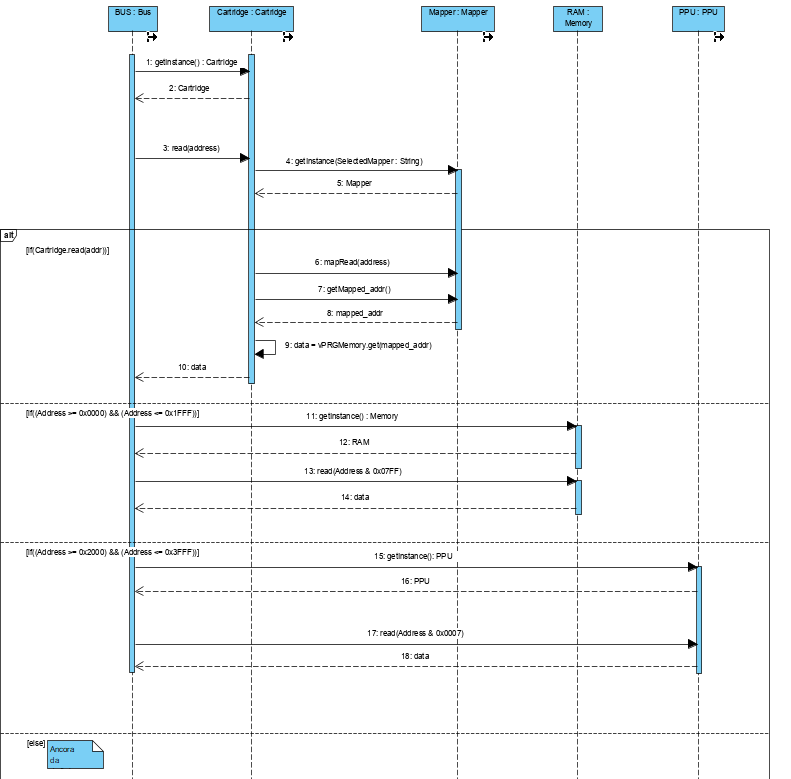
\includegraphics[width=400px, height=400px]{SQD_read().png}\\
\small\textbf{SQD\_read()}
\end{figure}


\clearpage
\subsubsection{Vista componenti\&connettori}
In questa iterazione c'è una piccola modifica alla vista C\&C; nella prima iterazione abbiamo posto poca importanza al recupero di dati dalle fonti persistenti, ipotizzando ci fosse solamente il File System a intervenire come sorgente. In realtà, come abbiamo ampiamente discusso, è presente un Database locale al componente \emph{Emulator}. Pertanto, sussistono delle piccole modifiche al catalogo dei componenti e al diagramma componenti\&connettori:
\begin{figure}[!h]
\hspace*{-1.7cm}
\centering
	\begin{subfigure}{200px}
	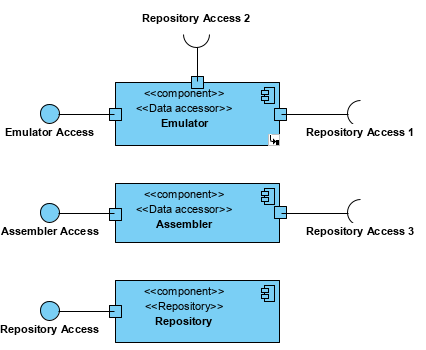
\includegraphics[width=200px, height=166px]{CMPD_NES_Catalogue_1.png}
	\end{subfigure}
	\begin{subfigure}{200px}
	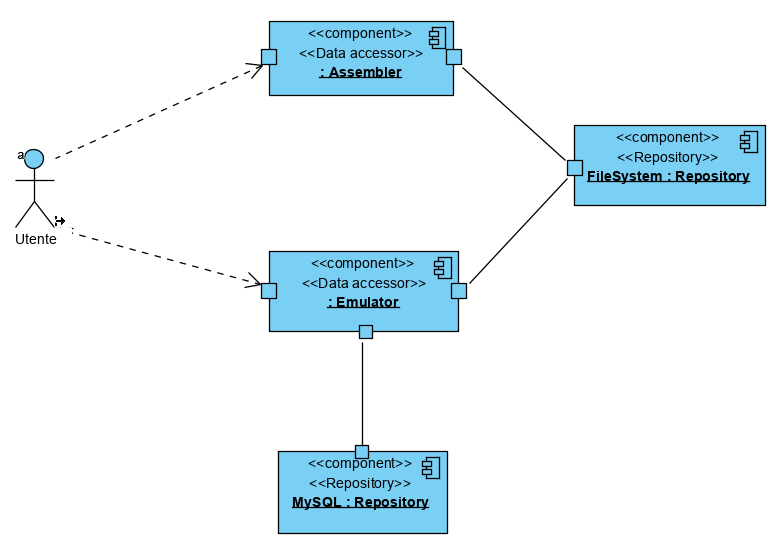
\includegraphics[width=200px, height=144px]{CMPD_NES_1.png}
	\end{subfigure}\\
	\small\textbf{Catalogo dei componenti e annesso diagramma}
\end{figure}

\clearpage
\subsection{Terza iterazione}
In questa terza iterazione le scelte di design sono state per lo più rivolte all'evoluzione della logica applicativa, in quanto una parte \emph{fondamentale} dell'emulatore dovrà essere qui sviluppata, ossia la parte inerente al \emph{rendering grafico}, oltre che ovviamente alla gestione opportuna delle richieste di I/O, e all'aggiunta della gestione delle interruzioni.
\subsubsection{Architettura logica dell'emulatore}
\paragraph{Gestione delle interruzioni, del ciclo della PPU e della tempificazione} Introdurre la gestione delle interruzioni è stato particolarmente semplice, proprio grazie alle scelte di design fatte nelle precedenti iterazioni. È infatti bastato aggiungere un controllo al termine dello stato di \emph{execute} per verificare se ci fosse una richiesta di interruzione (la richiesta di interruzione è mantenuta da degli attributi interni alla classe \emph{OperativeUnit}). Una piccola parentesi va però aperta: il controllo delle interruzioni non è fatto solamente in sincronia col ciclo usuale della CPU; poichè interviene all'esecuzione anche la PPU, un dispositivo indipendente, nella sua esecuzione, dalla CPU, il controllo della presenza di una richiesta di interruzione va fatta anche nel caso in cui la CPU stia attenendo di eseguire, ossia nello stato di fetch. Fatta questa puntualizzazione, possiamo mostrare il diagramma degli stati ulteriormente arricchito nella successiva pagina.
\begin{figure}[h]
\hspace*{-1.7cm}
\centering
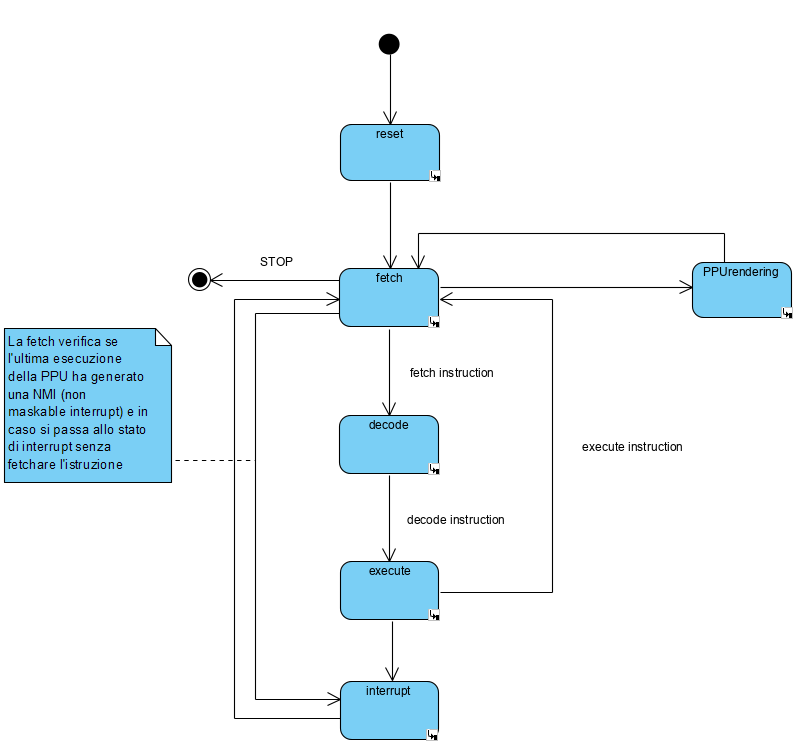
\includegraphics[width=450px, height=415px]{SD_ControlUnit_2.png}\\
\small\textbf{SD\_ControlUnit}
\end{figure}
\clearpage
Come si vede, a partire dalla fetch è possibile passare direttamente allo stato PPUrendering, che è ulteriormente specificato in altri tre stati. Il motivo di ciò sta nel fatto che la PPU è a sua volta una macchina complessa, la cui descrizione necessita di combinare più viste. Consideriamo dunque gli stati interni a questo macrostato nel successivo diagramma degli stati \texttt{SD\_PPU\_rendering}
\begin{figure}[h]
\centering
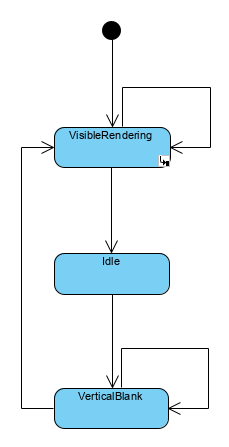
\includegraphics[width=150px, height=295px]{SD_PPU_rendering.png}\\
\small\textbf{SD\_PPU\_rendering}
\end{figure}\\
In questo diagramma tra i tre stati, sicuramente quello più complicato è il \emph{VisibleRendering}. In questo stato vengono, difatti, sviluppate tutte le operazioni, accuratamente tempificate, per renderizzare a video le informazioni contenute nella VRAM.
\clearpage
\paragraph{Gestione dell'I/O}
La gestione dell'I/O ha seguito direttamente quanto è stato nuovamente aggiunto nel \emph{Domain Model} precedentemente presentato in analisi. Sono state fatte modifiche sostanziali al package \emph{State}, e sono state fatte in maniera tale da consentire la corretta ripartizione del lavoro tra i membridel gruppo, e dominare quanto più la complessità. Infatti la suddivisione in package ha aiutato a dare una comprensione astratta di quali erano gli elementi che bisognava isolare e modellare. 
\begin{figure}[!h]
\vspace*{-4cm}

\centering
	\begin{subfigure}{600px}
	\hspace*{-4.3cm}
	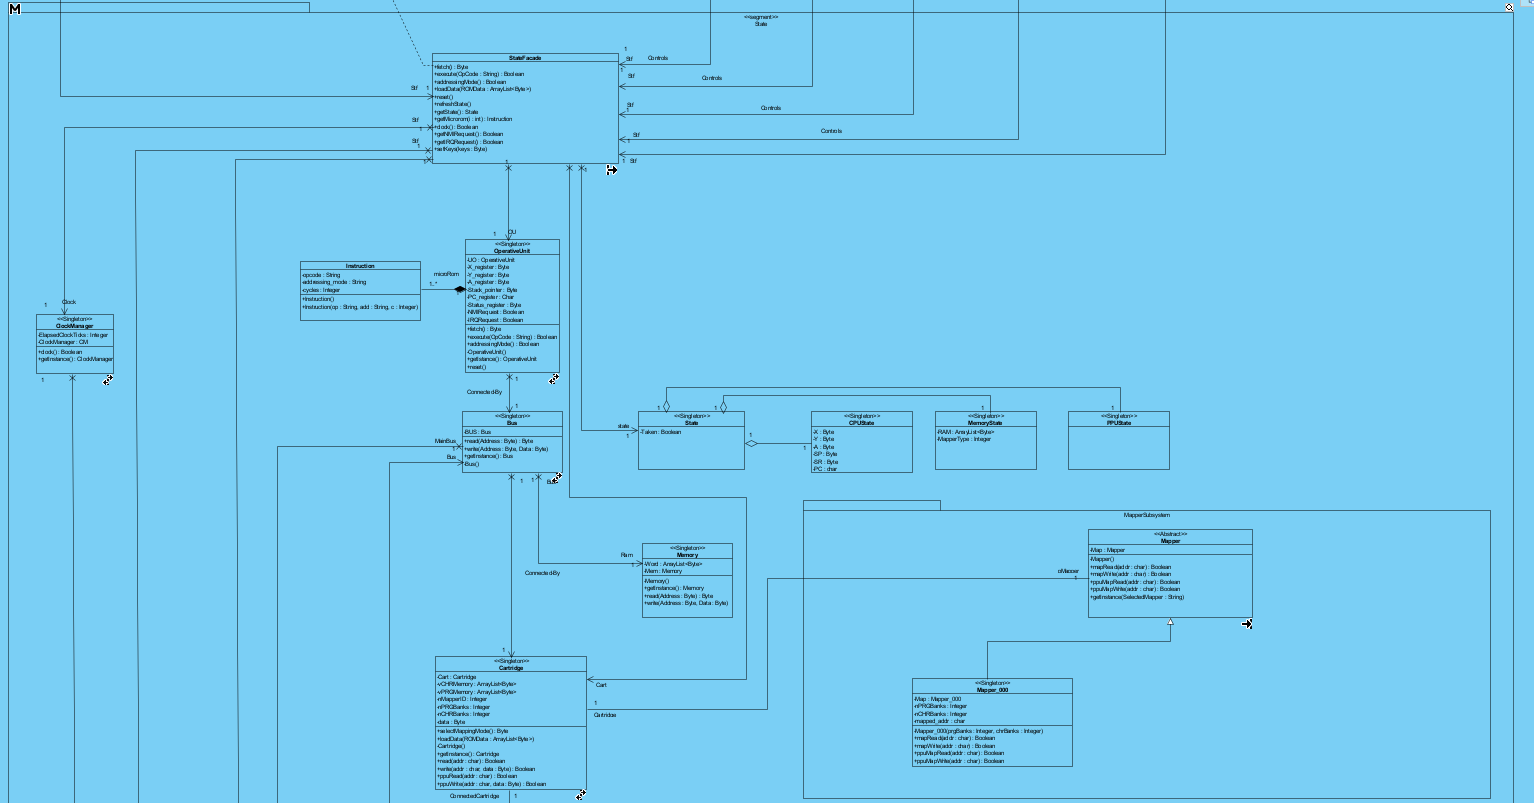
\includegraphics[width=600px, height=314px]{CD_Emulator_4.png}\\
	\end{subfigure}
	\begin{subfigure}{600px}
	\hspace*{-4.3cm}
	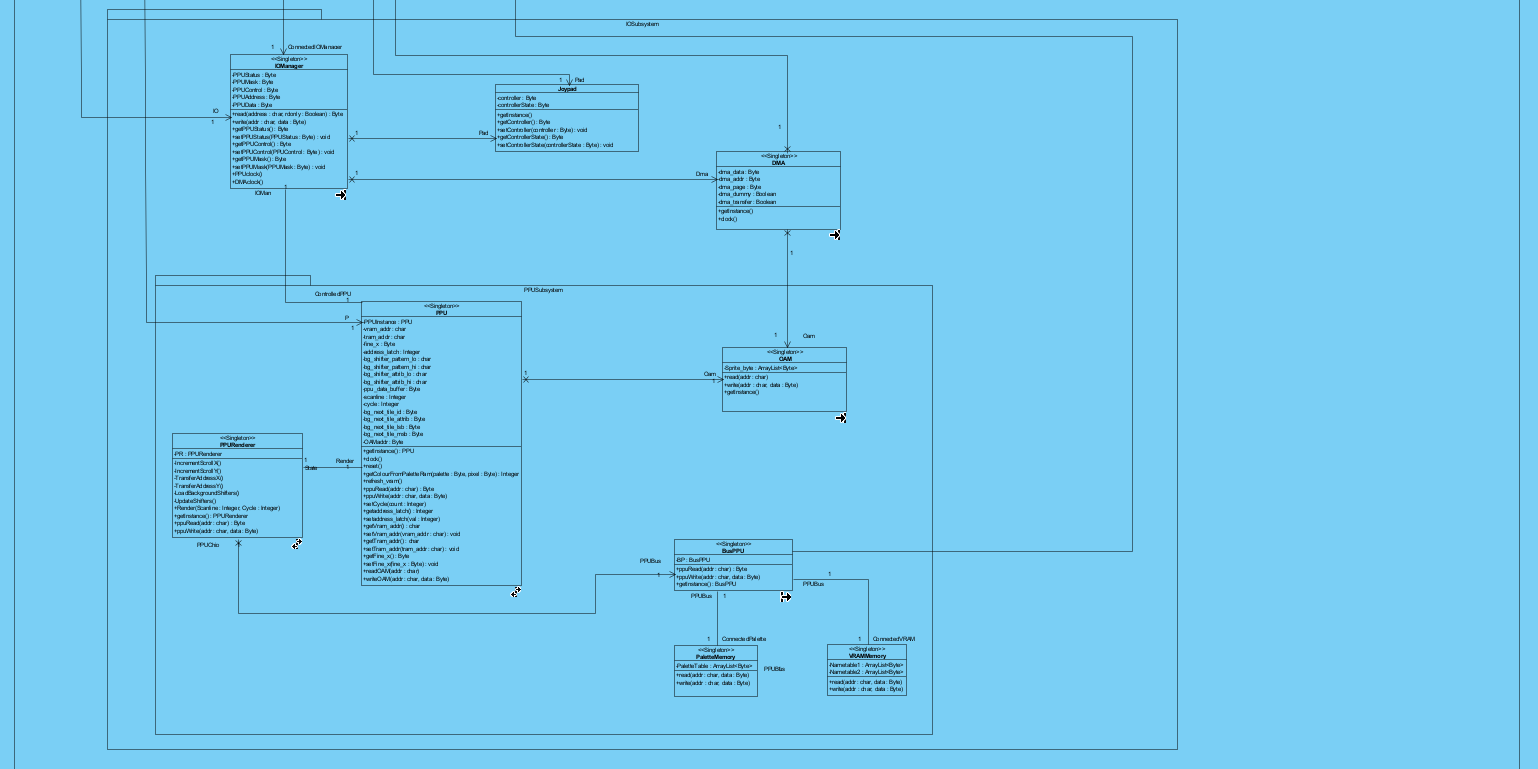
\includegraphics[width=600px, height=300px]{CD_Emulator_5.png}\\
	\end{subfigure}
	\small\textbf{CD\_Emulator}
\end{figure}\\
Procedendo con ordine, possiamo sin da subito notare l'aggiunta di \emph{ClockManager}, a cui è demandata la gestione della tempificazione. Poichè il \emph{ClockManager} si occupa di innescare il clock verso la CPU o le altre periferiche, dato che le periferiche sono molte, abbiamo deciso di redirezionare la decisione di innesco del clock in specifiche funzioni messe a disposizione dalla classe \emph{IOManager}.\\
Come possiamo vedere, è stato aggiunto un altro, grande package, che si chiama \emph{IOSubsystem}. Le responsabilità attribuite agli elementi contenuti nel package sono chiare, e riguardano, ad esempio, la comunicazione con il Bus da parte del DMA per il trasferimento dei dati diretto Cartridge - PPU, la ricezione dei controlli dall'esterno da parte del Joypad, e così via. Ovviamente, tutto quanto è coordinato dall'IOManager, che cerca di catturare tutte le richieste che sono inoltrate verso questo package. Da notare che anche la PPU è trattata dalla CPU come una periferica esterna; nella fattispecie, i registri memory-mapped per la comunicazione con la PPU sono mantenuti, per praticità, nell'IOManager: la comunicazione della CPU verso la PPU, o viceversa, è consentita tramite l'ausilio di questi registri.
\clearpage
Ovviamente la presenza di questo livello di indirezione necessita un'opportuna modellazione, a meno di non incorrere in incomprensioni o imprecisioni. L'impatto verso il Bus è minimale: se quest'ultima classe riceve una richiesta di lettura verso un indirizzo che fuoriesce dal range che va da 0x0000 a 0x3FFF, tutte le richieste vengono inoltrate all'IOManager, che si occuperà lei, invece, di redirezionare in maniera corretta le richieste. Questa cosa è agevolmente specificabile attraverso dei sequence diagram; mostriamo quello relativo alla lettura, omettendo di specificare tutti i dettagli, ma mettendo enfasi soprattutto sulla questione che riguarda lo smistamento delle richieste verso le opportune periferiche.

\begin{figure}[!h]
\vspace*{-4cm}

\centering
	\begin{subfigure}{600px}
	\hspace*{-4.3cm}
	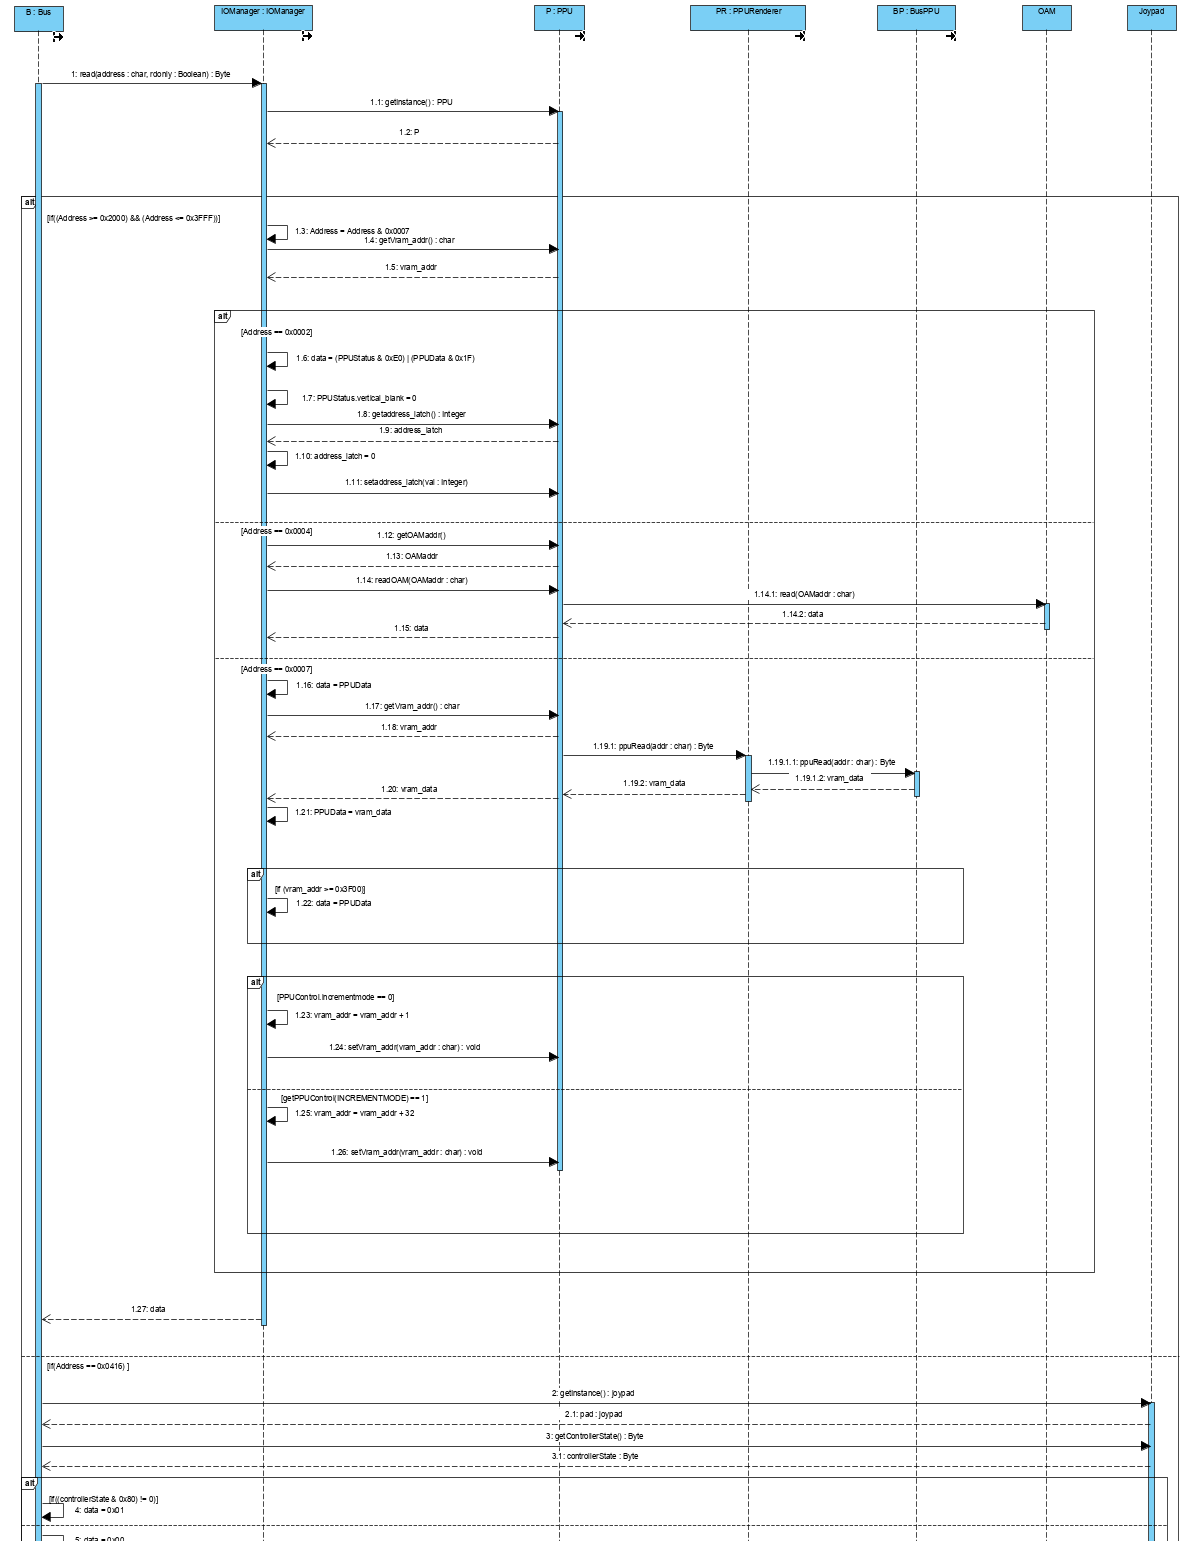
\includegraphics[width=600px, height=789px]{SQD_IORead.png}\\
	\end{subfigure}
\end{figure}
\clearpage

\paragraph{Trasporto dello stato}
Fino a questa iterazione trasportare lo stato non è stato obbiettivo primario del progetto; data la sua importanza, è conveniente che venga qui esplicitata la gestione di questo trasferimento. Bisogna ammettere, tuttavia, che nel trasporto dello stato insiste un problema: la relativa lentezza con cui le informazioni vengono trasportate dall'applicazione verso l'interfaccia grafica. In effetti, la necessità di dover dapprima incapsulare lo stato in un oggetto apposito, trasportare tale oggetto verso il controller, che successivamente comunicherà lo stato trasformato, porta a non avere le migliori performances per l'esecuzione di videogiochi.\\
In ogni caso, il trasporto possiamo descriverlo introducendo quel che è il contenuto del layer `Controller':
\begin{figure}[h]
\hspace*{-2cm}
\centering
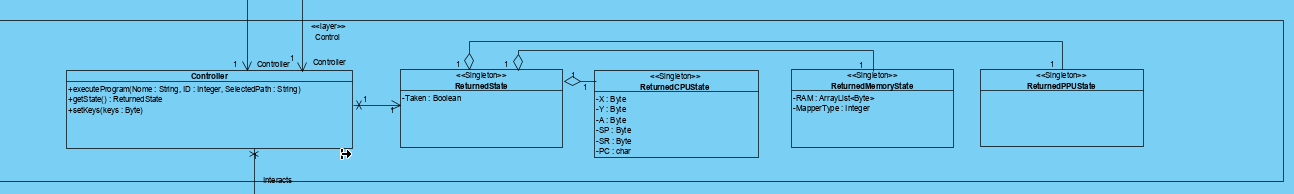
\includegraphics[width=500px, height=74px]{CD_Emulator_6.png}\\
\small\textbf{CD\_Emulator}
\end{figure}\\
In questo layer è presente in special modo una classe, definita \emph{ReturnedState}, che viene popolata alla chiamata verso il Controller di \emph{getState()}. Questa chiamata determina l'aggiornamento dello stato e il conseguente ritorno di tale stato verso la GUI, che potrà quindi aggiornare i parametri mostrati.\\
È necessario che esista un thread costantemente in polling verso il controller, che richieda continuamente lo stato. Per non incorrere in eccessiva lentezza, abbiamo scelto che le richieste non vengano sincronizzate con la pubblicazione di un nuovo stato, e quindi l'accesso a `ReturnedState' non è disciplinato da costrutti come semafori di mutua esclusione o pattern di comunicazione tra threads come produttore/consumatore.

Questo trasporto dello stato è in parte palesato dal raffinamento del diagramma di sequenza associato a \emph{EseguiProgramma}; in questo diagramma è stato aggiunto il punto in cui vengono creati i thread per l'esecuzione del motore del sistema software e per l'accolta degli input esterni dell'utente (per, ad esempio, direzionare i comandi del controller verso la classe Joypad presente nel class diagram).

\paragraph{Gestione della PPU}
La gestione della PPU è la parte cruciale di questa iterazione, in quanto, come già ribadito, sarà il motore che consentirà di effettuare il rendering grafico della ROM che sta venendo eseguita. Assodata la corretta tempificazione, diciamo sin da subito che è vero che lo stato viene ritornato all'interfaccia grafica mediante un'esplicita chiamata verso il controllore da parte di un thread per il recupero dello stato, ma è pur vero che lo stato della PPU, che alla fine consta dei nuovi pixel che sono stati renderizzati, è aggiornato dalla PPU stessa, la quale va a richiamare l'aggiornamento verso la classe \emph{PPUState} presente nel package \emph{State}.

Detto ciò, la gestione della PPU parte dall'esplicazione di quello che è lo state diagram che abbiamo precedentemente presentato nel contesto del macrostato \emph{VisibleRendering}. Per questo macrostato è stato associato un sequence diagram che ben riassume tutto ciò che svolge la PPU nel renderizzare i pixel da far mostrare successivamente a schermo.\\
Innanzitutto mettiamo enfasi sul fatto che il meccanismo della PPU è stato distribuito in due classi, che sono:
\begin{itemize}
	\item{
		PPU.
	}
	\item{
		PPURenderer.
	}
\end{itemize}
In \emph{PPU} sono state incapsulate tutte le informazioni inerenti allo stato interno di tale dispositivo, tra cui ricorrono alcuni registri interni (come \emph{vram\_addr} e \emph{tram\_addr}), e gli shift-registers necessari per memorizzare i tile presenti e successivi da renderizzare. Non solo: la PPU mantiene anche le informazioni relative ai cicli che sono trascorsi, e alla corrente scanline da renderizzare.\\
In \emph{PPURenderer} sono scandite tutte le responsabilità che riguardano in prima persona il rendering dei pixel. Questa cosa non è banale: per renderizzare i pixel è opportuno suddividere ogni singola operazione in metodi a parte per ridurre la complessità totale del rendering e concentrare le responsabilità in parti ben distinguibili dell'architettura. È stato anche deciso, data la frequenza dell'accesso verso le memorie della PPU, di inserire il riferimento al \emph{PPUBus} all'interno del Renderer, per fare in modo che l'accesso verso la memoria fosse più agevolato in fase di rendering.\\
Per comprendere a pieno come sono state pensate e modellate tutte le operazioni inerenti al rendering grafico, bisogna necessariamente consultare tutti i sequence diagram; tuttavia presenteremo qui solamente quello che richiama il render grafico, in quanto è quello principale, che alla fine del rendering del singolo pixel, consentirà l'estrazione del colore corretto e lo predisporrà per la mostra a video da parte dell'interfaccia grafica. Un'altra puntualizzazione è che lo stato della PPU è aggiornato ogniqualvolta tre pixel vengono renderizzati; dunque il flusso prevede che ogni tre colpi di clock, \emph{PPUState} venga aggiornato, e a quel punto tre nuovi pixel possono essere disegnati sullo schermo.\\
Non rimane, quindi, che presentare la funzione che rappresenta il flusso principale che parte dalla PPU e termina con la determinazione finale del pixel, ossia \emph{clock()}. Tale funzione è stata modellata tramite l'ausilio di un sequence diagram, che viene presentato nella successiva pagina.
\begin{figure}[!h]
\vspace*{-4cm}

\centering
	\begin{subfigure}{600px}
	\hspace*{-4.3cm}
	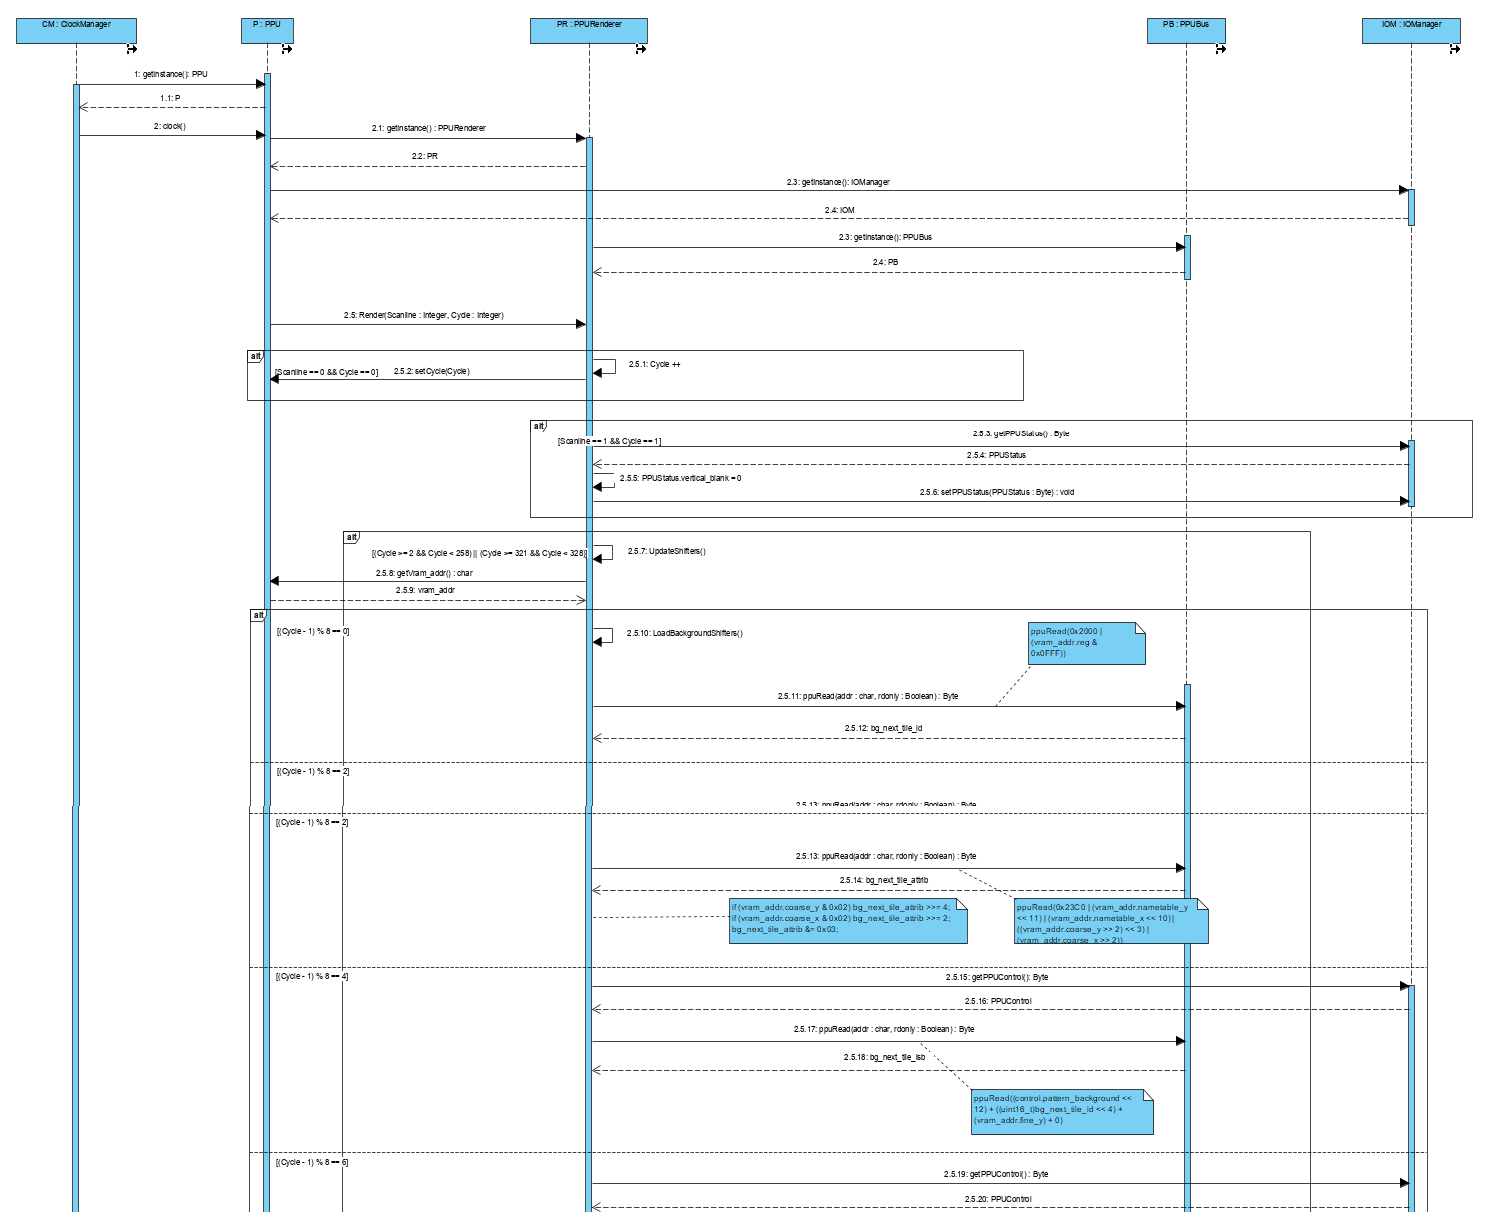
\includegraphics[width=600px, height=789px]{SQD_VisibleRendering.png}
	\end{subfigure}
\end{figure}
\begin{figure}[!h]
\hspace*{-4.3cm}
\centering
\includegraphics[width=600px, height=325px]{SQD_VisibleRendering_2}\\
	\small\textbf{SQD\_VisibleRendering}
\end{figure}\\
Analizzare tutto il diagramma non è semplice, tuttavia ha particolare importanza una delle ultime funzioni che la PPU richiama su sè stessa, ossia \emph{extractPixel()}. Quando questa funzione viene richiamata, vuol dire che si è pronti, secondo il meccanismo ispezionato in analisi, a ricavare il colore del pixel e la sua posizione nello schermo mediante la combinazione delle informazioni tratte dagli shift-registers interni alla PPU che la classe \emph{PPURenderer} ha manipolato nel corso delle chiamate inoltrate ad essa.

In ultimo, ma ovviamente non è trascurabile, abbiamo l'incremento dei cicli trascorsi e della `scanline' da manipolare alla prossima chiamata, ovviamente secondo tutte le particolarità del caso.

\clearpage

\subsubsection{Interfaccia Grafica}

Arrivati alla terza iterazione abbiamo cominciato a porci il problema circa il prelievo dei dati dall'application logic.\\
Abbiamo previsto infatti che tutte le informazioni relativamente al modello sottostante vengano incapsulate in una apposita classe \textbf{ReturnedState}, che viene inoltrata dal controller vers la vista, previa una opportuna richiesta da parte dell'Emulator Boundary.\\

Giunti a questo punto infatti, prevediamo dei poter implementare anche la prima parte della PPU, relativa al rendering del backgroun, e di conseguenza dobbiamo sia poter mostrare a schermo il contenuto di registri e memoria, che naturalmente il primo rendering grafico.\\

Tale sfida è risultata piuttosto insidiosa in quanto la comunicazione, prevista mediante thread, verso il basso, potrebbe incorrere in problemi di concorrenza, e ciò naturalmente ci pone davanti alla scelta di un meccanismo di sincronizzazione.\\
Da un lato si sarebbe potuto realizzare uno stile ad eventi del tipo publish/subscribe, mediante un mediatore opportuno. Tuttavia tale scelta è stata scarta a causa della eccessiva lentezza di tale approccio : prevedere infatti un meccanismo di sospensione e notifica avrebbe rallentato eccessivamente il sistema, rendendo il rendering a video troppo lento e non soddisfacente.\\

Abbiamo infatti stabilito, di non utilizzare particolari tipi di controllo, se non l'accesso sincronizzato ai metodi delle classi singleton, per evitare inconsistenza nella creazione degli stessi.\\
Così facendo abbiamo anche pensato al meccanismo di prelievo, per il quale l'emulator boundary, tramite un thread appositor richiede lo stato verso il controllore, il quale si occupa di fornirlo internamente alla classe returned state citata in precedenza.\\

Una volta ottenuto tale stato, l'EmulatorBoundary provvede ad aggiornare le classi del package DisplayBoundary; \\
Ciò ci ha portati naturalmente ad arricchire le classi di tale package, aggiungendo una nuova entità delegata alle operazioni "artistiche" e al rendering grafico dello schermo, denominata \textbf{Screen}.\\
Tale classe farà largamente uso del framework da noi scelto per poter renderizzare a schermo pixel per pixel il contenuto inoltrato dalla PPU verso l'alto,e sarà opportunamente aggiornata per mano del DisplayBoundary, sotto richiesta dell'Emulator Boundary.\\

Successivamente il DisplayBoundary potrà aggiornare lo stato visibile della CPU, della memoria e della PPU, come possiamo apprezzare dal seguente diagramma di sequenza:

\begin{figure}[!h]
\vspace*{-4cm}

\centering
	\begin{subfigure}{600px}
	\hspace*{-3cm}
	\includegraphics[width=550px, height=180px]{SQD_UpdateDisplayBoundary.png}\\
	\end{subfigure}
\end{figure}
\clearpage



\clearpage
\subsection{Quarta iterazione}
\subsubsection{Gestione della lista dei programmi}
La gestione della lista dei programmi avviene esponendo verso il layer \emph{GUI} alcuni metodi contenuti all'interno del controllore. In effetti, il package \emph{Controller} subisce, in questa iterazione, una lieve modifica, che qui di seguito mostriamo:
\begin{figure}[h]
\hspace*{-2.7cm}
\centering
\includegraphics[width=500px, height=61px]{CD_Emulator_7.png}\\
\small\textbf{CD\_Emulator}
\end{figure}\\
In particolar modo interessa la classe a sinistra, nominata \emph{ReturnedProgram}; il Controller farà in modo di ritornare oggetti di questo tipo verso l'interfaccia quando richiesto, ad esempio attraverso il metodo \emph{getProgramList()}. Non solo: il Controller espone metodi come \emph{insertProgram()} e \emph{deleteProgram()} che sono utili alla gestione della lista.\\
La gestione di come queste operazioni vengano redirezionate verso le giuste fonti persistenti viene attuata dalle classi presenti nel package \emph{TechnicalServices}, sulla base dei parametri che vengono passati al Controller.
\begin{figure}[h]
\hspace*{-4.2cm}
\centering
\includegraphics[width=600px, height=368px]{CD_Emulator_8.png}\\
\small\textbf{CD\_Emulator}
\end{figure}\\
Nella successiva pagina viene mostrato il package TechnicalServices, che varia proprio per i metodi contenuti nelle varie classi. Nel caso di \emph{insertProgram()} è stato anche previsto un inserimento da Database verso il File System (in base a se sono stati passati una stringa vuota e un numero pari a -1 per il nome e l'ID del programma), ma nella fattispecie l'interfaccia non ne fa mai uso. Per tale motivo, mostriamo solamente, tramite un sequence diagram, come viene gestito l'inserimento di un programma da File System verso il Database.\\
Come si può facilmente notare, è stata riciclata la funzione che consentiva il recupero di un file da FileSystem: la cosa è conveniente, basta specificare da quale file si sta leggendo, e successivamente fare le opportune chiamate, col programma recuperato, per scrivere tale programma sul DataBase, avendo l'accortenza ovviamente di recuperare il giusto nome da inserire nella tabella.
\begin{figure}[h]
\hspace*{-4.2cm}
\centering
\includegraphics[width=600px, height=258px]{SQD_InsertProgram.png}\\
\small\textbf{SQD\_InsertProgram}
\end{figure}
\clearpage
\subsubsection{Gestione del trasporto dello stato e dei flussi d'esecuzione concorrenti}

Arrivati alla quarta iterazione è diventato imperativo poter suddividere correttamente la logica di esecuzione, in realzione ai flussi concorrenti, così come era stato postulato all'inizio del progetto. ciò è fondamentale per la gestione degli input utente, sia per poter controllare l'esecuzione del programma, ma anche per poter inoltrare gli input del \emph{joypad} verso il basso.\\
è inoltre necessario scindere correttamente il flusso esecutivo tramite tre thread ben precisi:

\begin{enumerate}
\item{
\textbf{LogicThread} : Thread relativo all'avvio del motore logico
}
\item{
\textbf{PollingThread} : Thread relativo al prelievo dei dati, in polling, dello stato sottostante,e quindi responsabile anche all'aggiornamento del DisplayBoundary,
}
\item{
\textbf{UserInputThread} : Thread in ascolto degli input utente. Tali input saranno redirezionati verso il motore in caso di pressione di tasti utili al joypad, altrimenti saranno utilizzati per controllare il flusso di esecuzione del LogicThread
}
\end{enumerate}

Abbiamo quindi effettuato un cambiamento di rotta, in quanto adesso i flussi concorrenti saranno in totale 3, e la stessa interfaccia relativa al DisplayBoundary incapsulerà i frame relativi alle periferiche da mostrare; ciò ci ha garantito una semplicitià nello sviluppo maggiore, oltre che una resa grafica più compatta e \emph{user friendly}.

Per quanto ne concerne i tre flussi principali, come già detto, essi saranno creati dall'EmulatorBoundary a seguito della selezione e dell'avvio del programma;\\
per descrivere opportunamente tali thread abbiamo fatto ricorso a dei diagrammi degli stati, già ampiamente utilizzati durante tutto il progetto, che si sono dimostrati una risorsa quanto mai utile per modellare il comportamento di tutto il nostro software.\\

Per sinteticità mostreremo solo la modellazione del thread \emph{Polling}, in quanto la modellazione degli altri thread sarà decisamente simile a quanto proporremo, poichè ci baseremo su una strutturazione piuttosto comune ad ogni thread, lasciando il dettaglio del funzionamento concreto dello specifico thread ai Sequence Diagram relativi, fornendo quindi una \emph{prospettiva} diversa sui funzionamenti proposti fino ad ora.\\

\begin{figure}[h]
\hspace*{-1.7cm}
\centering
\includegraphics[width=250px, height=215px]{SD_Polling.png}\\
\small\textbf{SD per il thread Polling}
\end{figure}

Ogni flusso esecutivo dovrà dapprima essere creato, per poi essere messo in esecuzione. Lo stato così descritto, ovvero un \textbf{macrostato}, è quello di Runnable, che incapsula l'esecuzione specifica del processo.\\ 
Naturalmente il flusso esecutivo potrà passare nello stato Suspended se sospeso da parte del flusso di gestione degli input, oppure terminare una volta svolto il suo compito, che si traduce nella terminazione del programma stesso.\\

\begin{figure}[h]
\hspace*{-1.7cm}
\centering
\includegraphics[width=250px, height=215px]{SD_CheckForUpdates.png}\\
\small\textbf{SD per il macro stato del thread di Polling}
\end{figure}

Nel macrostato Runnable, dobbiamo distinguere lo stato di Ready, in cui il task si trova qualora lo scheduler del sistema operativo lo prealzioni. Altrimenti il fusso procede effettuando un \emph{checkforupdates} e successivamente passando in uno stato di \emph{Update Display}; entrambi gli stati possono essere efficacemente descritti mediante 
il sequence diagram già presentato a riguardo.

\subsubsection{Interfaccia grafica}

Giunti nella fase finale dello sviluppo, almeno per quanto ne concerne la consegna del progetto, abbiamo raffinato quanto già modellato in termini di vista statica.\\
il diagramma delle classi infatti faceva riferimento a 3 classi relative ai frame per PPU,CPU e Memoria, che sono stati in realtà eliminati durante il refinement di questa fase.\\

abbiamo infatti convenuto che la presenza di così tante classi non fosse necessario, specialmente in quanto il numero di entità da mostrare nel display boundary era diventato
vertiginosamente più alto. Allo stato attuale invece l'interfaccia presenta una serie di pannelli, selezionabili dinamicamente, che mostrano opportunamente il contenuto dello stato
estratto dal motore sottostante.\\ 

L'interfaccia DisplayBoundary prevede ora una serie di metodi che le vengono richiamati dal Polling Thread, in continuo aggiornamento; tali metodi
permettono l'update non solo dello screen, ma anche della visualizzazione di RAM, VRAM, Palette Rame, OAM, nonchè della PPU e della CPU.\\

Il package DispalyBoundary diventa così sufficientemente compatto, ed in grado di realizzare buona parte delle funzionalità che ci eravamo preposti all'inizio dello sviluppo.\\
Manca ancora tuttavia una esplicita gestione alla cattura degli input utente per la sospensione del programma in esecuzione, ma abbiamo ritenuto più che soddisfacente il livello raggiunto per questa attuale iterazione.\\

A voler essere onesti, dobbiamo segnalare un problema sostanziale con quanto fatto fino ad ora : un sistema a livelli, con un prelievo dati dal modello, e non dai technical services, non è particolarmente performante o adatto per un rendering così tanto dinamico come quello che stiamo presentando.\\
Infatti per una interazione con l'interfaccia così attiva, si sarebbe prestato meglio un modello MVC, con uno stile ad invocazione implicita, oppure un pattern Observer; scelte asincrone infatti ci avrebbero permesso di ottimizzare le prestazioni e rendere l'aggiornamento dei dati meno convoluto e farraginoso di quanto invece non ci sia risultato.\\

Tuttavia i risultati ottenuti sono quantomeno soddisfacenti, e hanno contribuito ad accrescere la nostra esperienza a riguardo.\\

Di seguito mostriamo uno spaccato del class diagram, completo della modellazione della GUI.

\begin{figure}[h]
\hspace*{-2.7cm}
\centering
\includegraphics[width=500px, height=350px]{CD_GUI_4.png}\\
\small\textbf{Class Diagram : GUI quarta iterazione}
\end{figure}

\subsubsection{Rendering del foreground}

Per renderizzare correttamente gli sprites a schermo sono stati implementati degli aggiornamenti alle logiche della gestione dell' I/O presentate durante la terza iterazione. 
\paragraph{Gestione OAM}
La memorizzazione degli sprites nell' OAM sarà implementata grazie all 'utilizzo del DMA. In particolare, Ogni qual volta che la CPU andrà a scrivere nell'indirizzo 0x4014, essa scriverà la pagina in memoria da dover copiare e, attraverso l'IOManager attiverà automaticamente il DMA, che andrà a copiare l'intera pagina di memoria all'interno dell'OAM.
\begin{figure}[h]
\hspace*{-4.2cm}
\centering
\includegraphics[width=600px, height=80px]{Scrittura_DMA.png}\\
\small\textbf{Avvio DMA}
\end{figure}\\
\paragraph{Sprite Rendering}
Per implementare il rendering del foreground andremo ad utilizzare degli shift register chiamati "sprite\_shifter\_pattern\_lo" e"sprite\_shifter\_pattern\_hi" che allo stesso modo del backgorund contengono le informazioni del prossimo Byte da renderizzare a schermo e permettono di renderizzare un bit alla volta shiftando ad ogni ciclo della PPU di 1. Ma prima i fare questo andremo a capire quali sprite selezionare. \\
Ad ogni scancile, nel ciclo 257 andremo a visualizzare se sono presenti uno o più sprites da renderizzare nella prossima riga e li andremo a inserire in un vettore contente gli sprite da renderizzare chiamato "Sprite\_scanline". In più andremo a controllare se uno degli sprites inseriti è lo sprite 0, e in caso settiamo a true una variabile "bSpriteZeroHitPossible" in modo da gestire la collision Detection che abbiamo discusso nella fase di analisi. Infine se gli sprite da disegnare sono più di 8 allora alzeremo anche il bit di overflow relativo. 
\begin{figure}[h]
\hspace*{-4.2cm}
\centering
\includegraphics[width=600px, height=350px]{Verifica_Sprites.png}\\
\small\textbf{Verifico la presenza degli Sprites}
\end{figure}\\
Una volta salvati gli sprite da renderizzare, nel cilclo 340 andremo a definire l'altezza dello sprite andando a leggere un flag del registro PPUControl e l'orientamento. Se Lo sprite deve essere specchiato verticalmente andremo a invertire gli \emph{indirizzi} mentre se dovrà essere specchiato orizzontalmente andremo a specchiare i \emph{dati} da renderizzare. Presi quindi i bit con il giusto orientamento li andremo a scrivere negli shift register prima citati che conterranno quindi i valori corretti pronti per essere renderizzati a video. \\

\begin{figure}[h]
\hspace*{-4.2cm}
\centering
\includegraphics[width=300px, height=400px]{Sprite_Specchiati_Verticalmente.png}\\
\small\textbf{Verifica orientamento verticale e altezza degli Sprites}
\end{figure}
\begin{figure}[h]
\hspace*{-4.2cm}
\centering
\includegraphics[width=300px, height=100px]{Sprite_Specchiati_Orizzontalmente.png}\\
\small\textbf{Verifica orientamento orizzontale degli Sprites}
\end{figure}

Infine andremo ad estrarre dagli shift register i bit del foreground allo stesso modo del background ma questa volta lo sprite ci darà un informazione anche sulla priorità che ci permetterà di capire quale pixel tra background e foreground verrà stampato a video in una determinata posizione. \\
\begin{figure}[h]
\hspace*{-4.2cm}
\centering
\includegraphics[width=300px, height=400px]{Foreground1.png}\\
\end{figure}
\begin{figure}[h]
\hspace*{-4.2cm}
\centering
\includegraphics[width=300px, height=400px]{Foreground2.png}\\
\end{figure}
\begin{figure}[h]
\hspace*{-4.2cm}
\centering
\includegraphics[width=300px, height=400px]{Foreground3.png}\\
\end{figure}
\begin{figure}[h]
\hspace*{-4.2cm}
\centering
\includegraphics[width=300px, height=100px]{Foreground4.png}\\
\small\textbf{Confronto pixel e palette Foreground/Background}
\end{figure}

\clearpage
\section{Prospettiva implementativa}
In questa sezione è d'interesse mettere enfasi sulle scelte tecnologiche adoperate per lo sviluppo del nostro sistema software, e anche mostrare gli artefatti che ci aspettiamo saranno prodotti al termine del progetto.
\subsection{Prima iterazione}
\subsubsection{Vista di deployment}
In questa prima iterazione ci siamo concentrati su come i componenti, che appiono nell'apposito diagramma dei componenti, vengono manifestati a runtime dai nostri artefatti. Prima di ciò, è bene però specificare che già da qui abbiamo deciso alcune delle tecnologie da utilizzare:
\begin{itemize}
	\item{
		Il linguaggio di programmazione Java;
	}
	\item{
		JRE, l'ambiente di esecuzione che consente di eseguire gli eseguibili prodotti dalla compilazione del codice Java (i bytecodes);
	}
	\item{
		Il File System offerto dall'ambiente d'esecuzione ospite di JRE (nel nostro caso, Windows 10).
	}
\end{itemize}
A questo punto, mostriamo il diagramma di deployment che chiarifica e sintetizza tutte queste informazioni in maniera concisa nella successiva pagina.\\
Come si può notare, abbiamo specificato le istanze dei componenti (come l'emulatore e l'assemblatore) da quali artefatti sono manifestati.
\begin{figure}[t]
\hspace*{-3cm}
\centering
\includegraphics[width=550px, height=300px]{DD_NES.png}\\
\small\textbf{DD\_NES}
\end{figure}

\clearpage
\subsection{Seconda iterazione}
In questa iterazione abbiamo sicuramente l'ausilio di alcuni notevoli framework. Di seguito quindi una breve esposizione di come tali framework sono stati adoperati, lo scopo, e le varie classi che fanno uso dei servizi offerti dal framework.
\subsubsection{Hibernate e vista di deployment}
In vista dell'ausilio di una fonte di dati persistente che non fosse il File System, ci siamo adoperati a scegliere un DBMS e un framework che agevolasse l'interfacciamento con i servizi offerti dal DBMS.\\
La scelta del Database è ricaduta su \emph{MySQL}. Adoperare i driver JDBC e impostare la connessione con MySQL poteva essere una possibile scelta, ma abbiamo deciso di automatizzare quanto più il processo di interfacciamento con il Database, ricorrendo a un framework che consentisse di mappare automaticamente le entità desiderate della nostra logica di business con quelle mantenute dal Database; il framework va sotto al nome di Hibernate: molto semplice da installare e configurare, l'alternativa è tanto semplice da aver reso la classe di interfacciamento al Database, ossia \emph{ProgramDAO}, estremamente semplice nella sua implementazione.

Ovviamente, avendo previsto un Database, e quindi un componente in più, è stato necessario modificare lievemente il diagramma di deploy, che mostriamo nella successiva pagina per completezza.
\begin{figure}[h]
\hspace*{-3cm}
\centering
\includegraphics[width=550px, height=300px]{DD_NES_1.png}\\
\small\textbf{DD\_NES}
\end{figure}
\clearpage

\subsubsection{Java swing }

Per poter realizzare l'interfaccia grafica ci siamo rifatti ad un framework molto documentato e piuttosto intuitivo nel suo utilizzo : \emph{Java Swing}.\\
Dato infatti l'approccio allo sviluppo agile e ovviamente al riuso, ci è sembrata la scelta più utile applicare un framework che mettesse a disposizione una serie di costrutti già preparati ed efficienti per la gestione sia della parte strettamente grafica, che della cattura di input mediante mouse e tastiera.\\

Non solo, JavaSwing si presta anche alla realizzazione di thread concorrenti mediante una classe specifica \textbf{SwingWorker} che mette a disposizione una serie di metodi per la gestione di tali thread. Così facendo, nelle prossime iterazioni, avremo gli strumenti necessari per poter realizzare tutti i flussi concorrenti che si siamo presupposti di gestire.\\

Al contempo, sempre tramite opportune funzionalità di libreria, saremo in grado di gestire anche la resa grafica del rendering del display.\\
\subsubsection{Installazione e configurazione delle librerie}
La configurazione necessaria per effettuare il building del sistema prevede l'ausilio di apposite librerie e file di configurazione, che concernono quasi esclusivamente il necessario per poter interfacciarsi con le fonti di dati persistenti.\\
Innanzitutto è necessario inserire nel \emph{build path} del proprio progetto le librerie richieste per la corretta installazione dei moduli di Hibernate, la libreria che consta dei driver necessari per l'interfacciamento al database MySQL, e il file di configurazione XML per la parametrizzazione di Hibernate.\\
Premettiamo che la procedura è testata sull'ambiente di sviluppo Eclipse.

Per l'installazione delle librerie è sufficiente trascinare queste ultime sul progetto nella finestra a lato sinistro di Eclipse. Le librerie sono fornite nel repository ove è presente il progetto, nella cartella 'librerie'. In questa cartella sono presenti altre tre cartelle, nominate 'hibernate', 'mysql', 'configurazione', dove nelle prime due è possibile trovare tutte le librerie da installare nella repository di progetto, mentre nell'ultima è possibile trovare il file di configurazione XML che hibernate si aspetta di trovare nella cartella 'src' del progetto Java (e quindi è consigliabile inserire tale file di configurazione all'interno di tale cartella).\clearpage
Una volta che tutte le librerie e il file di configurazione sono messi al posto giusto, è sufficiente aggiungere i riferimenti alle librerie nel progetto Java; basta andare sulle proprietà del progetto, cliccare su 'Configure build path' e nella nuova finestra che si mostrerà all'utente cliccare su 'Add JARs', che necessiterà quindi la selezione delle librerie esterne da installare. Se le librerie sono state copiate correttamente nel progetto, i moduli verranno mostrari già all'utente e la selezione sarà immediata.
\begin{figure}[h]
\hspace*{-4.2cm}
\centering
\includegraphics[width=600px ,height=350px]{CONFG.png}
\end{figure}\clearpage
Ovviamente per poter usare MySQL bisogna avere sulla propria macchina un server MySQL attivo; tramite l'ausilio di XAMPP o qualsiasi altro software integrato, la configurazione di MySQL è particolarmente semplice. Di default XAMPP, a meno di avere il porto già occupato, consente l'avvio del server MySQL, attraverso un'interfaccia grafica di immediata comprensione, al porto 3306.
\begin{figure}[h]
\centering
\includegraphics[width=350px, height=225px]{XAMPP.png}
\end{figure}\\
A questo punto, disposti del server, Hibernate potrà avviare la connessione. Per non dover personalizzare la configurazione, e usare la configurazione fornita, bisogna creare uno schema nel server MySQL chiamato \emph{emulator} e aggiungere a questo schema una tabella tramite il seguente script:
\begin{lstlisting}
CREATE TABLE program (    
ID int PRIMARY KEY AUTO_INCREMENT,     
Name varchar(255),    
ROMData LONGTEXT);
\end{lstlisting}
Ovviamente è possibile usare qualsiasi software dotato di interfaccia grafica per l'accesso a MySQL per soddisfare questa semplice richiesta. Nel nostro caso, riteniamo che MySQL Workbench sia più che sufficiente.
\clearpage
\section{Testing}
Per quanto ne concerne il test del sistema, questo è stato un punto piuttosto critico. Testare il corretto funzionamento delle feature da noi pensate e implementate, come il rendering a video del contenuto dei registri e della memoria, oppure la selezione di un programma o l'inserimento in lista di un programma, non è stato difficoltoso.

Tutt'altro discorso però ha resentato il testing relativo a componenti interni come la CPU e la PPU, la cui logica implementativa, decisamente complessa, hanno richiesto l'ausilo di mezzi esterni.

Fortunatamente la scelta di sviluppare un emulatore che avesse come base il processore 6502, e i componenti del NES è stata oculata, e non fatta senza uno studio di fattibilità alla base.

La community relativa alla console è molto attiva e mette a disposizione moltissimo materiale non solo relativo all'architettura in se, per chi fosse interessato a studiarla, come nel nostro caso, ma anche una serie di log e test automatizzati per testare il corretto funzionamento del sistema.

Infatti, una volta completata la CPU, da noi considerata il nucleo fondamentale dell'applicativo, ci siamo concentrati ad effettuare un test quanto più intensivo possibile, mediante un LOG di sistema apposito.

Abbiamo quindi realizzato piccole funzioni di debug per produrre un LOG dell'esecuzione di un programma di test, così da poter confrontare i due log e trovare le discrepanze eventuali, così da andare selettivamente a correggere errori nei codici operativi.

I log di sistema prodotti sono molto lunghi, e non sono particolarmente indicativi per chi non li ha utilizzati, tuttavia mostriamo il log utilizzato  giusto per una manciata di istruzioni:
\begin{lstlisting}
4c c000  A: 0 X: 0 Y: 0 SP: fd SR: 24 JMP ABS CYC: 7
a2 c5f5  A: 0 X: 0 Y: 0 SP: fd SR: 24 LDX IMM CYC: 10
86 c5f7  A: 0 X: 0 Y: 0 SP: fd SR: 26 STX ZP0 CYC: 12
86 c5f9  A: 0 X: 0 Y: 0 SP: fd SR: 26 STX ZP0 CYC: 15
86 c5fb  A: 0 X: 0 Y: 0 SP: fd SR: 26 STX ZP0 CYC: 18
20 c5fd  A: 0 X: 0 Y: 0 SP: fd SR: 26 JSR ABS CYC: 21
ea c72d  A: 0 X: 0 Y: 0 SP: fb SR: 26 NOP IMP CYC: 27
38 c72e  A: 0 X: 0 Y: 0 SP: fb SR: 26 SEC IMP CYC: 29
b0 c72f  A: 0 X: 0 Y: 0 SP: fb SR: 27 BCS REL CYC: 31
ea c735  A: 0 X: 0 Y: 0 SP: fb SR: 27 NOP IMP CYC: 34
18 c736  A: 0 X: 0 Y: 0 SP: fb SR: 27 CLC IMP CYC: 36
b0 c737  A: 0 X: 0 Y: 0 SP: fb SR: 26 BCS REL CYC: 38
4c c739  A: 0 X: 0 Y: 0 SP: fb SR: 26 JMP ABS CYC: 40
ea c740  A: 0 X: 0 Y: 0 SP: fb SR: 26 NOP IMP CYC: 43
\end{lstlisting}

Una volta raggiunto un livello di sviluppo sufficiente a poter effettuare il rendering grafico, ci siamo avvalsi dell'esecuzione della stessa ROM di test : questa permette infatti di effettuare test selettivi, una volta selezionato opportunamente il test dall'emulatore stesso.\\

Ciò ha velocizzato tremendamente il testing, consentendoci di dichiarare funzionante al 100\% la CPU nell'arco di poche ore.

\begin{figure}[h]
\hspace*{+0cm}
\centering
\includegraphics[width=256px, height=240px]{Nestest.png}\\
\small\textbf{ROM di test}
\end{figure}








\end{document}